% Monograph LaTeX Template for UFSC based on:
%
% 1. https://github.com/royertiago/tcc
% 2. http://portal.bu.ufsc.br/normalizacao/
% 3. https://github.com/AdrianoRuseler/abntex2-ufsc

% You need to run `pdfTeX` 5 times on the following order: 1. `pdfTeX`, 2. `biber`, 3. `pdfTeX` 4.
% `pdfTeX` 5. `pdfTeX` 6. `biber` 7. `pdfTeX`, when the bibliography includes a cyclic reference to
% another bibliography, so we need a last pass to fix the bibliography undefined references.

% Includes and fixes several `abntex2` class problems
% Must be included before loading class
%----------------------------------------------------------------------------------------
%   PACKAGES AND OTHER DOCUMENT CONFIGURATIONS BEFORE LOADING abntex2
%----------------------------------------------------------------------------------------

% Uncomment the line `\englishtrue` to set the document default language to english.
%
% Is it possible to keep my translation together with original text?
% https://tex.stackexchange.com/questions/5076/is-it-possible-to-keep-my-translation-together-with-original-text
\newif\ifenglish\englishfalse
\englishtrue

% How to expand \ifthenelse so that it can be used in \parshape?
% https://tex.stackexchange.com/questions/131002/how-to-expand-ifthenelse-so-that-it-can-be-used-in-parshape
\newcommand{\lang}[2]{\ifenglish#1\else#2\fi}

% Disable the empty pages automatically put by memoir class, except the ones by \cleardoublepage
% \PassOptionsToClass{openany}{memoir}

% How to make \PassOptionsToPackage add the option as the last option?
% https://tex.stackexchange.com/questions/385895/how-to-make-passoptionstopackage-add-the-option-as-the-last
\ifenglish
    \newcommand{\swapcontents}[2]{#1 #2}

    \PassOptionsToPackage{language=english}{biblatex}
    \PassOptionsToPackage{brazil,main=english,spanish,french}{babel}
\else
    \newcommand{\swapcontents}[2]{#2 #1}

    \PassOptionsToPackage{language=brazil}{biblatex}
    \PassOptionsToPackage{main=brazil,english,spanish,french}{babel}
\fi




% Applying options to already loaded package
% https://tex.stackexchange.com/questions/124049/applying-options-to-already-loaded-package
%
% For web links and paths with \path{..} and \url{https://www.python.org/downloads/}
% https://tex.stackexchange.com/questions/3033/forcing-linebreaks-in-url
% ftp://tug.ctan.org/pub/tex-archive/macros/latex/contrib/hyperref/doc/options.pdf
\PassOptionsToPackage{hyphens}{url}

% Use its macro adjustwidth* to extend tables out of outer text border.
% https://tex.stackexchange.com/questions/366155/how-to-write-a-table-a-little-larger-than-the-paragraphs-with-centered-columns
\PassOptionsToPackage{strict}{changepage}

% Linked footnotes are not supported inside environment `tabularx', because they
% uses the optional argument of \footnotetext
% http://ctan.sharelatex.com/tex-archive/macros/latex/contrib/hyperref/README.pdf
\PassOptionsToPackage{hyperfootnotes=false}{hyperref}

% The class `abntex2` loads the `enumitem` package with options.
%
% With the package option shortlabels you can use an enumerate-like syntax, where A, a, I, i and 1
% stand for \Alph*, \alph*, \Roman*, \roman* and \arabic*. This is intended mainly as a sort of
% compatibility mode with the enumerate package, and therefore the following special rule applies:
% if the very first option (at any level) is not recognized as a valid key, then it will be
% considered a label with the enumerate-like syntax.
%
% No spacing between enumerated items with \usepackage{enumerate}
% https://tex.stackexchange.com/questions/119919/no-spacing-between-enumerated-items-with-usepackageenumerate
\PassOptionsToPackage{shortlabels}{enumitem}

% Fixes `pdfTeX warning (ext4): destination with the same identifier (name{figure.1.1}) has been
% already used, duplicate ignored`.
%
% The `abntex2` package loads the `hyperref` package, however there are several packages which are
% required to be loaded after and before `hyperref`.
%
% Which packages should be loaded after hyperref instead of before?
% https://tex.stackexchange.com/questions/1863/which-packages-should-be-loaded-after-hyperref-instead-of-before
%
% Hyperref is loaded by the class, and I need to load packages that are supposed to be loaded before
% https://tex.stackexchange.com/questions/50846/hyperref-is-loaded-by-the-class-and-i-need-to-load-packages-that-are-supposed-t
%
% Using \BeforePackage to load a package before hyperref does not work
% https://tex.stackexchange.com/questions/51094/using-beforepackage-to-load-a-package-before-hyperref-does-not-work
\RequirePackage{scrlfile}
\AfterClass{memoir}
{
    \RequirePackage{float}
}

% The class `abntex2` loads the package `enumitem`, but `paralist` must be loaded before it
% https://tex.stackexchange.com/questions/162799/compilation-error-when-including-enumitem-and-paralist-packages
\AfterClass{memoir}
{
    % How to make horizontal lists?
    % https://tex.stackexchange.com/questions/146306/how-to-make-horizontal-lists
    \RequirePackage{paralist}
}

% Biblatex error: Incompatible backref package
% https://tex.stackexchange.com/questions/383054/biblatex-error-incompatible-backref-package
%
% backreferencing in classicthesis package does not work
% https://tex.stackexchange.com/questions/115828/backreferencing-in-classicthesis-package-does-not-work
%
% Citação alfabética por autor-data [alf], Why my biblatex document is not accepting UTF-8 on the bibliography?
% https://tex.stackexchange.com/questions/390349/why-my-biblatex-document-is-not-accepting-utf-8-on-the-bibliography
\PassOptionsToPackage{style=abnt,backref=true,backend=biber,citecounter=true}{biblatex}
\AfterClass{memoir}
{
    \RequirePackage{biblatex}
}

% Package longtable must be put before hyperref and arydshln, hyperref after arydshln generates an error
% http://ctan.sharelatex.com/tex-archive/macros/latex/contrib/hyperref/README.pdf
\AfterClass{memoir}
{
    \RequirePackage{longtable}
}

% How to silence memoir class warning against the use of caption package?
% https://tex.stackexchange.com/questions/391993/how-to-silence-memoir-class-warning-against-the-use-of-caption-package
\RequirePackage{silence}
\WarningFilter*{memoir}{You are using the caption package with the memoir class}

% Can I silence a warning which is coming from a file like `bigfoot.sty`?
% https://tex.stackexchange.com/questions/402676/can-i-silence-a-warning-which-is-coming-from-a-file-like-bigfoot-sty
\WarningFilter*{hyperref}{Option `hyperfootnotes' has already been used}





% Uses abntex2 class
\documentclass[
10pt, %Padrão UFSC para versão final
a5paper, %Padrão UFSC para versão final
% 12pt, %Pode usar tamanho 12pt para defesa
% a4paper, %Pode usar a4 para defesa
twoside, % Impressão nos dois lados da folha
chapter=TITLE, % Título de capítulos em caixa alta
section=TITLE, % Título de seções em caixa alta
brazil,
english % o último idioma é o principal do documento
]{abntex2}

% The UFSC font size is 10.5, but memoir embbeded on `abntex2` only accepts 10 and 11pt. However
% this will be fixed later by the ufscthesisx package.
% You can see whether the font sizes are correct with the \f@size at the `\begin{document}`.


%----------------------------------------------------------------------------------------
%   MINOR CORRECTIONS BEFORE LOADING UFSCThesis settings
%----------------------------------------------------------------------------------------
% How can I put more space between bibliography entries (biblatex)
% https://tex.stackexchange.com/questions/19105/how-can-i-put-more-space-between-bibliography-entries-biblatex
% \setlength\bibitemsep{2.1\itemsep}


% % Reduce font size of bibliography; overfull bibliography
% % https://tex.stackexchange.com/questions/203764/reduce-font-size-of-bibliography-overfull-bibliography
% \newcommand{\bibliographyfontsize}{\fontsize{10.0pt}{10.5pt}\selectfont}
% \renewcommand*{\bibfont}{\bibliographyfontsize}

% % How to correctly insert and justify abstract paragraph on my bibliography?
% % https://tex.stackexchange.com/questions/398666/how-to-correctly-insert-and-justify-abstract
% \DeclareFieldFormat{abstract}%
% {%
%     \vspace*{-0.5mm}\par\justifying
%     \begin{adjustwidth}{1cm}{}
%         \textbf{\bibsentence\bibstring{abstract}:} #1
%     \end{adjustwidth}
% }

% \renewbibmacro*{finentry}%
% {%
%     \iffieldundef{abstract}
%     {\finentry}
%     {\finentrypunct
%         \printfield{abstract}%
%         \renewcommand*{\finentrypunct}{}%
%         \finentry
%     }
% }

%----------------------------------------------------------------------------------------
%   LOAD UFSCThesis style
%----------------------------------------------------------------------------------------
\usepackage{setup/ufscthesisx}

% Load all required basic packages
% Load all required basic packages
%% README.md
%% Copyright 2017 Evandro Coan
%
% This work may be distributed and/or modified under the
% conditions of the LaTeX Project Public License, either version 1.3
% of this license or (at your option) any later version.
% The latest version of this license is in
%   http://www.latex-project.org/lppl.txt
% and version 1.3 or later is part of all distributions of LaTeX
% version 2005/12/01 or later.
%
% This work has the LPPL maintenance status `maintained'.
%
% The Current Maintainer of this work is M. Y. Name.
%
% This work consists of the files:
% 1. `README.md`,
% 2. `basic.tex`,
% 3. `commands.tex`,
% 4. `commands_list.tex`
% 5. `programming.tex`
% 6. `badboxes.tex`
\makeatletter



% Please tutor the usage of patchcmd and xpatch
% https://tex.stackexchange.com/questions/152773/please-tutor-the-usage-of-patchcmd-and-xpatch
\usepackage{xpatch}

% Incompatible color definition when using tikz with color package
% https://tex.stackexchange.com/questions/150369/incompatible-color-definition-when-using-tikz-with-color-package
\usepackage[dvipsnames]{xcolor}

% Package setspace must be put before hyperref
% http://ctan.sharelatex.com/tex-archive/macros/latex/contrib/hyperref/README.pdf
\@ifclassloaded{memoir}{}{\usepackage{setspace}}

% Allows putting an [H] in \begin{figure} to specify the exact location of the figure
% https://tex.stackexchange.com/questions/8625/force-figure-placement-in-text
%
% Package float must be put before hyperref
% http://ctan.sharelatex.com/tex-archive/macros/latex/contrib/hyperref/README.pdf
\usepackage{float}

% bigfoot.sty:61: Package hyperref Warning: Option `hyperfootnotes' has already been used
% https://tex.stackexchange.com/questions/402652/bigfoot-sty61-package-hyperref-warning-option-hyperfootnotes-has-already-be
\@ifpackageloaded{hyperref}{\hypersetup{hyperfootnotes=false}}{\PassOptionsToPackage{hyperfootnotes=false}{hyperref}}
\usepackage{hyperref}


% \lettrine{O}{nce} upon a time...
% \lettrine[findent=2pt]{\fbox{\textbf{T}}}{ }his thesis deals with...
%
% https://tex.stackexchange.com/questions/164298/starting-a-paragraph-with-a-big-letter
\usepackage{lettrine}

% Required for including pictures, resizebox
\usepackage{graphicx}

% Allows in-line images such as the example fish picture
\usepackage{wrapfig}

% How to automatically force latex to not justify the text when it is not wise?
% https://tex.stackexchange.com/questions/365801/how-to-automatically-force-latex-to-not-justify-the-text-when-it-is-not-wise
\usepackage{array,ragged2e}

% Use its macro adjustwidth* to extend tables out of outer text border.
% https://tex.stackexchange.com/questions/366155/how-to-write-a-table-a-little-larger-than-the-paragraphs-with-centered-columns
%
% The `memoir` class emulates this package, so not try to load it when using `memoir`, ifpackageloaded question
% https://tex.stackexchange.com/questions/70212/ifpackageloaded-question
\@ifpackageloaded{changepage}{}{\usepackage[strict]{changepage}}

% How to make horizontal lists?
% https://tex.stackexchange.com/questions/146306/how-to-make-horizontal-lists
%
% Compilation error when including enumitem and paralist packages
% https://tex.stackexchange.com/questions/162799/compilation-error-when-including-enumitem-and-paralist-packages
\usepackage{paralist}

% Replace the `paralist` package implementation of enumerate lists
\usepackage{enumerate}

% With the package option shortlabels you can use an enumerate-like syntax, where A, a, I, i and 1
% stand for \Alph*, \alph*, \Roman*, \roman* and \arabic*. This is intended mainly as a sort of
% compatibility mode with the enumerate package, and therefore the following special rule applies:
% if the very first option (at any level) is not recognized as a valid key, then it will be
% considered a label with the enumerate-like syntax.
%
% No spacing between enumerated items with \usepackage{enumerate}
% https://tex.stackexchange.com/questions/119919/no-spacing-between-enumerated-items-with-usepackageenumerate
\usepackage[shortlabels]{enumitem}

\usepackage{tabularx}
\usepackage{multirow}



% The package supports the Text Companion fonts, which provide many text symbols (such as
% baht, bullet, copyright, musicalnote, onequarter, section, and yen), in the TS1 encoding.
%
% `LaTeX Error: Option clash for package textcomp` with the package `mathcomp`, it need to be loaded before it.
% https://tex.stackexchange.com/questions/343546/how-do-you-resolve-the-error-in-latex-option-clash-for-package-inputenc-usepa
\usepackage[full]{textcomp}
\usepackage{mathcomp}

\usepackage{soul}

% Manipulação de Strings
\usepackage{xstring}

% Número da última página
\usepackage{lastpage}

% Tamanho das fontes
\usepackage{anyfontsize}

% Usa a fonte Latin Modern
\usepackage{lmodern}

% Selecao de codigos de fonte
% https://tex.stackexchange.com/questions/664/why-should-i-use-usepackaget1fontenc
%
% Will allow all displayable utf8 characters to be available as input
% https://tex.stackexchange.com/questions/13067/utf8x-vs-utf8-inputenc
\usepackage[T1]{fontenc}

% Codificacao do documento (conversão automática dos acentos)
\usepackage[utf8]{inputenc}

\usepackage{newunicodechar}

\newunicodechar{é}{\'{e}}
\newunicodechar{à}{\`{a}}

\usepackage{graphicx}
\usepackage{pdfpages}
\usepackage{rotating}

% Needs to be loaded after hyperref
% http://ctan.sharelatex.com/tex-archive/macros/latex/contrib/hyperref/README.pdf
%
% Package incompatibilty between alphalph, and hyperref with amsmath subequations
% https://tex.stackexchange.com/questions/134665/package-incompatibilty-between-alphalph-and-hyperref-with-amsmath-subequations
\usepackage{amsmath}
\let\equation\gather
\let\endequation\endgather

\usepackage{amssymb}
\usepackage{mathrsfs}
\usepackage{pdflscape}
\usepackage{epstopdf}
\usepackage{multirow}
\usepackage{listings}

% Para incluir links
\usepackage{url}

% Pacote necessário para a lista de siglas.
\usepackage{nomencl}
\usepackage{booktabs}

% A comprehensive (SI) units package
\usepackage{siunitx}
\sisetup{detect-all}
\sisetup{scientific-notation = fixed, fixed-exponent = 0, round-mode = places,round-precision = 2,output-decimal-marker = {,} }
\DeclareSIUnit \VA {VA} % apparent power

% We need to load it after `siunitx` package, otherwise it will cause to the package `bigfoot` to throw
% the error `input stack size=5000`
% https://tex.stackexchange.com/questions/403651/while-loading-fancyvrb-siunitx-and-bigfoot-i-got-input-stack-size-5000-tex-st
\usepackage{fancyvrb}

% Memoir class conflict with datetime
% https://tex.stackexchange.com/questions/162353/memoir-class-conflict-with-datetime
% https://tex.stackexchange.com/questions/49071/difference-between-let-foo-relax-and-def-foo-for-disabling
\let\ordinal\relax
\usepackage{datetime}

% gives you the possibility to rotate any object of an arbitrary angle.
\usepackage{rotating}

% Rotação de páginas no documento pdf.
\usepackage{pdflscape}

% Customize the look of the frame
\usepackage{mdframed}

% Pacotes adicionais, usados apenas no âmbito do Modelo Canônico do abnteX2
\usepackage{tablefootnote}
\usepackage{longtable}
\usepackage{tocloft}

% LaTeX not hyphenating properly, text running off page
% https://tex.stackexchange.com/questions/28136/latex-not-hyphenating-properly-text-running-off-page
\usepackage{hyphenat}

% How to auto adjust my last table column width, and why is there Underfull \vbox badness on this table?
% https://tex.stackexchange.com/questions/387238/how-to-auto-adjust-my-last-table-column-width-and-why-is-there-underfull-vbox/387251
%
% Why ltablex package breaks the changepage package?
% https://tex.stackexchange.com/questions/404339/why-ltablex-package-breaks-the-changepage-package
% \usepackage{ltablex}\keepXColumns

% How to use \scalebox around my environment?
% https://tex.stackexchange.com/questions/387515/how-to-use-scalebox-around-my-environment
\usepackage{verbatimbox}

% LaTeX/Indexing
% https://www.sharelatex.com/learn/Indices
% https://en.wikibooks.org/wiki/LaTeX/Indexing
\usepackage{makeidx}
\makeindex

% Is it possible to keep my translation together with original text?
% https://tex.stackexchange.com/questions/5076/is-it-possible-to-keep-my-translation-together-with-original-text
\usepackage{comment}

% Scoping \raggedbottom to a single page
% https://tex.stackexchange.com/questions/226716/scoping-raggedbottom-to-a-single-page
\usepackage{afterpage}

% Logical String Length
% https://tex.stackexchange.com/questions/87638/logical-string-length
\usepackage{xstring}
\usepackage{xifthen}

% cannot use \caption under minipage
% https://tex.stackexchange.com/questions/57433/cannot-use-caption-under-minipage
\usepackage{capt-of}

% How to create my own caption type with \DeclareCaptionType on memoir class?
% https://tex.stackexchange.com/questions/391901/how-to-create-my-own-caption-type-with-declarecaptiontype-on-memoir-class
\usepackage{caption}

% Para incluir links com characteres especiais como # em URLs em `\footnote`
% https://tex.stackexchange.com/questions/12855/getting-those-signs-in-the-footnote
% https://tex.stackexchange.com/questions/299348/animate-gives-errors-when-i-also-use-bigfoot-or-cprotect
%
% Adding this will cause the warning``bigfoot.sty:61: Package hyperref Warning:
% Option `hyperfootnotes' has 1`hyperfootnotes' has already been used
% https://tex.stackexchange.com/questions/402652/bigfoot-sty61-package-hyperref-warning-option-hyperfootnotes-has-already-be
\let\truehypersetup\hypersetup
\renewcommand\hypersetup[1]{}
\usepackage{bigfoot}
\let\hypersetup\truehypersetup

% While loading fancyvrb, siunitx and bigfoot, I got input stack size=5000, TeX STOPPED: fatal errors occurred
% https://tex.stackexchange.com/questions/403651/while-loading-fancyvrb-siunitx-and-bigfoot-i-got-input-stack-size-5000-tex-st
\xpatchcmd{\FN@allmarks}{266}{256}{}{}

\usepackage{verbatim}
\usepackage{makecell}
\usepackage{diagbox}
\newtheorem{definition}{Definition}


\makeatother



%% README.md
%% Copyright 2017 Evandro Coan
%
% This work may be distributed and/or modified under the
% conditions of the LaTeX Project Public License, either version 1.3
% of this license or (at your option) any later version.
% The latest version of this license is in
%   http://www.latex-project.org/lppl.txt
% and version 1.3 or later is part of all distributions of LaTeX
% version 2005/12/01 or later.
%
% This work has the LPPL maintenance status `maintained'.
%
% The Current Maintainer of this work is M. Y. Name.
%
% This work consists of the files:
% 1. `README.md`,
% 2. `basic.tex`,
% 3. `commands.tex`,
% 4. `commands_list.tex`
% 5. `programming.tex`
% 6. `badboxes.tex`



%
% Settings
%

% RGB colors in absolute values from 0 to 255 by using `RGB` tag
\definecolor{darkblue}{RGB}{26,13,178}

% RGB colors in percentage notation by using `rgb` tag
\definecolor{darkgreen}{rgb}{0,0.6,0}
\definecolor{gray}{rgb}{0.5,0.5,0.5}
\definecolor{mauve}{rgb}{0.58,0,0.82}

% Basic settings for hyperref package
\hypersetup{colorlinks,linkcolor=darkblue,citecolor=darkgreen}



% How could the `\everypar` justification statement be used?
% https://tex.stackexchange.com/questions/365818/how-could-the-everypar-justification-statement-be-used
\newbox\linebox \newbox\snapbox
\def\eatlines
{%
    \setbox\linebox\lastbox % check the last line
    \ifvoid\linebox
    \else % if it’s not empty
        \unskip\unpenalty % take whatever is
        {\eatlines} % above it;
        \setbox\snapbox\hbox{\unhcopy\linebox}
        \ifdim\wd\snapbox<.98\wd\linebox
            \box\snapbox % take the one or the other,
        \else \box\linebox \fi
    \fi
}



% How could the `\everypar` justification statement be used?
% https://tex.stackexchange.com/questions/365818/how-could-the-everypar-justification-statement-be-used
\everypar=
{%
    \setbox0=\lastbox \par%
    \vbox\bgroup \everypar={}\def\par{\endgraf\eatlines\egroup}%
}

% Creates a new environment which can be used as:
%
% \begin{foo}
%   Text...
%
%   Text ...
% \end{foo}
%
% https://tex.stackexchange.com/questions/62333/push-long-words-in-a-new-line
\newenvironment{foo}
{%
    \par%
    \hyphenpenalty=10000%
    \exhyphenpenalty=10000%
}
{\par}



% Some text \brkurl{http://www.example.com/this/directory/here}
%
% How to break long URLs using common hyphenation but adding a line feed indicator?
% https://tex.stackexchange.com/questions/69824/how-to-break-long-urls-using-common-hyphenation-but
\def\addurlspace#1
{%
    \ifx\relax#1%
    \else%
    \ifx/#1\space\fi%
    \ifx.#1\space\fi%
    #1%
    \ifx/#1\space\fi%
    \ifx.#1\space\fi%
    \expandafter\addurlspace%
    \fi%
}

\makeatletter
\@namedef{OT1-zwidthchar}{255}
\@namedef{T1-zwidthchar}{"17}

\def\brkurl#1
{%
    \edef\savedhchar{\the\hyphenchar\font}%
    \global\setbox1\hbox{}%
    \setbox0=\vbox
    {%
        \hsize=2pt\rightskip=0pt plus 1fill%
        \hfuzz\maxdimen%
        \tracinglostchars0%
        \overfullrule0pt%
        \hyphenchar\font=\csname \f@encoding-zwidthchar\endcsname%
        \noindent \hskip0pt \addurlspace #1\relax%
        \par%
        \loop%
        \setbox4 \lastbox%
        \ifvoid4 \else%
        \global\setbox1\hbox%
        {%
            \unhbox4\unskip\unskip\discretionary{\hbox{\rlap{$\leftarrow$}}}{}{}\unhbox1%
        }%
        \unskip%
        \unskip%
        \unpenalty%
        \unskip%
        \repeat%
    }%
    \unhbox1%
    \hyphenchar\font\savedhchar%
    \relax%
}
\makeatother



% Change background color for text block
% https://tex.stackexchange.com/questions/238294/change-background-color-for-text-block
\usepackage{framed}
\usepackage[most]{tcolorbox}
\definecolor{shadecolor}{RGB}{219, 229, 241}
\newtcolorbox{bluebox}
{%
    colback=shadecolor,
    grow to right by=-2mm,
    grow to left by=-2mm,
    boxrule=0pt,
    boxsep=0pt,
    breakable,
}



% Make first row of table all bold
%
% Usage:
% 1. Add `B` on the borders and `^` before each column definition.
% 2. `\rowstyle{\bfseries}` before the row you want to bold.
%
% Example:
% \begin{tabularx}{\linewidth}
% {|
%     *1{                 >{\RaggedRight\arraybackslash\hsize=1.1\hsize }BX       |} % Riscos
%     *3{@{\hspace{3.0pt}}>{\Centering\arraybackslash                   }^p{0.9cm}|} % Probabilidade, Impacto, Prioridade
%     *2{                 >{\RaggedRight\arraybackslash\hsize=0.95\hsize}^X       |} % Resposta, Prevenção
% }
%
% \hline
%
% \rowstyle{\bfseries}
% Riscos  & 1 & 2 & 3 & Estratégia de resposta & Ações de prevenção \\ \hline
%
%
% https://tex.stackexchange.com/questions/4811/make-first-row-of-table-all-bold
\usepackage{array}
\newcolumntype{B}{>{\global\let\currentrowstyle\relax}}
\newcolumntype{^}{>{\currentrowstyle}}
\newcommand{\rowstyle}[1]
{%
    \gdef\currentrowstyle{#1}#1\ignorespaces
}



% How to automatically put a [Go To Summary] | [Go Back] on each section?
% https://tex.stackexchange.com/questions/367859/how-to-automatically-put-a-go-to-summary-go-back-on-each-section
\definecolor{ultramarine}{RGB}{0,32,96}

\newcommand{\goToSummaryText}
{%
    \small\mdseries
    \hyperlink{summary}{\textcolor{ultramarine}{$\leftleftarrows$}}
    {$|$}
    \Acrobatmenu{GoBack}{\textcolor{ultramarine}{$\leftarrow$}}
}



% How can the go to summary be fixed so the \section[Some]{Some more} does not throw all these errors?
% https://tex.stackexchange.com/questions/388045/how-can-the-go-to-summary-be-fixed-so-the-sectionsomesome-more
%
% What is the equivalent to `\Sectionformat` on memoir class for `\Chapterformat`?
% https://tex.stackexchange.com/questions/399635/what-is-the-equivalent-to-sectionformat-on-memoir-class-for-chapterformat
\makeatletter
    \newif\ifismemoirloaded\ismemoirloadedfalse
    \@ifclassloaded{memoir}
    {%
        \ismemoirloadedtrue
    }{}
    \newcommand{\addGoToSummary}
    {%
        \renewcommand{\Sectionformat}[2]{##1 \protect\goToSummaryText}
        \ifismemoirloaded
            \let\oldprintchaptertitle\printchaptertitle
            \renewcommand{\printchaptertitle}[1]{\oldprintchaptertitle{##1} \protect\goToSummaryText}
        \else\fi
    }
    \newcommand{\removeGoToSummary}
    {%
        \renewcommand{\Sectionformat}[2]{##1}
        \ifismemoirloaded
            \let\printchaptertitle\oldprintchaptertitle
        \else\fi
    }
\makeatother

\let\oldtableofcontents\tableofcontents
\renewcommand{\tableofcontents}
{%
    % Insert internal document link
    \hypertarget{summary}%
    \oldtableofcontents%
}



%
% New commands
%

% Allow to push long words on new lines when they do not fit entirely on the current line.
% https://tex.stackexchange.com/questions/62333/push-long-words-in-a-new-line
\newcommand\lword[1]{\leavevmode\nobreak\hskip0pt plus\linewidth\penalty50\hskip0pt plus-\linewidth\nobreak{#1}}
\newcommand\lurl[1]{\leavevmode\nobreak\hskip0pt plus\linewidth\penalty50\hskip0pt plus-\linewidth\nobreak{\url{#1}}}


% For the new command \latex
\usepackage{xspace}

% Write the word LaTeX nicely.
\newcommand{\latex}{\LaTeX\xspace}

% Create a bold title all in upper case.
\newcommand{\Title}[1]{\textbf{\MakeUppercase{#1}}}

% \nameref — How to display section name AND its number
% https://tex.stackexchange.com/questions/121865/nameref-how-to-display-section-name-and-its-number
%
% Usage \fullref{fig:envinronmentHead} or \fullref{sec:some_sec}
\newcommand*{\fullref}[1]{\hyperref[{#1}]{\autoref*{#1} \nameref*{#1}}} % One single link



% Setting Entries of List of Listings in LaTeX. Package Listings
% http://tex.stackexchange.com/questions/228936/setting-entries-of-list-of-listings-in-latex-package-listings
\makeatletter
\@ifclassloaded{memoir}
{%
    \newlength\mylen

    \renewcommand\lstlistingname{Code}
    \renewcommand\lstlistlistingname{List of Codes}

    \begingroup
    \makeatletter
        \let\newcounter\@gobble\let\setcounter\@gobbletwo
        \globaldefs\@ne \let\c@loldepth\@ne
        \newlistof{listings}{lol}{\lstlistlistingname}
        \newlistof{lstlistoflistings}{lol}{\lstlistlistingname}
        \newlistentry{lstlisting}{lol}{0}
    \makeatother
    \endgroup

    % Why the empty space size is increasing each call to my calculate listing header command?
    % https://tex.stackexchange.com/questions/388411/why-the-empty-space-size-is-increasing-each-call
    \newlength\cftlstlistingoldnumwidth
    \setlength\cftlstlistingoldnumwidth{\cftlstlistingnumwidth}

    % Calculate the size of the header
    %
    % What is the use of percent signs (%) at the end of lines?
    % https://tex.stackexchange.com/questions/7453/what-is-the-use-of-percent-signs-at-the-end-of-lines
    \newcommand{\calculatelisteningsheader}
    {%
        \renewcommand\cftlstlistingpresnum{\lstlistingname~}%
        \settowidth\mylen{\cftlstlistingpresnum\cftlstlistingaftersnum}%
        \setlength\cftlstlistingnumwidth{\dimexpr\cftlstlistingoldnumwidth+\mylen}%
        \renewcommand\cftlstlistingaftersnum{\hfill\textendash\hfill}%
    }

    % Ensure it is called at least one time
    \calculatelisteningsheader
}{}
\makeatother



% How to create my own list of things
% https://tex.stackexchange.com/questions/61086/how-to-create-my-own-list-of-things
\newcommand{\mytextpreliminarylistname}{Short Table of Contents}
\newlistof{textpreliminarycontents}{tpc}{\mytextpreliminarylistname}

% Resetting counter
% https://tex.stackexchange.com/questions/66604/resetting-counter
%
% Custom list throw LaTeX Error: Command \mycustomfiction already defined?
% https://tex.stackexchange.com/questions/388489/custom-list-throw-latex-error-command-mycustomfiction-already-defined
\newlistentry{textpreliminarycounter}{tpc}{0}

% Continuing Page Numbering (Roman to Arabic)
% https://tex.stackexchange.com/questions/56131/continuing-page-numbering-roman-to-arabic
\renewcommand{\thetextpreliminarycounter}{\arabic{textpreliminarycounter}}

% Reset section numbering between unnumbered chapters
% https://tex.stackexchange.com/questions/71162/reset-section-numbering-between-unnumbered-chapters
\newcommand{\addtotextpreliminarycontent}[1]
{%
    \refstepcounter{textpreliminarycounter}%
    \addcontentsline{tpc}{textpreliminarycounter}{\protect\numberline{\thetextpreliminarycounter}#1}\par%
}



% Unable to link to inserted pages with pdfpages
% Solution from http://tex.stackexchange.com/questions/25105/unable-to-link-to-inserted-pages-with-pdfpages
\newcounter{includepdfpage}
\newcounter{currentpagecounter}

\newcommand{\addlabelstoallincludedpages}[1]
{%
    \refstepcounter{includepdfpage}%
    \stepcounter{currentpagecounter}%
    \label{#1.\thecurrentpagecounter}%
}
\newcommand{\modifiedincludepdf}[4]
{%
    \setcounter{currentpagecounter}{0}%
    \includepdf[pages=#1,pagecommand=\addlabelstoallincludedpages{#2},scale=#4]{#3}%
}



% \MakeUppercase in \section and \chapter with hyperref cause trouble
% https://tex.stackexchange.com/questions/199374/makeuppercase-in-section-and-chapter-with-hyperref-cause-trouble
\newcommand{\HyperrefUppercase}[1]{\texorpdfstring{\MakeTextUppercase{#1}}{#1}}



% Example about hyphenation with ttfamily font
% https://tex.stackexchange.com/questions/386665/example-about-hyphenation-with-ttfamily-font
%
% Why the environment ttfamily is hyphenated, but macro ttfamily is not hyphenating?
% https://tex.stackexchange.com/questions/387678/why-the-environment-ttfamily-is-hyphenated-but-macro-ttfamily-is-not-hyphenatin
\LetLtxMacro\origttfamily\ttfamily
\DeclareRobustCommand*{\ttfamily}
{%
    \origttfamily
    \hyphenchar\font=`\-\relax
    \fontdimen3\font=.25em\relax
    \fontdimen4\font=.13em\relax
    \fontdimen7\font=.167em\relax
}

\makeatletter
\DeclareRobustCommand\vttfamily
{%
    \not@math@alphabet\vttfamily\relax
    \fontfamily{cmvtt}% cmvtt (Computer Modern) or lmvtt (Latin Modern)
    \selectfont
}
\DeclareTextFontCommand{\textvtt}{\vttfamily}
\makeatother



% Logical String Length
% https://tex.stackexchange.com/questions/87638/logical-string-length
\newcommand{\includeonlyfilelist}[0]{}
\makeatletter
\newcommand{\addtoincludeonly}[1]
{%
    \StrLen{\includeonlyfilelist}[\includeonlyfilelistlen]

    % How to concatenate strings into a single command?
    % https://tex.stackexchange.com/questions/74707/how-to-concatenate-strings-into-a
    \ifnum\includeonlyfilelistlen>0
        \g@addto@macro\includeonlyfilelist{,#1}
    \else
        \g@addto@macro\includeonlyfilelist{#1}
    \fi
}
\newcommand{\doincludeonly}[0]
{%
    \StrLen{\includeonlyfilelist}[\includeonlyfilelistlen]
    \ifnum\includeonlyfilelistlen>0
        \includeonly{\includeonlyfilelist}
    \else
    \fi
}
\makeatother




% Bad boxes settings and programming environments
%% README.md
%% Copyright 2017 Evandro Coan
%
% This work may be distributed and/or modified under the
% conditions of the LaTeX Project Public License, either version 1.3
% of this license or (at your option) any later version.
% The latest version of this license is in
%   http://www.latex-project.org/lppl.txt
% and version 1.3 or later is part of all distributions of LaTeX
% version 2005/12/01 or later.
%
% This work has the LPPL maintenance status `maintained'.
%
% The Current Maintainer of this work is M. Y. Name.
%
% This work consists of the files:
% 1. `README.md`,
% 2. `basic.tex`,
% 3. `commands.tex`,
% 4. `commands_list.tex`
% 5. `programming.tex`
% 6. `badboxes.tex`



% Bad Boxes settings

% Underfull \hbox in bibliography
% https://tex.stackexchange.com/questions/10924/underfull-hbox-in-bibliography
\apptocmd{\thebibliography}{\raggedright}{}{}

% Underfull \hbox (badness 10000) has occurred while \output is active
% https://tex.stackexchange.com/questions/367369/underfull-hbox-badness-10000-has-occurred-while-output-is-active
%
% how to suppress “Underfull \vbox (badness 10000) … while \output is active”?
% https://tex.stackexchange.com/questions/62296/how-to-suppress-underfull-vbox-badness-10000-while-output-is-active
\makeatletter
    \def\@textbottom{\vskip \z@ \@plus 7pt}
    \let\@texttop\relax
\makeatother

% Why Latex is hyphenating some words automatically, but others dont? hyphenmins{22} %left=2, right=2
% https://tex.stackexchange.com/questions/387076/why-latex-is-hyphenating-some-words-automatically-but-others-dont
\makeatletter
    \@ifpackagewith{babel}{brazil}{  \renewcommand\brazilhyphenmins{11} }{}
    \@ifpackagewith{babel}{english}{ \renewcommand\englishhyphenmins{11} }{}
    \@ifpackagewith{babel}{french}{  \renewcommand\frenchhyphenmins{11} }{}
\makeatother

\makeatletter
\@ifpackageloaded{url}
{
    % Bad formatting using URLs in bibtex
    % https://tex.stackexchange.com/questions/22888/bad-formatting-using-urls-in-bibtex
    \usepackage{etoolbox}

    % How to avoid overfull error with url package?
    % See also the `\usepackage{url}` declarationon the file `basic.tex`.
    % Set this to 2mu or 3mu if URL start troubling again.
    % https://tex.stackexchange.com/questions/261776/how-to-avoid-overfull-error-with-url-package
    \Urlmuskip=0mu plus 1mu

    % How to fix URL overfull & underfull on emumeration?
    % https://tex.stackexchange.com/questions/366803/how-to-fix-url-overfull-underfull-on-emumeration
    %
    % Forcing linebreaks in \url
    % https://tex.stackexchange.com/questions/3033/forcing-linebreaks-in-url/10401
    \makeatletter
        \g@addto@macro{\UrlBreaks}{\UrlOrds}
    \makeatother

    % How to fix this url bad box for stackoverflow link?
    % https://tex.stackexchange.com/questions/384427/how-to-fix-this-url-bad-box-for-stackoverflow-link
    \makeatletter
    \g@addto@macro{\UrlBreaks}
    {%
        \do\a\do\b\do\c\do\d\do\e\do\f\do\g%
        \do\h\do\i\do\j\do\k\do\l\do\m\do\n%
        \do\o\do\p\do\q\do\r\do\s\do\t\do\u%
        \do\v\do\w\do\x\do\y\do\z%
        \do\A\do\B\do\C\do\D\do\E\do\F\do\G%
        \do\H\do\I\do\J\do\K\do\L\do\M\do\N%
        \do\O\do\P\do\Q\do\R\do\S\do\T\do\U%
        \do\V\do\W\do\X\do\Y\do\Z%
        \do\/\do\_\do\-
    }
    \makeatother
}{}
\makeatother





%% README.md
%% Copyright 2017 Evandro Coan
%
% This work may be distributed and/or modified under the
% conditions of the LaTeX Project Public License, either version 1.3
% of this license or (at your option) any later version.
% The latest version of this license is in
%   http://www.latex-project.org/lppl.txt
% and version 1.3 or later is part of all distributions of LaTeX
% version 2005/12/01 or later.
%
% This work has the LPPL maintenance status `maintained'.
%
% The Current Maintainer of this work is M. Y. Name.
%
% This work consists of the files:
% 1. `README.md`,
% 2. `basic.tex`,
% 3. `commands.tex`,
% 4. `commands_list.tex`
% 5. `programming.tex`
% 6. `badboxes.tex`



% Writing code in latex document. Usage: \begin & \end {lstlisting}
% http://stackoverflow.com/questions/3175105/writing-code-in-latex-document
\usepackage{listings}

% How to insert code with accents with listings?
% https://tex.stackexchange.com/questions/30512/how-to-insert-code-with-accents-with-listings
\usepackage{listingsutf8}

% set the font family for lstlisting
% https://tex.stackexchange.com/questions/33685/set-the-font-family-for-lstlisting
\usepackage{courier}

% Latex: Listings with monospace fonts
% https://stackoverflow.com/questions/2913141/latex-listings-with-monospace-fonts
\lstset{frame=,
  language=Java,% default language
  aboveskip=3mm,
  belowskip=3mm,
  showstringspaces=false,
  basicstyle={\small\ttfamily},
  numbers=left,
  numberstyle=\color{gray},
  keywordstyle=\color{blue},
  commentstyle=\color{darkgreen},
  stringstyle=\color{mauve},
  breaklines=true,
  breakatwhitespace=true,
  tabsize=4,
  morestring=[b]',
  morestring=[b]",
  literate = {---}{{\ProcessThreeDashes}}3
             {>}{{\textcolor{red}\textgreater}}1
             {|}{{\textcolor{red}\textbar}}1
             {\ -\ }{{\mdseries\ -\ }}3,
  inputencoding=utf8, % http://stackoverflow.com/questions/1116266/listings-in-latex-with-utf-8-or-at-least-german-umlauts
  extendedchars=true, % https://tex.stackexchange.com/questions/24528/having-problems-with-listings-and-utf-8-can-it-be-fixed
  literate=%
  {£}{{\pounds}}1
  {ß}{{\ss}}1
  {à}{{\`a}}1
  {À}{{\`A}}1
  {à}{{\`{a}}}1
  {á}{{\'a}}1
  {Á}{{\'A}}1
  {á}{{\'{a}}}1
  {Á}{{\'{A}}}1
  {â}{{\^a}}1
  {Â}{{\^A}}1
  {â}{{\^{a}}}1
  {Â}{{\^{A}}}1
  {ã}{{\~a}}1
  {Ã}{{\~A}}1
  {ã}{{\~{a}}}1
  {Ã}{{\~{A}}}1
  {ä}{{\"a}}1
  {Ä}{{\"A}}1
  {å}{{\r a}}1
  {Å}{{\r A}}1
  {æ}{{\ae}}1
  {Æ}{{\AE}}1
  {ç}{{\c c}}1
  {Ç}{{\c C}}1
  {ç}{{\c{c}}}1
  {Ç}{{\c{C}}}1
  {È}{{\'E}}1
  {è}{{\`e}}1
  {è}{{\`{e}}}1
  {é}{{\'e}}1
  {É}{{\'E}}1
  {é}{{\'{e}}}1
  {É}{{\'{E}}}1
  {ê}{{\^e}}1
  {Ê}{{\^E}}1
  {ê}{{\^{e}}}1
  {Ê}{{\^{E}}}1
  {ë}{{\"e}}1
  {Ë}{{\"E}}1
  {ë}{{\¨{e}}}1
  {ì}{{\`i}}1
  {Ì}{{\`I}}1
  {í}{{\'i}}1
  {Í}{{\'I}}1
  {í}{{\'{i}}}1
  {Í}{{\~{Í}}}1
  {î}{{\^i}}1
  {Î}{{\^I}}1
  {î}{{\^{i}}}1
  {Î}{{\^{I}}}1
  {ï}{{\"i}}1
  {Ï}{{\"I}}1
  {ò}{{\`o}}1
  {Ò}{{\`O}}1
  {ó}{{\'o}}1
  {Ó}{{\'O}}1
  {ó}{{\'{o}}}1
  {Ó}{{\'{O}}}1
  {ô}{{\^o}}1
  {Ô}{{\^O}}1
  {ô}{{\^{o}}}1
  {Ô}{{\^{O}}}1
  {õ}{{\~o}}1
  {Õ}{{\~O}}1
  {õ}{{\~{o}}}1
  {Õ}{{\~{O}}}1
  {ö}{{\"o}}1
  {Ö}{{\"O}}1
  {ø}{{\o}}1
  {ù}{{\`u}}1
  {Ù}{{\`U}}1
  {ù}{{\`{u}}}1
  {ú}{{\'u}}1
  {Ú}{{\'U}}1
  {ú}{{\'{u}}}1
  {û}{{\^u}}1
  {Û}{{\^U}}1
  {û}{{\^{u}}}1
  {ü}{{\"u}}1
  {Ü}{{\"U}}1
  {ő}{{\H{o}}}1
  {Ő}{{\H{O}}}1
  {œ}{{\oe}}1
  {Œ}{{\OE}}1
  {ű}{{\H{u}}}1
  {Ű}{{\H{U}}}1
  {€}{{\EUR}}1
}

% Defining `lstset` parameters for multiple languages & How can I highlight YAML code in a pretty way with listings?
%
% Usage \begin{lstlisting}[style=yaml_style] ... \end{lstlisting}
%
% https://tex.stackexchange.com/questions/45711/defining-lstset-parameters-for-multiple-languages
% https://tex.stackexchange.com/questions/152829/how-can-i-highlight-yaml-code-in-a-pretty-way-with-listings
\newcommand\YAMLcolonstyle{\color{red}}
\newcommand\YAMLkeystyle{\color{black}}
\newcommand\YAMLvaluestyle{\color{blue}}
\newcommand\ProcessThreeDashes{\llap{\color{cyan}\mdseries-{-}-}}

\lstdefinestyle{yaml_style}{
  frame=,
  aboveskip=3mm,
  belowskip=3mm,
  showstringspaces=false,
  numbers=left,
  numberstyle=\color{gray},
  breaklines=true,
  breakatwhitespace=true,
  tabsize=2,
  keywords={true,false,null,y,n},
  keywordstyle=\color{darkgray},
  basicstyle=\YAMLkeystyle,                                 % assuming a key comes first
  sensitive=false,
  comment=[l]{\#},
  morecomment=[s]{/*}{*/},
  commentstyle=\color{purple}\ttfamily,
  stringstyle=\YAMLvaluestyle\ttfamily,
  moredelim=[l][\color{orange}]{\&},
  moredelim=[l][\color{magenta}]{*},
  moredelim=**[il][\YAMLcolonstyle{:}\YAMLvaluestyle]{:}   % switch to value style at :
}

\lstdefinestyle{ufscthesisx_style}{
    aboveskip=3mm,
    belowskip=3mm,
    backgroundcolor=\color{white},   % choose the background color; you must add \usepackage{color} or \usepackage{xcolor}
    basicstyle={\small\ttfamily},    % the size of the fonts that are used for the code
    breakatwhitespace=true,          % sets if automatic breaks should only happen at whitespace
    breaklines=true,                 % sets automatic line breaking
    captionpos=t,                    % sets the caption-position to bottom
    commentstyle=\color{mygreen},    % comment style
    columns=flexible,
    deletekeywords={...},            % if you want to delete keywords from the given language
    escapeinside={\%*}{*)},          % if you want to add LaTeX within your code
    extendedchars=true,              % lets you use non-ASCII characters; for 8-bits encodings only, does not work with UTF-8
    frame=tb,                        % adds a frame around the code
    keepspaces=true,                 % keeps spaces in text, useful for keeping indentation of code (possibly needs columns=flexible)
    keywordstyle=\color{blue},       % keyword style
    language=Matlab,                 % the language of the code
    morekeywords={*,...},            % if you want to add more keywords to the set
    numbers=none,                    % where to put the line-numbers; possible values are (none, left, right)
    numbersep=5pt,                   % how far the line-numbers are from the code
    numberstyle=\tiny\color{mygray}, % the style that is used for the line-numbers
    rulecolor=\color{black},         % if not set, the frame-color may be changed on line-breaks within not-black text (e.g. comments (green here))
    showspaces=false,                % show spaces everywhere adding particular underscores; it overrides 'showstringspaces'
    showstringspaces=false,          % underline spaces within strings only
    showtabs=false,                  % show tabs within strings adding particular underscores
    stepnumber=2,                    % the step between two line-numbers. If it's 1, each line will be numbered
    stringstyle=\color{mymauve},     % string literal style
    tabsize=3,                       % sets default tabsize to 3 spaces
    texcl=true,                      % Permite o uso de acentuação no código
    title=\lstname                   % show the filename of files included with \lstinputlisting; also try caption instead of title
}


% Input a empty list of commands when on debug mode
%% README.md
%% Copyright 2017 Evandro Coan
%
% This work may be distributed and/or modified under the
% conditions of the LaTeX Project Public License, either version 1.3
% of this license or (at your option) any later version.
% The latest version of this license is in
%   http://www.latex-project.org/lppl.txt
% and version 1.3 or later is part of all distributions of LaTeX
% version 2005/12/01 or later.
%
% This work has the LPPL maintenance status `maintained'.
%
% The Current Maintainer of this work is M. Y. Name.
%
% This work consists of the files:
% 1. `README.md`,
% 2. `basic.tex`,
% 3. `commands.tex`,
% 4. `commands_list.tex`
% 5. `programming.tex`
% 6. `badboxes.tex`
\makeatletter



\@ifundefined{hline}{       \def\hline{hline} }{}
\@ifundefined{caption}{     \def\caption{caption} }{}
\@ifundefined{RaggedRight}{ \def\RaggedRight{RaggedRight} }{}

\@ifundefined{currenttime}{         \def\currenttime{Current Time} }{}
\@ifundefined{lstlistingname}{      \def\lstlistingname{LST Listing Name} }{}
\@ifundefined{lstlistoflistings}{   \def\lstlistoflistings{LST List of Listing} }{}
\@ifundefined{mathfrak}{            \def\mathfrak{mathfrak} }{}
\@ifundefined{resizebox}{           \def\resizebox{resizebox} }{}
\@ifundefined{legend}{              \def\legend{legend} }{}
\@ifundefined{url}{                 \def\url{url} }{}
\@ifundefined{gamma_x}{             \def\gamma_x{gamma_x} }{}
\@ifundefined{boldsymbol}{          \def\boldsymbol{boldsymbol} }{}
\@ifundefined{texorpdfstring}{      \def\texorpdfstring{texorpdfstring} }{}
\@ifundefined{ABNTEXfontereduzida}{ \def\ABNTEXfontereduzida{ABNTEXfontereduzida} }{}
\@ifundefined{citeonline}{          \def\citeonline{citeonline} }{}

% How to rename an existing command?
% https://tex.stackexchange.com/questions/193379/how-to-rename-an-existing-command
\newcommand{\supertiny}{\fontsize{2pt}{2.5pt}\selectfont}
\usepackage{lmodern}

% How to replace a command with a dummy one?
% https://tex.stackexchange.com/questions/387394/how-to-replace-a-command-with-a-dummy-one
\@ifundefined{includegraphics}
{
    \newcommand{\includegraphics}[3][]{ \detokenize{ \includegraphics[#1]{#2 #3} } }
}{}

\@ifundefined{resizebox}
{
    \newcommand{\resizebox}[3][]{ resizebox }
}{}

\@ifundefined{SI}
{
    \newcommand{\SI}[3][]{ SI }
}{}

\@ifundefined{includepdf}
{
    \newcommand{\includepdf}[3][]{ SI }
}{}

\@ifundefined{modifiedincludepdf}
{
    \newcommand{\modifiedincludepdf}[4][]
    {
        modifiedincludepdf
    }
}{}

% How to create a dummy generic environment replacement?
% https://tex.stackexchange.com/questions/387389/how-to-create-a-dummy-generic-environment-replacement
\@ifundefined{longtable}
{
    \newenvironment{longtable}[0]
    {longtable environment\par\verbatim\supertiny}
    {\normalfont\endverbatim\endgraf replacement for debug mode}
}{}

\@ifundefined{sideways}
{
    \newenvironment{sideways}[0]
    {sideways environment\par\verbatim\supertiny}
    {\normalfont\endverbatim\endgraf replacement for debug mode}
}{}

\@ifundefined{landscape}
{
    \newenvironment{landscape}[0]
    {landscape environment\par\verbatim\supertiny}
    {\normalfont\endverbatim\endgraf replacement for debug mode}
}{}

\@ifundefined{lstlisting}
{
    \newenvironment{lstlisting}[0]
    {lstlisting environment\par\verbatim\supertiny}
    {\normalfont\endverbatim\endgraf replacement for debug mode}
}{}



\makeatother








% FIXME Substituir 'Nome completo do autor' pelo seu nome.
\autor{André Luiz Lehmann}

% FIXME Substituir 'Título do trabalho' pelo título da trabalho.
\titulo{SMSM: a Similarity Measure for Trajectory Stops and Moves}
% FIXME Substituir 'Subtítulo (se houver)' pelo subtítulo da trabalho.  
% Caso não tenha substítulo, comente a linha a seguir.
%\subtitulo{Subtítulo (se houver)}
% FIXME Se estiver defendendo uma dissertação de mestrado, descomente a linha a seguir.
% \def\mestrado{}



% FIXME Substituir 'Nome do orientador' pelo nome do seu
% orientador.
% \orientador{Nome do orientador, Dr.}
% FIXME Se for orientado por uma mulher, descomente a linha acima e comente a linha a seguir.
\orientador[Orientadora]{Vania Bogorny, Dra.}


% FIXME Substituir 'Nome do coorientador' pelo nome do seu
% coorientador. Caso não tenha coorientador, comente a linha a seguir.
%\coorientador{Nome do coorientador, Dr.}
% FIXME Se for coorientado por uma mulher, comente a linha acima e descomente a linha a seguir.
% \coorientador[Coorientadora]{Nome da coorientadora, Dra.}


% FIXME Se for coorientado por uma mulher, descomente a linha a seguir.

% FIXME Substituir 'Nome do Coordenador' pelo nome do Coordenador do 
% programa/curso.
\coordenador{Nome do Coordenador, Dr.}
% FIXME Se for coordenadora mulher, comente a linha acima e descomente a linha a seguir.
% \coordenador[Coordenadora]{Nome da Coordenadora, Dra.}

% FIXME Substituir '2018' pelo ano (ou mês e ano) em que seu trabalho foi defendido.
\ano{2018}

% FIXME Substituir '\today' pela data em que ocorreu sua defesa.
\data{\today}

% FIXME Substituir 'Local' pela cidade em que ocorreu sua defesa.
\local{Florianópolis}

\instituicaosigla{UFSC}
\instituicao{Universidade Federal de Santa Catarina}
\biblioteca{Biblioteca Universitária}


% FIXME Substituir 'Tese' pelo tipo de trabalho (Tese, Dissertação, Monografia, Trabalho de Conclusão de Curso). 
\tipotrabalho{Dissertação}
% FIXME Se estiver apresentando um Trabalho de Conclusão de Curso, descomente a linha a seguir.
% \def\tcc{}

% FIXME Substituir 'Área de Concentração' pela área de concentração. 
% Caso não tenha área de concentração, comente a linha a seguir.
% \area{Área de Concentração}


% FIXME Substituir 'Doutor em XXXXXX' pela grau adequado.
\formacao{Doutor em XXXXXX}

% FIXME Substituir 'Programa de Pós-Graduação em XXXXXX' pela curso adequado.
\programa{Programa de Pós-Graduação em XXXXXX}

% FIXME Substituir 'Departamento de XXXXXX, Centro de XXXXXX' pela departamento e centro adequado.
\centro{Departamento de XXXXXX, Centro de XXXXXX}


%----------------------------------------------------------------------------------------
%   Inserir palavras-chave aqui para aparecer na ficha-catalográfica.
%----------------------------------------------------------------------------------------

% Coloque aqui as palavras-chave em portugues
\newcommand{\palavraschaveportugues}
{%
    \item Medidas de similaridade para trajetórias. \item Similaridade de trajetórias semânticas.
}
% Insert here the keyworkds in english
\newcommand{\palavraschaveingles}
{%
    \item Trajectory similarity measures. \item Semantic trajectory similarity.
}


% Altere o arquivo settings.tex para incluir suas configurações.
%----------------------------------------------------------------------------------------
%   File settings
%----------------------------------------------------------------------------------------

% Comment this, unless you are debugging pages' badness Underfull & Overflow
% https://tex.stackexchange.com/questions/115908/geometry-showframe-landscape
%
% What is the difference between \usepackage{showframe} and \usepackage[showframe]{geometry}?
% https://tex.stackexchange.com/questions/387077/what-is-the-difference-between-usepackageshowframe-and-usepackageshowframe
%
% How to do the memoir headings fix but not have my text going over the page bottom margins?
% https://tex.stackexchange.com/questions/387257/how-to-do-the-memoir-headings-fix-but-not-have-my-text-going-over-the-page-botto
%
% Print page margins of a document, for debugging bad boxes
% https://tex.stackexchange.com/questions/14508/print-page-margins-of-a-document
% \usepackage[showframe,pass]{geometry}


% To use the font Times New Roman, instead of the default LaTeX font
% more up-to-date than '\usepackage{mathptmx}'
% \usepackage{newtxtext}
% \usepackage{newtxmath}

\usepackage{lscape}
\usepackage{caption,subcaption}

% Novo list of (listings) para QUADROS usando newfloat
\usepackage{newfloat}
\makeatletter
%% we define a helper macro for adjusting lists of new floats to
%% accept a * behind them for not being shown in the TOC, like
%% the other list printing commands in memoir
% https://tex.stackexchange.com/questions/176418/remove-list-of-newfloat-from-toc
\newcommand{\AdjustForMemoir}[1]{%
  \csletcs{kept@listof#1}{listof#1}%
  \csdef{listof#1}{%
    \@ifstar
     {\csappto{newfloat@listof#1@hook}{\append@star}%
      \csuse{kept@listof#1}}%
     {\csuse{kept@listof#1}}%
  }
}
\def\append@star#1{#1*}
\makeatother
% \newcommand{\quadroname}{Quadro}
% \newcommand{\listofquadrosname}{Lista de Quadros}
\DeclareFloatingEnvironment[fileext=loq,placement={!hbtp},name=Quadro,within=chapter,listname=Lista de Quadros]{quadro}
\AdjustForMemoir{quadro}
\newlistentry{quadro}{loq}{0}



% Thesis settings
\newcommand{\brazilword}[1]{\foreignlanguage{brazil}{#1}}
\newcommand{\englishword}[1]{\foreignlanguage{english}{#1}}

\lang % Switch between english and brazil for big text blocks
{\includecomment{englishtext}\excludecomment{braziltext}}
{\includecomment{braziltext}\excludecomment{englishtext}}

% What is the difference between \def and \newcommand?
% https://tex.stackexchange.com/questions/655/what-is-the-difference-between-def-and-newcommand
\def\mytextpreliminarylistname{\lang{Brief Table of Contents}{Breve Sumário}}

% How to manually set where a word is split?
% https://tex.stackexchange.com/questions/182569/how-to-manually-set-where-a-word-is-split
\hyphenation{Ge-la-im}


% Patch the `abntex2` citacao environment
\xpatchcmd{\citacao}
{\list{}}
{\list{}{\topsep=0pt}}
{}
{\PackageWarning{ufscthesisx}{Citation \topsep is not patched. The 'citacao' environment must be
patched with 'topsep=0pt' but it failed. This is probably due an update on the main class 'abnTeX2',
therefore the \topsep patch must need to be updated accordingly}}

% Remove the colon appended to theses variables, allowing us to use other separators
\addto\captionsbrazil
{
    \renewcommand{\orientadorname}{Orientador}
    \renewcommand{\coorientadorname}{Coorientador}
}

% Create caption English translations as the sections headers
% https://tex.stackexchange.com/questions/8564/what-is-the-right-way-to-redefine-macros-defined-by-babel
\addto\captionsenglish
{
    %% adjusts names from abnTeX2
    \renewcommand{\folhaderostoname}{Title page}
    \renewcommand{\epigraphname}{Epigraph}
    \renewcommand{\dedicatorianame}{Dedication}
    \renewcommand{\errataname}{Errata sheet}
    \renewcommand{\agradecimentosname}{Acknowledgements}
    \renewcommand{\anexoname}{ANNEX}
    \renewcommand{\anexosname}{Annex}
    \renewcommand{\apendicename}{APPENDIX}
    \renewcommand{\apendicesname}{Appendix}
    \renewcommand{\orientadorname}{Supervisor}
    \renewcommand{\coorientadorname}{Co\hyp{}supervisor}
    \renewcommand{\folhadeaprovacaoname}{Approval}
    \renewcommand{\resumoname}{Abstract}
    \renewcommand{\listadesiglasname}{List of abbreviations and acronyms}
    \renewcommand{\listadesimbolosname}{List of symbols}
    \renewcommand{\fontename}{Source}
    \renewcommand{\notaname}{Note}
    %% adjusts names used by \autoref
    \renewcommand{\pageautorefname}{page}
    \renewcommand{\sectionautorefname}{section}
    \renewcommand{\subsectionautorefname}{subsection}
    \renewcommand{\subsubsectionautorefname}{subsubsection}
    \renewcommand{\paragraphautorefname}{subsubsubsection}
}

% Source Code Settings in Document
\makeatletter
\@ifpackageloaded{listings}
{
\ifenglish
    % These default values are already in English
\else
    % Listing -> Codigo fonte
    \renewcommand{\lstlistingname}{Código--fonte}

    % List of Listings -> Lista de códigos-fonte
    \renewcommand{\lstlistlistingname}{Lista de códigos--fonte}

    % Calculate the size of the header
    \calculatelisteningsheader
\fi
}{}
\makeatother


% Espaçamentos entre linhas e parágrafos
%
% ifpackageloaded question
% https://tex.stackexchange.com/questions/70212/ifpackageloaded-question
\makeatletter
\@ifclassloaded{memoir}
{
    % Estilo de capítulos, ver classe para maiores detalhes.Veja outros estilos em:
    % http://mirrors.ibiblio.org/CTAN/macros/latex/contrib/memoir/memman.pdf
    \chapterstyle{VZ14}
    \setlength\beforechapskip{0pt}
    \setlength\midchapskip{15pt}
    \setlength\afterchapskip{15pt}

    % O tamanho do parágrafo é dado por:
    \setlength{\parindent}{1.3cm}

    % Controle do espaçamento entre um parágrafo e outro. Tente também
    % \onelineskip
    \setlength{\parskip}{0.2cm}

    % Memoir: Warnings “The material used in the headers is too large” w/ accented titles
    % https://tex.stackexchange.com/questions/387293/how-to-change-the-page-layout-with-memoir
    \setheadfoot{30.0pt}{\footskip}
    \checkandfixthelayout
}{}
\makeatother


% Color settings across the document
\makeatletter
\@ifpackageloaded{xcolor}
{
    % RGB colors in absolute values from 0 to 255 by using `RGB` tag
    \definecolor{darkblue}{RGB}{26,13,178}

    % Definição de cores, RGB colors in percentage notation by using `rgb` tag
    \definecolor{mygreen}{rgb}{0,0.6,0}
    \definecolor{mygray}{rgb}{0.5,0.5,0.5}
    \definecolor{mymauve}{rgb}{0.58,0,0.82}

    % Configurações de aparência do PDF final
    \definecolor{figcolor}{rgb}{1,0.4,0}  % orange
    \definecolor{tabcolor}{rgb}{1,0.4,0}  % orange
    \definecolor{eqncolor}{rgb}{1,0.4,0}  % orange
    \definecolor{linkcolor}{rgb}{1,0.4,0} % orange
    \definecolor{citecolor}{rgb}{1,0.4,0} % orange
    \definecolor{seccolor}{rgb}{0,0,1}    % blue
    \definecolor{abscolor}{rgb}{0,0,1}    % blue
    \definecolor{titlecolor}{rgb}{0,0,1}  % blue
    \definecolor{biocolor}{rgb}{0,0,1}    % blue

    % Alterando o aspecto da cor azul
    \definecolor{blue}{RGB}{41,5,195}

    % Informações do PDF
    \@ifpackageloaded{hyperref}
    {
        \hypersetup
        {
            pdftitle={\@title},
            colorlinks=true, % false: boxed links; true: colored links
            linkcolor=darkblue, % color of internal links
            citecolor=darkgreen, % color of links to bibliography
            filecolor=black, % color of file links
            urlcolor=linkcolor,
            bookmarksdepth=4
        }
        \ifenglish
            \hypersetup
            {
                pdfauthor={Author},
                pdfsubject={Thesis' Abstract},
                pdfcreator={LaTeX with abnTeX2 for UFSC},
                pdfkeywords={abnt}{latex}{UFSC}{abntex2}{thesis},
            }
        \else
            \hypersetup
            {
                pdfauthor={Autores},
                pdfsubject={Resumo da tese},
                pdfcreator={LaTeX com abnTeX2 para UFSC},
                pdfkeywords={abnt}{latex}{UFSC}{abntex2}{tese},
            }
        \fi
    }
}{}
\makeatother


% Changing the font of the numbers in the ToC in the memoir class
% https://tex.stackexchange.com/questions/14314/changing-the-font-of-the-numbers-in-the-toc-in-the-memoir-class
\renewcommand{\cftpartfont}{\ABNTEXpartfont\color{ultramarine}}
\renewcommand{\cftpartpagefont}{\ABNTEXpartfont\color{black}}

\renewcommand{\cftchapterfont}{\ABNTEXchapterfont\color{ultramarine}}
\renewcommand{\cftchapterpagefont}{\ABNTEXchapterfont\color{black}}

\renewcommand{\cftsectionfont}{\ABNTEXsectionfont\color{ultramarine}}
\renewcommand{\cftsectionpagefont}{\ABNTEXsectionfont\color{black}}

\renewcommand{\cftsubsectionfont}{\ABNTEXsubsectionfont\color{ultramarine}}
\renewcommand{\cftsubsectionpagefont}{\ABNTEXsubsectionfont\color{black}}

\renewcommand{\cftsubsubsectionfont}{\ABNTEXsubsubsectionfont\color{ultramarine}}
\renewcommand{\cftsubsubsectionpagefont}{\ABNTEXsubsubsectionfont\color{black}}

\renewcommand{\cftparagraphfont}{\ABNTEXsubsubsubsectionfont\color{ultramarine}}
\renewcommand{\cftparagraphpagefont}{\ABNTEXsubsubsubsectionfont\color{black}}


% Backref package settings, pages with citations in bibliography
\makeatletter
\@ifpackageloaded{biblatex}
{
    \renewbibmacro*{pageref}
    {
        \iflistundef{pageref}
        {\printtext{\lang{\autocap{n}o citation in the text}{\autocap{n}enhuma citação no texto}.}}
        {%
            \printtext
            {%
                \ifnumgreater{\value{citecounter}}{1}
                    {\lang{\autocap{c}ited}{\autocap{c}itado} \arabic{citecounter} \lang{times}{vezes}}
                    {\lang{\autocap{c}ited}{\autocap{c}itado} \arabic{citecounter} \lang{time}{vez}}
            }%
            \setunit{\addspace}%
            \ifnumgreater{\value{pageref}}{1}
                {\bibstring{backrefpages}\ppspace}
                {\bibstring{backrefpage}\ppspace}%
            \printlist[pageref][-\value{listtotal}]{pageref}%
        }%
    }

    \DefineBibliographyStrings{brazil}
    {
        backrefpage  = {na página},
        backrefpages = {nas páginas},
    }

    \DefineBibliographyStrings{english}
    {
        backrefpage  = {on page},
        backrefpages = {on pages},
    }
}{}
\makeatother


% Memoir has another mechanism for the job: \cftsetindents{‹kind›}{indent}{numwidth}. Here kind is
% chapter, section, or whatever; the indent specifies the ‘margin’ before the entry starts; and the
% width is of the box into which the number is typeset (so needs to be wide enough for the largest
% number, with the necessary spacing to separate it from what comes after it in the line.
% http://www.tex.ac.uk/FAQ-tocloftwrong.html
%
% memoir: indentation of unnumbered sections in table of contents
% https://tex.stackexchange.com/questions/264668/memoir-indentation-of-unnumbered-sections-in-table-of-contents
%
% Memoir ToC: indent the second line by number+space width in the previous line OR set standard
% https://tex.stackexchange.com/questions/394227/memoir-toc-indent-the-second-line-by-numberspace

% `\cftlastnumwidth` and these `\cftsetindents` are defined by the abntex2 class saying they obey
% the `ABNTEXsumario-abnt-6027-2012`.
% \newlength{\cftlastnumwidth}

\setlength{\cftlastnumwidth}{\cftsubsubsectionnumwidth}
\addtolength{\cftlastnumwidth}{-1em}

% http://www.tex.ac.uk/FAQ-tocloftwrong.html
% Use \setlength\cftsectionnumwidth{4em} to override all these values
\cftsetindents{part}         {0em}{\cftlastnumwidth}
\cftsetindents{chapter}      {0em}{\cftlastnumwidth}
\cftsetindents{section}      {0em}{\cftlastnumwidth}
\cftsetindents{subsection}   {0em}{\cftlastnumwidth}
\cftsetindents{subsubsection}{0em}{\cftlastnumwidth}
\cftsetindents{paragraph}    {0em}{\cftlastnumwidth}
\cftsetindents{subparagraph} {0em}{\cftlastnumwidth}





% Utilize o arquivo aftertext/references.bib para incluir sua bibliografia.
\addbibresource{aftertext/references.bib}


% When writing a large document, it is sometimes useful to work on selected sections of the document
% to speed up compilation time: https://en.wikibooks.org/wiki/TeX/includeonly
\newif\ifforcedinclude\forcedincludefalse

% \addtoincludeonly{beforetext/agradecimentos}
% \addtoincludeonly{beforetext/epigrafe}
% \addtoincludeonly{beforetext/fichacatalografica}
% \addtoincludeonly{beforetext/folhadeaprovacao}
% \addtoincludeonly{beforetext/resumos}
% \addtoincludeonly{beforetext/siglas}
% \addtoincludeonly{beforetext/simbolos}

% \addtoincludeonly{chapters/intro}
% \addtoincludeonly{chapters/chapter_1}
% \addtoincludeonly{chapters/chapter_2}
% \addtoincludeonly{chapters/chapter_3}
% \addtoincludeonly{chapters/chapter_4}
% \addtoincludeonly{chapters/conclusion}

% \addtoincludeonly{aftertext/anexo_a}
% \addtoincludeonly{aftertext/anexo_b}
% \addtoincludeonly{aftertext/apendice_a}

% Control whether the full document will be generated
% \doincludeonly
% \forcedincludetrue



% %----------------------------------------------------------------------------------------
% %   DOCUMENT CONTENTS
% %----------------------------------------------------------------------------------------
\begin{document}

    % Comment this after finishing the thesis, so you can start fixing the \flushbottom vs \raggedbottom
    % https://tex.stackexchange.com/questions/65355/flushbottom-vs-raggedbottom
    \raggedbottom

    % Retira espaço extra obsoleto entre as frases `Double space between sentences`
    % https://tex.stackexchange.com/questions/4705/double-space-between-sentences
    \frenchspacing

    % ELEMENTOS PRÉ-TEXTUAIS
    % How to fix destination with the same identifier (name{page.A}) has been already used, duplicate ignored?
% https://tex.stackexchange.com/questions/386446/how-to-fix-destination-with-the-same-identifier-namepage-a-has-been-already
\hypersetup{pageanchor=false}


% O preambulo deve conter tipo do trabalho, objetivo, nome da instituição e a área de concentração.
\preambulo
{%
   \imprimirtipotrabalho~\ifnotdefined\tcc{submetida}{submetido} ao \imprimirprograma~da \imprimirinstituicao~para a obtenção do Grau de \imprimirformacao.
}

% ELEMENTOS PRÉ-TEXTUAIS
\ifforcedinclude\else
    % pretextual settings
    \pretextual

    % Capa
    % \includepdf{pictures/FrenteCapaUFSC.pdf}
    \imprimircapa

    % Folha de rosto (o * indica que haverá a ficha bibliográfica)
    \imprimirfolhaderosto*
\fi

% Inserir a ficha bibliografica
%
% Isto é um exemplo de Ficha Catalográfica, ou ``Dados internacionais de
% catalogação-na-publicação''. Você pode utilizar este modelo como referência.
% Porém, provavelmente a biblioteca da sua universidade lhe fornecerá um PDF
% com a ficha catalográfica definitiva após a defesa do trabalho. Quando estiver
% com o documento, salve-o como PDF no diretório do seu projeto e substitua todo
% o conteúdo de implementação deste arquivo pelo comando abaixo:
% http://portalbu.ufsc.br/ficha
% http://portal.bu.ufsc.br/servicos/ficha-de-identificacao-da-obra/
\begin{fichacatalografica}
    \vspace*{\fill}

    \begin{center}

        \lang
        {Cataloging at source by the University Library of the Federal University of Santa Catarina.}
        {Catalogação na fonte pela Biblioteca Universitária da Universidade Federal de Santa Catarina.}

        \lang
        {File compiled at \currenttime h of the day \today.}
        {Arquivo compilado às \currenttime h do dia \today.}

        \framebox[\textwidth]
        {
            \begin{minipage}{0.98\textwidth}

                \ttfamily
                \imprimirautor

                \hspace{0.5cm} \imprimirtitulo~:~\imprimirsubtitulo~/~\imprimirautor;
                \imprimirorientadorRotulo,~\imprimirorientador;~\imprimircoorientadorRotulo,~\imprimircoorientador
                ~--~\imprimirlocal,~\currenttime,~\imprimirdata.

                % Prints how much pages there are on the document and links to the last page
                \hspace{0.5cm} \pageref{LastPage} p.
                \bigskip

                \hspace{0.5cm} \imprimirtipotrabalho~--~\imprimirinstituicao,
                \imprimircentro,~\imprimirprograma.
                \bigskip

                \hspace{0.5cm} \lang{Includes references}{Inclui referências}
                \bigskip

                \hspace{0.45cm}
                \begin{inparaenum}
                    \lang{\palavraschaveingles}{\palavraschaveportugues}
                \end{inparaenum}
                I. \imprimirorientador~
                II. \imprimircoorientador~
                III. \imprimirprograma~
                IV. \imprimirtitulo~
                \bigskip

                \hspace{7.75cm} CDU 02:141:005.7

            \end{minipage}
        }

    \end{center}

\end{fichacatalografica}


\ifforcedinclude\else\cleardoublepage\fi

% Custom list throw LaTeX Error: Command \mycustomfiction already defined?
% https://tex.stackexchange.com/questions/388489/custom-list-throw-latex-error-command-mycustomfiction-already-defined/
% \ifforcedinclude\else
    % Manually add the `\textpreliminarycontents` to the Table of Contents here
    % to keep the hyper link pointing to the beginning of the page, instead of
    % the beginning of `\textpreliminarycontents`
    %
    % When do I need to invoke \phantomsection?
    % https://tex.stackexchange.com/questions/44088/when-do-i-need-to-invoke-phantomsection
    % \phantomsection
    % \addcontentsline{toc}{chapter}{\mytextpreliminarylistname}

    % \begin{KeepFromToc}
        % \textpreliminarycontents
    % \end{KeepFromToc}
% \fi

% Inserir errata

% Inserir folha de aprovação. Isto é um exemplo de Folha de aprovação, elemento obrigatório da 
% NBR 14724/2011 (seção 4.2.1.3). Você pode utilizar este modelo até a aprovação do trabalho. 
% Após isso, substitua todo o conteúdo deste arquivo por uma imagem da página assinada pela banca com o comando  abaixo:

\ifforcedinclude\else\cleardoublepage\fi
\addtotextpreliminarycontent{Folha de Aprovação}

\begin{folhadeaprovacao}

    \begin{center}
        {\imprimirautor}

        \begin{center}
            \ABNTEXchapterfont\bfseries\MakeUppercase{\imprimirtitulo}\ifnotempty{\imprimirsubtitulo}{: \imprimirsubtitulo}
        \end{center}

        \begin{minipage}{\textwidth}
               \ifnotdefined\tcc{Esta \imprimirtipotrabalho~foi julgada adequada}{Este \imprimirtipotrabalho~foi julgado adequado}~para obtenção do Título de \imprimirformacao, \ifnotempty{\imprimirarea}{na área
                de concentração \imprimirarea,} e \ifnotdefined{\tcc}{aprovada}{aprovado} em sua forma final pelo \imprimirprograma~do \imprimircentro~da
                \imprimirinstituicao.
         \end{minipage}%

    \end{center}
    \begin{center}
        \imprimirlocal, \imprimirdata.
    \end{center}

    \assinatura{\textbf{\imprimircoordenador} \\
     \imprimircoordenadorRotulo~do \imprimirprograma }


    % \newpage
    \begin{flushleft}
        \textbf{Banca Examinadora:}
    \end{flushleft}

     
    \assinatura{\textbf{\imprimirorientador} \\ \imprimirorientadorRotulo\\
    \imprimirinstituicao~--~\imprimirinstituicaosigla}

    \ifnotempty{\imprimircoorientador}{
    \assinatura{\textbf{\imprimircoorientador} \\ \imprimircoorientadorRotulo \\
    \imprimirinstituicao~--~\imprimirinstituicaosigla}
    }

    \assinatura{\textbf{Prof. Convidado 1} \\
    Instituição 1 -- Sigla 1}

     \assinatura{\textbf{Prof. Convidado 2} \\
    Instituição 2 -- Sigla 2}

     \assinatura{\textbf{Prof. Convidado 3} \\
    Instituição 3 -- Sigla 3}

     \assinatura{\textbf{Prof. Convidado 4} \\
    Instituição 4 -- Sigla 4}

\end{folhadeaprovacao}


% \includepdf{folhadeaprovacao_final.pdf}


% Dedicatória
\ifforcedinclude\else\cleardoublepage\fi
\ifforcedinclude\else\addtotextpreliminarycontent{\lang{Dedicatória}{Dedication}}

\begin{dedicatoria}

    \vspace*{\fill}
    \centering
    \noindent
    \textit{\lang
    {
        This work is dedicated to adult children who, \\
        When small, dreamed of becoming scientists.
    }
    {
        Este trabalho é dedicado às crianças adultas que,\\
        quando pequenas, sonharam em se tornar cientistas.
    }}
    \vspace*{\fill}

\end{dedicatoria}


\fi

% Agradecimentos
\ifforcedinclude\else\cleardoublepage\fi
\addtotextpreliminarycontent{\lang{Agradecimentos}{Acknowledgement}}

\begin{agradecimentos}

\lang
{
    I would like to thank my wife for all love, patience and motivation. Carolina, I love you.
    I would also like to thank my advisor, Profa. Dra. Vania Bogorny for all patience and dedication for encouraging me to learn both the technical details and the academic world. To Prof. Dr. Luis Otavio Alvares for all great conversations and discussions.
    Also, I must thank my lab colleagues, Lucas May Petry, Camila Silva, and André Salvaro who somehow helped me in the development of this work. A special thanks for my colleague Carlos Andres Ferrero, an always present colleague on the lab, helping me and teaching me about the fundamentals of data mining.
    This study was financed by the Coordenação de Aperfeiçoamento de Pessoal de Nível Superior - Brasil (CAPES) - Finance Code 001.
}
{
    
}

\end{agradecimentos}


%Mesmo padrão da seção primária, porém sem indicativo numérico. Assim como: Dedicatória, Resumo, Abstract, Sumário, Listas, Referências, Apêndices e Anexos.
%
%
%Corpo do texto, fonte 10,5, justificado, recuo especial da primeira linha de 1 cm, espaçamento simples.
%


% Epígrafe
\ifforcedinclude\else\cleardoublepage\fi
\addtotextpreliminarycontent{\lang{Epigrafe}{Epigraph}}

\begin{epigrafe}

\vspace*{\fill}\lang
{
    \begin{flushright}
        \textit{``The true sign of intelligence is not knowledge but imagination.''} \\  Albert Einstein
    \end{flushright}
}
{
    \begin{flushright}
        \textit{``Assim como aquele pecado da juventude, este documento te perseguirá pelo resto da vida.  ''} \\ Enio Valmor Kassick
    \end{flushright}
    \begin{flushright}
        \textit{``Estupidez trará mais autoconfiança do que o conhecimento e a bravura juntas.''} \\ Adriano Ruseler
    \end{flushright}
}

\end{epigrafe}





% Ajusta o espaçamento dos parágrafos do resumo
\setlength{\absparsep}{18pt}

% RESUMOS
\ifforcedinclude\else\cleardoublepage\fi
\swapcontents
{
    \addtotextpreliminarycontent{Resumo em Português}
    \begin{otherlanguage*}{brazil}
    \begin{resumo}[Resumo]

        Por muitos anos a pesquisa em similaridade de trajetórias focou nas trajetórias brutas, considerando somente a informação de espaço e tempo. Com o enriquecimento \textcolor{blue}{das trajetórias com informações semânticas, como o nome e a categria dos locais visitados, meio de transporte utilizado, nome das ruas trafegadas, etc}, emergiu a necessidade por medidas de similaridade que suportem espaço, tempo e semântica. Apesar de algumas medidades de similaridade para trajetórias lidarem com todas estas dimensões, elas consideram somente os \textcolor{blue}{locais onde o objeto móvel faz paradas (os \emph{stops}), ignorando aquilo que ocorre entre as paradas (os \emph{moves})}.
        %\textcolor{red}{de onde vieram stops e moves? precisa explicar de onde vieram, relacionar com a semantica, e falar o que sao stops e o que sao moves, porque no paragrafo seguinte voce motiva a necessidade de usar moves na similaridade, entao o leitor precisa saber o que sao}
        Acredita-se que, para algumas aplicações, o movimento entre os \emph{stops} é tão importante quanto o \emph{stop} em si, e ele deve ser levado em consideração na análise da similaridade\textcolor{blue}{, como em sistemas de gerenciamento de tráfego, transporte público, planejamento urbano, entre outros.}
        Nesta dissertação é proposta a medida \textcolor{blue}{Similarity Measure for trajectory Stops and Moves} (SMSM), um nova medidade de similaridade para trajetórias semânticas que considera tanto os \emph{stops} quanto os \emph{moves}.
        O SMSM é avaliado em três conjuntos de dados: (i) um conjunto de dados de trajetórias sintéticas criadas com o gerador de trajetórias semânticas Hermoupolis, (ii) um conjunto de trajetórias reais \textcolor{blue}{de táxis} do projeto CRAWDAD, e (iii) um conjunto de dados Geolife\textcolor{blue}{, com trajetórias reais de pessoas na cidade de Pequim}. Os resultados mostram que o SMSM supera as medidas de similaridade estado-da-arte desenvolvidas tanto para trajetórias brutas quanto semânticas.
        
        \imprimirpalavraschave{Palavras-chaves}{\begin{inparaitem}[]\palavraschaveportugues\end{inparaitem}}

    \end{resumo}
    \end{otherlanguage*}
}
{
    \addtotextpreliminarycontent{Resumo expandido em Português}
    \begin{otherlanguage*}{brazil}
    \begin{resumo}[Resumo Expandido]
        \textbf{INTRODUÇÃO}
        \newline
        \newline
        Por muitos anos a pesquisa em similaridade de trajetórias focou nas trajetórias brutas, \textcolor{blue}{que são sequências de pontos possuindo somente informações de localização e um instante de tempo. Estas medidas de similaridade somente consideravam a informação espaço-temporal, limitando a comparação das trajetórias às suas características geo-espaciais. Com o advento das redes sociais e} o enriquecimento \textcolor{blue}{das trajetórias com informações semânticas, como o nome e a categria dos locais visitados, meio de transporte utilizado, nome das ruas trafegadas, etc}, emergiu a necessidade por medidas de similaridade que suportem espaço, tempo e semântica. Apesar de algumas medidades de similaridade para trajetórias lidarem com todas estas dimensões, elas consideram somente os \textcolor{blue}{locais onde o objeto móvel faz paradas (os \emph{stops}), ignorando aquilo que ocorre entre as paradas (os \emph{moves})}.
        Acredita-se que, para algumas aplicações, o movimento entre os \emph{stops} é tão importante quanto o \emph{stop} em si, e ele deve ser levado em consideração na análise da similaridade\textcolor{blue}{, como em sistemas de gerenciamento de tráfego, transporte público, planejamento urbano, entre outros.}
        Nesta dissertação é proposta a medida \textcolor{blue}{Similarity Measure for trajectory Stops and Moves} (SMSM), um nova medidade de similaridade para trajetórias semânticas que considera tanto os \emph{stops} quanto os \emph{moves}.
        O SMSM é avaliado em três conjuntos de dados: (i) um conjunto de dados de trajetórias sintéticas criadas com o gerador de trajetórias semânticas Hermoupolis, (ii) um conjunto de trajetórias reais \textcolor{blue}{de táxis} do projeto CRAWDAD, e (iii) um conjunto de dados Geolife\textcolor{blue}{, com trajetórias reais de pessoas na cidade de Pequim}. Os resultados mostram que o SMSM supera as medidas de similaridade estado-da-arte desenvolvidas tanto para trajetórias brutas quanto semânticas.
        
        \newline
        \newline
        \textbf{OBJETIVOS}
        \newline
        \newline
        O objetivo geral deste trabalho é a proposição de uma nova medida de similaridade para trajetórias semânticas.
        \newline
        \textbf{Os objetivos específicos desta dissertação são:}
        \newline
        $\bullet$ A nova medida de similaridade para trajetórias semânticas irá considerar tanto os \emph{stops} quanto os \emph{moves} das trajetórias;
        \newline
        $\bullet$ A nova medida de similaridade permitirá medir a similaridade de trajetórias semânticas considerando múltiplas dimensões como espaço, tempo, semântica e quaisquer outras dimensões adicionais;
        \newline
        $\bullet$ A nova medida de similaridade irá considerar a ordem dos pontos na trajetórias.
        \newline
        \newline
        
        \textbf{METODOLOGIA}
        \newline
        \newline
        Inicialmente foi realizada uma revisão da literatura em tópicos relacionados à similaridade de trajetórias semânticas, através de ferramentas de pesquisa como Google Scholar e em periódicos e conferências de alto impacto (como TKDE, IJGIS, TGIS, VLDB, DKE, ACMSIGSpatial, entre outros). Através da análise e implementação das medidas existentes foram identificadas algumas das suas limitações e com isto pode-se propor uma nova medida de similaridade que melhore a medição de similaridade entre duas trajetórias.
        \newline
        A medida SMSM considera que o \emph{move} nas trajetórias semânticas é relevante e deveria ser considerado na medição de similaridade de duas trajetórias. o SMSM provê um \emph{framework} para medição de trajetórias semânticas na medida em que cada aspecto da trajetória pode ser individualmente ajustado, como por exemplo, o grau de importância entre os \emph{stops} e os \emph{moves}, o grau de importância de cada atributo que compoe os \emph{stops} e os moves e também os limiares (\emph{thresholds}) utilizados em cada atributo para definir se houve casamento (\emph{matching}) ou não entre os pontos.
        \newline
        A medida foi avaliada em conjuntos de dados reais, já utilizadas na literatura como \cite{epfl-mobility-20090224} e também \cite{zheng2009mining}, assim como um conjunto de dados sintéticos, produzidos utilizando a ferramenta \cite{Pelekis-Hermoupolis}. 
        Inicialmente as bases de dados de trajetórias brutas foram enriquecidas com informações sobre os \emph{stops} e os \emph{moves} que ocorreram durante cada trajetória. Este enriquemento adiciona às trajetórias informações sobre os locais (POIs) em que cada \emph{stop} ocorreu, assim como informações sobre a atividade e o meio de transporte que foram utilizados durante cada \emph{move}.
        De posse das trajetórias semanticamente enriquecidas, foi possível avaliar e comparar a medida proposta. Para isto foi utilizada a abordagem de precisão em diferentes níveis de cobertura em tarefas de recuperação da informação \cite{BaezaYatesRibeiroNeto2011}. Tambem foi avaliado o impacto dos parâmetros de grau de importância e limiares para a medida proposta.
        \newline
        \newline
        
        \textbf{RESULTADOS E DISCUSSÃO}
        \newline
        \newline
        Os resultados obtidos com os experimentos realizados com os conjuntos de dados e demais medidas de similaridade supracitadas evidenciam que a medida SMSM mostrou-se a mais robusta para avaliar a similaridade de trajetórias semânticas onde tanto as informações sobre os \emph{stops} quanto os \emph{moves} são relevantes para a similaridade das trajetórias. A medida também mostrou-se flexível para suportar múltiplas dimensões de dados tanto nos \emph{stops} quanto nos \emph{moves} e flexível também para a definição de limiares (\emph{matching}) para cada dimensão. Estes resultados foram obtidos pela capacidade de a medida mensurar a similaridade de duas trajetórias utilizando também a informação do \emph{move} que ocorre entre dois \emph{stops} sequenciais.
        
        \newline
        \newline
        \textbf{CONSIDERAÇÕES FINAIS}
        \newline
        \newline
        As principais contribuições desta dissertação foram: (i) uma medida de similaridade para sequências multidimensionais para elementos com dimensões heterogêneas, como o são os \emph{stops} e \emph{moves}; (ii) a medida de similaridade suporta tanto os \emph{stops} quantos os \emph{moves}, considerando suas dimensões espaciais, temporais e semânticas, permitindo o uso de diferentes funções de distância para cada dimensão; e (iii) a medida de similaridade é flexível suficiente para considerar a ordem dos \emph{stops} e suporte a diferentes pesos para os \emph{stops}, os \emph{moves} e as dimensões constituintes de cada elemento, possibilitando se dar maior ou menor importância para cada elemento. A medida proposta nesta dissertação foi publicada no periódico International Journal of Geographical Information Science.
        \imprimirpalavraschave{Palavras-chaves}{\begin{inparaitem}[]\palavraschaveportugues\end{inparaitem}}

    \end{resumo}
    \end{otherlanguage*}
}
{
    % Changing babel package inside a single chapter
    % https://tex.stackexchange.com/questions/20987/changing-babel-package-inside-a-single-chapter
    %
    % Multiple-language document - babel - selectlanguage vs begin/end{otherlanguage}
    % https://tex.stackexchange.com/questions/36526/multiple-language-document-babel-selectlanguage-vs-begin-endotherlanguage
    \addtotextpreliminarycontent{English's Abstract}
    \begin{otherlanguage*}{english}
    \begin{resumo}[Abstract]

        For many years trajectory similarity research has focused on raw trajectories, considering only space and time information. With the trajectory semantic enrichment emerged the need for similarity measures that support space, time, and semantics. Although some trajectory similarity measures deal with all these dimensions, they consider only the stops, ignoring the moves. We claim that, for some applications, the movement between stops is as important as the stops, and it must be considered in the similarity analysis.
        In this thesis we propose SMSM, a novel similarity measure for semantic trajectories that considers both stops and moves.
        We evaluate SMSM with three trajectory datasets: (i) a synthetic trajectory dataset generated with the Hermoupolis semantic trajectory generator, (ii) a real trajectory dataset from the CRAWDAD project, and (iii) the Geolife dataset. The results show that SMSM overcomes state-of-the-art measures developed for both raw and semantic trajectories.

        \imprimirpalavraschave{Keywords}{\begin{inparaitem}[]\palavraschaveingles\end{inparaitem}}

    \end{resumo}
    \end{otherlanguage*}
}

% Some tables of contents
\ifforcedinclude\else
    % inserir lista de figuras
    % Ao contrario da norma abnt-6027-2012, que as figuras estejam listadas na Lista de 
    % Ilustrações,  a UFSC pede que as figuras estejam na Lista de Figuras. 
    \renewcommand{\listfigurename}{List of Figures}
    \ifforcedinclude\else\cleardoublepage\fi
    \addtotextpreliminarycontent{\lang{List of Figures}{Lista de Figuras}}
    \pdfbookmark[0]{\listfigurename}{lof}
    \listoffigures*

    % inserir lista de quados
    %\ifforcedinclude\else\cleardoublepage\fi
    %\addtotextpreliminarycontent{\lang{Lista de Quadros}{List of Data Frames}}
    %\pdfbookmark[0]{Lista de Quadros}{loq}
    %\listofquadros*

    % inserir lista de tabelas
    \ifforcedinclude\else\cleardoublepage\fi
    \addtotextpreliminarycontent{\lang{List of Tables}{Lista de Tabelas}}
    \pdfbookmark[0]{\listtablename}{lot}
    \listoftables*

    % inserir códigos fonte
    %\ifforcedinclude\else\cleardoublepage\fi
    %\addtotextpreliminarycontent{\lang{Lista de Códigos Fonte}{List of Source Codes}}
    %\pdfbookmark[0]{\lstlistingname}{lol}
    %\lstlistoflistings*
\fi


% inserir lista de abreviaturas e siglas
%\ifforcedinclude\else\cleardoublepage\fi
%\addtotextpreliminarycontent{\lang{List of Acronyms}{Lista de Siglas}}

\begin{siglas}
    \item[ABNT] Associação Brasileira de Normas Técnicas \lang{}{, Brazilian Association of Technical Standards}
    \item[abnTeX] ABsurdas Normas para TeX \lang{}{, Absurd Standards for TeX}
\end{siglas}



% Inserir lista de símbolos
%\ifforcedinclude\else\cleardoublepage\fi
%\addtotextpreliminarycontent{\lang{List of Symbols}{Lista de Símbolos}}

% Devam aparecer na mesma ordem de ocorrência no texto.
\begin{simbolos}
    \item[$ \Gamma $] \lang{Greek letter Gama}{Letra grega Gama}
    \item[$ \Lambda $] \lang{Lambda}{Lambda}
    \item[$ \zeta $] \lang{Minimal Greek letter zeta}{Letra grega minúscula zeta}
    \item[$ \in $] \lang{Belongs}{Pertence}
\end{simbolos}


% Add the table of contents to the brief table of contents
\ifforcedinclude\else\cleardoublepage\fi
\addtotextpreliminarycontent{\lang{Sumário}{Table of Contents}}

% How to remove the self-reference of the ToC from the ToC?
% https://tex.stackexchange.com/questions/10943/how-to-remove-the-self-reference-of-the-toc-from-the-toc
\begin{KeepFromToc}
    \pdfbookmark[0]{\contentsname}{toc}

    % What does “overfull hbox” mean?
    % https://tex.stackexchange.com/questions/35/what-does-overfull-hbox-mean
    %
    % How to avoid using \sloppy document-wide to fix overfull \hbox problems?
    % https://tex.stackexchange.com/questions/59122/how-to-avoid-using-sloppy-document-wide-to-fix-overfull-hbox-problems
    %
    % Adding color to table of contents and section headings
    % https://tex.stackexchange.com/questions/257007/adding-color-to-table-of-contents-and-section-headings
    {
        % underfull vbox (badness 10000) has occurred while \output is active with memoir
        % https://tex.stackexchange.com/questions/65711/underfull-vbox-badness-10000-with-memoir
        \raggedbottom

        % Overfull \hbox warning for TOC entries when using memoir documentclass
        % https://tex.stackexchange.com/questions/49887/overfull-hbox-warning-for-toc-entries-when-using-memoir-documentclass
        % \makeatletter
            % \renewcommand{\@pnumwidth}{2em}
            % \renewcommand{\@tocrmarg}{3em}
        % \makeatother

        % Memoir mysterious overfull hbox in TOC when mathptmx is used
        % https://tex.stackexchange.com/questions/57544/memoir-mysterious-overfull-hbox-in-toc-when-mathptmx-is-used
        % \setlength{\cftchapternumwidth}{2.25em}

        % Disable `colorlinks` locally (or just for the ToC)
        % https://tex.stackexchange.com/questions/179506/disable-colorlinks-locally-or-just-for-the-toc
        \hypersetup{hidelinks}

        \tableofcontents
    }

\end{KeepFromToc}



% How to fix destination with the same identifier (name{page.A}) has been already used, duplicate ignored?
% https://tex.stackexchange.com/questions/386446/how-to-fix-destination-with-the-same-identifier-namepage-a-has-been-already
\hypersetup{pageanchor=true}






    % ELEMENTOS TEXTUAIS
    \textual

    % To automatically put a [Go To Top/Back] ←← | ← on each section
    % \addGoToSummary

    \setlength\beforechapskip{50pt}
    \setlength\midchapskip{20pt}
    \setlength\afterchapskip{20pt}

    % Introdução (exemplo de capítulo sem numeração, mas presente no Sumário)
    %% intro.tex
%%
%% Copyright 2017 Evandro Coan
%% Copyright 2012-2016 by abnTeX2 group at http://www.abntex.net.br/
%%
%% This work may be distributed and/or modified under the
%% conditions of the LaTeX Project Public License, either version 1.3
%% of this license or (at your option) any later version.
%% The latest version of this license is in
%%   http://www.latex-project.org/lppl.txt
%% and version 1.3 or later is part of all distributions of LaTeX
%% version 2005/12/01 or later.
%%
%% This work has the LPPL maintenance status `maintained'.
%% The Current Maintainer of this work is the Evandro Coan.
%%
%% The last Maintainer of this work was the abnTeX2 team, led
%% by Lauro César Araujo. Further information are available on
%% https://www.abntex.net.br/
%%
%% This work consists of a bunch of files. But originally there ware 3 files
%% which are renamed as follows:
%% Renamed the `abntex2-modelo-include-comandos` to `chapters/chapter_1.tex`
%% Renamed the `abntex2-modelo-trabalho-academico.tex` to `chapters/intro.tex`
%% Renamed the `abntex2-modelo-references.bib` to `aftertext/modelo-ufsc-references.bib`
%%
%% This file was originally the main template file, however this main file was
%% split into several new files, which are respectively drastically changed,
%% except this files which contains most of the main documentation message.
%%

% ------------------------------------------------------------------------
% ------------------------------------------------------------------------
% abnTeX2: Modelo de Trabalho Academico (tese de doutorado, dissertacao de
% mestrado e trabalhos monograficos em geral) em conformidade com
% ABNT NBR 14724:2011: Informacao e documentacao - Trabalhos academicos -
% Apresentacao
% ------------------------------------------------------------------------
% ------------------------------------------------------------------------


% The \phantomsection command is needed to create a link to a place in the document that is not a
% figure, equation, table, section, subsection, chapter, etc.
%
% When do I need to invoke \phantomsection?
% https://tex.stackexchange.com/questions/44088/when-do-i-need-to-invoke-phantomsection
\phantomsection


% Is it possible to keep my translation together with original text?
% https://tex.stackexchange.com/questions/5076/is-it-possible-to-keep-my-translation-together-with-original-text
\chapter{\lang{Introduction}{Introdução}}
%\phantomsection
Trajectory similarity measuring has received significant attention in the last few years, and several measures have been proposed {to deal either with raw trajectories or semantic trajectories}. A \emph{raw trajectory} is generally represented as a sequence of points $T=<p_1, p_2, ...p_n>$, with $p_i=(x_i,y_i,t_i)$ where $x,y$ is the position of the object in space at time instant $t$.  Examples of similarity measures for raw trajectories are LCSS (Longest Common SubSequence) \cite{vlachos2002discovering}, EDR (Edit Distance on Real sequences) \cite{Chen:2005:RFS:1066157.1066213}, NWED (Normalized Weighted Edit Distance) \cite{dodge2012} and UMS (Uncertain Movement Similarity) \cite{Furtado-UMS-2018}. LCSS and EDR consider the sequence, but they force a match in all dimensions, not allowing partial similarity between trajectory points.
UMS is a parameter free method that considers only the spatial dimension, and it was developed to deal with data of varied or low sampling rate.


Existing works for raw trajectory similarity are limited to the spatio-temporal properties of raw trajectories, basically considering trajectories as data with only space information or space and time.

Similarity measures are the basis of several data processing and analysis techniques, such as information retrieval, location prediction, nearest neighbour queries, outlier detection, clustering, etc. A clustering algorithm, for instance, uses a similarity measure for grouping objects with similar trajectories. Outlier detection methods use similarity to find groups of trajectories with normal behavior, and the objects that are dissimilar to the majority, are the outliers. To detect specific trajectory patterns such as flocks \cite{Laube2005}, for instance, a raw trajectory similarity measure could be applied to find a minimal number of objects moving together in space and time.

In 2008 emerged the concept of semantic trajectories, introduced by \cite{Spaccapietra:2008:CVT:1347466.1347785}, where trajectories are represented as \emph{sequences of stops and moves}. \emph{Stops} are the most important parts of trajectories, representing the places that an object has visited for a minimal amount of time, and the \emph{moves} are the trajectory points between stops. In several works, stops are called points of interest (POIs), episodes, or stay points. Semantic trajectories are more complex than raw trajectories, because they have at least three dimensions: space, time, and semantics. {We consider in this thesis that semantics is any type of information associated to mobility data other than spatial location and time.}

The enrichment of trajectories with semantic information is a well studied topic in the literature, and a number of methods have been developed for this purpose, as the works of \cite{alvares2007model}, \cite{Palma2008}, \cite{manso}, and \cite{fileto2013baquara}. Applications as DayTag \cite{fernando2013} can detect stops and moves and the user can add the semantics to his/her trajectories. Examples of semantic information related to the stops can be, for instance, the name of the stop (e.g. Ibis Hotel) and the category (e.g. Hotel, Museum, Restaurant), while the semantic information related to the move could be, for instance, the name of the streets followed by the moving object and the category of the transportation mode. An example of semantic trajectory is shown in Figure \ref{fig:example_semantic_trajectory}.

With explosion of social media data, internet channels, and the facility to enrich trajectories with more context information as linked open data of Baquara \citep{fileto2013baquara}, allows the representation of movement in a more meaningful way. From social media data, for instance, a stop at a hotel can be enriched with the information of the number of stars, the price average, evaluation rate, facilities, parking, wifi, etc.  In this thesis we assume that semantic trajectories are represented as sequences of stops and moves, as originally defined in \cite{Spaccapietra:2008:CVT:1347466.1347785}, and the way how these trajectories are generated or enriched is out of the scope of this thesis.

\begin{figure}[h]
\centering
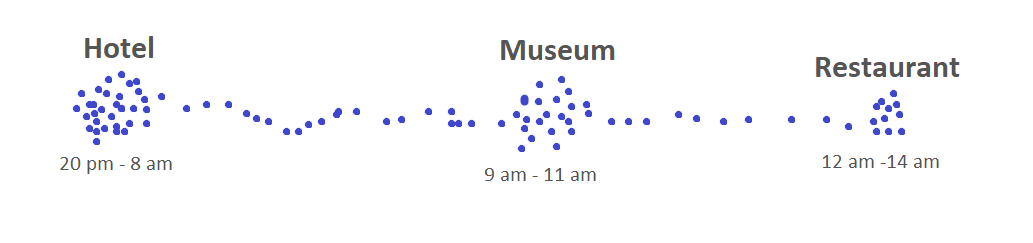
\includegraphics[width=1.0\textwidth]{Images/example_semantic-trajectory.png}
\caption{An example of a semantic trajectory}
\end{figure}
\label{fig:example_semantic_trajectory}

Similarity measures that consider both stops and moves can be important in a vast number of applications such as public transportation systems, traffic management, fraud detection, tourism, urban planning, car sharing, etc.


Only a few  similarity measures were proposed for semantic trajectories, as  \cite{Kang:2009:SMT:1529282.1529580}, \cite{Liu:2012:SMM:2442968.2442971}, \cite{Ying:2010:MUS:1867699.1867703}, and \cite{Furtado:TGIS12156}. The main problem of these measures is that they do not address all three dimensions (space, time, and semantics), as the works of \cite{Kang:2009:SMT:1529282.1529580} and \cite{Liu:2012:SMM:2442968.2442971}; or they exclusively address the stops, systematically ignoring all information about the moves, as the works of \cite{Ying:2010:MUS:1867699.1867703} and \cite{Furtado:TGIS12156}. To the best of our knowledge, none of the existing similarity measures for semantic trajectories have considered both stops and moves. The measure MSM (Multidimensional Similarity Measure) \cite{Furtado:TGIS12156}, for instance, considers only the stops, and they are treated as elements that are independent from each other, without considering the order/sequence as they appear in the trajectories. As MSM ignores the moves between stops, it can only be used to answer questions like: \emph{how similar are two trajectories $P$ and $Q$ considering their stops?}


\begin{figure}[h]
\centering
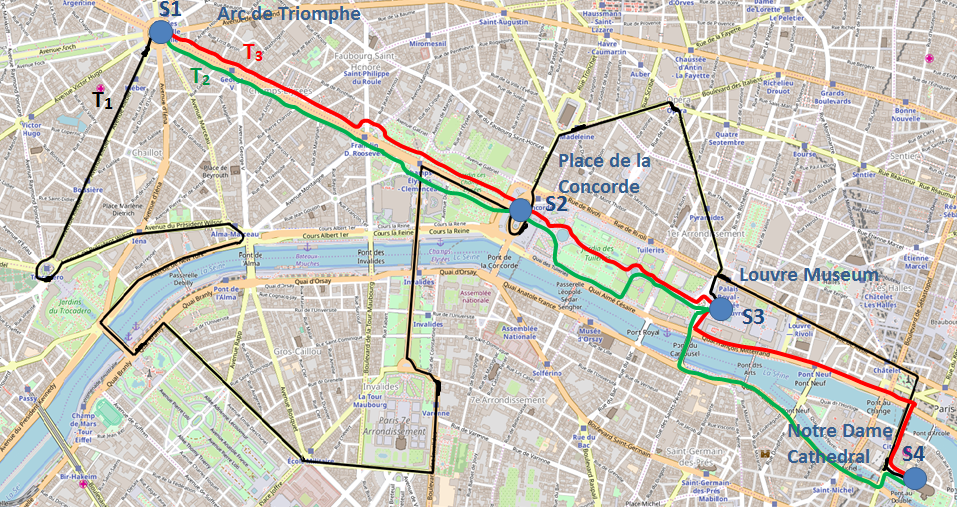
\includegraphics[width=1.0\textwidth]{Images/paris5.png}
\caption{Tourist trajectories in Paris with four stops}
\end{figure}
\label{fig:Paris}


{To better understand the need for considering both stops and moves in trajectory similarity analysis, let us consider the example in Figure \ref{fig:Paris}, for a tourism application, which shows three trajectories of tourists visiting Paris. These tourists visited four places, in this order:  Arc de Triomphe (first stop - S1), Place de la Concorde (second stop - S2), the Louvre Museum (third stop - S3), and the Notre Dame Cathedral (the last stop - S4). The three tourists visited the same places at the same order, but the tourists of trajectories $T2$ (green trajectory) and $T3$ (red trajectory) moved on foot, following the shortest path, while the tourist of trajectory $T1$ used a city tour hop on and hop off bus to appreciate the view. The question we want to answer in this thesis is \emph{how similar are trajectories $T1$, $T2$ and $T3$ considering both stops and moves?} From the figure it is clear that trajectories $T2$ and $T3$ are more similar, because they used almost the same paths between stops and moved on foot, while trajectory $T1$ has a spatially different move, performed with a different transportation mode. Now suppose that a tourism manager wants to recommend a trip to a new tourist arriving in Paris, and this new tourist wants to visit the same places visited by the tourists in the figure, but he wants to move on foot and follow the path used by the majority of the tourists.
For this case, we need to retrieve trajectories $T2$ and $T3$. 
Another example is the evaluation of the flow of tourists moving on foot between these four stops in order to eventually propose a new and direct hop on hop off tourist bus line.}

{In taxi fraud detection, for instance, a similarity measure will help to answer questions like: given two regions of interest, which is the standard path followed by the majority of the taxis and which are the outliers?
A real example of an outlier taxi trajectory is shown in Figure {\ref{fig:CRAWDAD_outlier}}, in the San Francisco dataset of the CRAWDAD project} \cite{epfl-mobility-20090224}. {In this example, given the stops Airport and  Westfield San Francisco Centre (WSFC), a similarity measure must consider both stops and moves to find the black trajectories as the most similar movements between the Airport and WSFC, and the trajectory in purple as the most dissimilar trajectory, which made a completely different and longer trip.}
 
\begin{figure}[h]
\centering
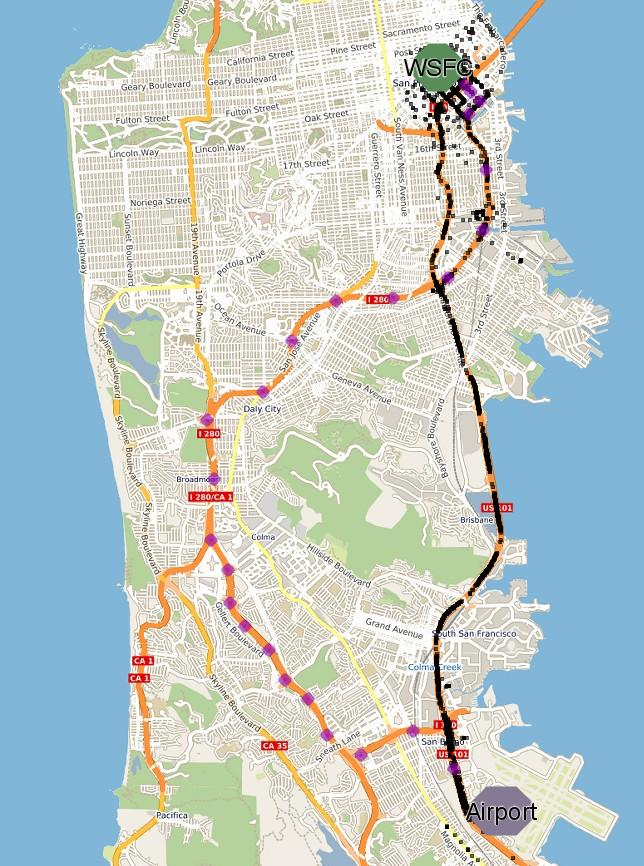
\includegraphics[width=0.5\textwidth]{Images/CRAWDAD-Outlier.jpg}
\caption{\label{fig:CRAWDAD_outlier} An outlier trajectory (in purple) going from Airport to downtown of San Francisco}
\end{figure}

In all previous examples, MSM cannot distinguish the trajectories, because it ignores the moves, and gives a similarity degree of 100\% for the trajectories in both scenarios.
Given the need of spatio-temporal similarity measures that consider both stops and moves, in this thesis we propose a new semantic trajectory similarity measure that extends MSM, proposed in \cite{Furtado:TGIS12156}, to support both stops and moves. Our approach considers the sequence of the stops, what is not supported by MSM, allows different semantics for the moves, and uses weights to provide importance degrees for stops, moves, and their attributes. 
In summary, we make the following contributions:
(i) we propose a new similarity measure for multidimensional sequences treating elements with heterogeneous dimensions, which is the case of stops and moves; (ii) the semantic similarity measure considers both \textit{stops} and \textit{moves}, as well as their space, time, and semantic dimensions, allowing the use of different distance functions for each dimension, making the measure robust for several applications; (iii) the measure is flexible enough to partially consider the order between stops and to support different weights for stops, moves, and dimensions, allowing to give more or less importance to different trajectory parts; (iv) we evaluate the proposed measure with experiments over synthetic and real data, comparing our proposal to a large number of measures developed either for raw or semantic trajectories.

\section{Objective}

The general objective of this thesis is the proposal of a novel semantic trajectory similarity measure, with proven accuracy and efficiency. We can further detail the aiming of this work in the following specific objectives:

\begin{itemize}
  \item The proposed similarity measure takes into account both \emph{stops} and \emph{moves} of the semantic trajectories;
  \item The proposed similarity measure allows the measuring of semantic trajectories considering their multiple dimensions, such as spatial, temporal, semantics, and other additional dimensions;
  \item The proposed similarity measure considers partially the sequence of the stops.
\end{itemize}

\section{Methodology}
The methodology adopted in this thesis has 8 steps:

\textit{Step} 1: Perform a review of the literature in related subjects such as trajectory similarity and semantic trajectory similarity using Google Scholar.

\textit{Step} 2: Study and implement related semantic trajectory similarity measures to find and understand limitations in related similarity measuring approaches.

\textit{Step} 3: Define a new semantic trajectory similarity measure to overcome limitations in existing similarity measures.

\textit{Step} 4: Select, organize, and pre-process datasets with real trajectory data, such as San Francisco taxi dataset from the CRAWDAD project\cite{epfl-mobility-20090224}, the Geolife dataset \cite{zheng2009mining}, and synthetic data, such as generated by Hermoupolis tool\cite{Pelekis-Hermoupolis}.

\textit{Step} 5: Evaluate the efficiency of the methods using the precision at recall \cite{BaezaYatesRibeiroNeto2011} as an information retrieval evaluation technique.

\textit{Step} 6: Comparison of the results obtained in all datasets with the most related approaches in literature.

\textit{Step} 7: Write an article describing the proposed semantic similarity measure, reporting the results of it evaluation.

\textit{Step} 8: Write the thesis describing the problem, the state-of-the-art, and the contribution for the problem solution with the advances over the state-of-the-art.

\section{Scope and Outline}

This thesis is limited to the proposal of a novel similarity measure for semantic trajectories, evaluation and comparison of this new similarity measure with the most related approaches in literature. 

The rest of this thesis is organized as follows: \textit{Chapter} \ref{sec:related} presents the basic concepts and the related works for this thesis, \textit{Chapter} \ref{sec:proposed_measure} presents the proposed similarity measure with a running example, \textit{Chapter} \ref{sec:experiments} presents experiments over real and synthetic trajectory data, \textit{Chapter} \ref{sec:discussion} presents a discussion about the choice of a measure in face of application problems, and \textit{Chapter} \ref{sec:conclusions} summarizes the contributions of this thesis, its limitations and points out future steps of the present research.


    % PARTE
    % \ifforcedinclude\else\part{Preparação da pesquisa}\fi

    % Capitulo com exemplos de comandos inseridos de arquivo externo
    %\include{chapters/chapter_1}
    
    % Capitulo de revisão de literatura
    \phantomsection


% Is it possible to keep my translation together with original text?
% https://tex.stackexchange.com/questions/5076/is-it-possible-to-keep-my-translation-together-with-original-text
\chapter[\lang{Related works}{Trabalhos relacionados}]
{
    \lang
    {Related works}
    {Trabalhos relacionados}
}
\label{sec:related}

\begin{flushright}
    \englishword{ }
\end{flushright}


% Multiple-language document - babel - selectlanguage vs begin/end{otherlanguage}
% https://tex.stackexchange.com/questions/36526/multiple-language-document-babel-selectlanguage-vs-begin-endotherlanguage

Along the last years, many similarity measures for trajectories were proposed, focusing on raw trajectories, which find the similarity between two trajectories considering spatial and temporal information. Vlachos in \cite{vlachos2002discovering} proposed LCSS, a measure in which two points \textit{match} when their distance is less than a given threshold. The longer the common subsequence of matches between two trajectories, the more similar they are. {Edit Distance with Real Penalty (ERP) is a distance function proposed for time series in }\cite{Chen:2004:MLE:1316689.1316758}. It computes the distance between two sequences of points by aligning the sequences, allowing gaps in the sequence when there are points that do not match. The gaps are penalized based on the distance of the unmatched points. Chen in \cite{Chen:2005:RFS:1066157.1066213} proposed EDR, a similarity measure for raw trajectories that calculates the edition difference between the points, as classical edit distance measures. Another measure for raw trajectories is {w-constrained discrete Frechet distance} (wDF), proposed in \cite{Ding:2008:ESJ:1440463.1440989}, considering only the spatial dimension. Although LCSS and EDR have not been proposed for this intent, both measures can be easily extended to handle other dimensions (e.g. semantics). However, that extensibility does not allow the measures to represent semantic trajectories as a sequence of heterogeneous elements, that is the case of stops and moves, because both LCSS and EDR demand that all trajectory elements should be homogeneous.

The distance measure Dynamic Time-Warping adaptive (DTWa) proposed in \cite{Shokoohi-Yekta2017} extends the classical {Dynamic Time-Warping} (DTW) \cite{berndt1994using} distance measure to multiple data dimensions. The problem of DTWa is that it deals with numeric dimensions only, and it is a distance function, not a similarity measure.

{UMS was proposed in \cite{Furtado-UMS-2018} as a new parameter-free similarity measure for raw trajectories. UMS was designed exclusively for raw trajectories, considering only the spatial dimension. The major contribution of UMS is that no distance threshold is needed, and the distance between two trajectories is computed with ellipses over every two trajectory points, so trajectories are represented as sequences of ellipses. The similarity is given by the proportion of ellipse intersection. As the ellipses are dynamically defined according to the point distance, UMS solves the problem of trajectories with distinct or varied sampling rates, by computing each ellipse size as big as necessary to cover two consecutive points. UMS outperformed all state-of-the-art works for raw trajectories developed before 2018, so it is currently the best similarity measure for raw trajectories where the spatial dimension is the most important.}

%\hl{Distinctly of the raw points measures, in the work of }\cite{Laube2005}\hl{ a raw trajectory is analyzed through the derived features of the movement, such as speed changing, momentous speed and others. The main purpose of work of Laube is to define a few behavior patterns in raw trajectories and find spatial encounters in respect to these behaviors. Using the REMO concept (RElative MOtion), it approach has as constraint that analyzed trajectories must be synchronized in time. This is not the case in real life trajectories of persons or regular vehicles, since each moving object (person, vehicles, etc) starts its movement independently each other, limiting it uses for some specific contexts, such as birds migration, wildlife monitoring, etc. In a similar way, the work proposed in } \cite{Shirabe2006}\hl{ shows that a strong correlation of motion features can help to find a linear correlation between trajectories in raw trajectory datasets. A drawback of the approach is the inability to consider the spatial and temporal location of each point. In other words, the trajectories are analyzed only by their behavior and not by their discrete points.}

The Common Visit Time Interval (CVTI) is proposed in \cite{Kang:2009:SMT:1529282.1529580} as a measure to integrate the semantic dimension of the stops with the temporal dimension. Although using different data dimensions, the measure is not extensible for other dimensions associated with the point, not allowing heterogeneous data such as stops and moves to be modeled and measured together.

In \cite{Ying:2010:MUS:1867699.1867703} the measure {Maximal Semantic Trajectory Pattern} (MSTP) is proposed, which despite being a measure for semantic trajectories, it is not able to handle multiple data dimensions. Moreover, as MSTP essentially works with the frequency at which stops are visited, it is not able to consider moves between stops.

In the work of \cite{Furtado:TGIS12156}, the MSM measure is proposed to multidimensional similarity measuring, and it is so far, the best similarity measure for semantic trajectories. In MSM all elements must be homogeneous, not allowing the representation of heterogeneous elements as stops and moves. MSM is more robust than LCSS and EDR by allowing partial dimension matching and not forcing a sequence. MSM was developed to work only with stops, and the sequence of elements is not taken into account during the similarity calculation, ignoring the order of the stops. We claim that for some applications as car sharing, new bus route planning, traffic analysis, and recommendation systems, the sequence of stops may play an important role.


    % PARTE
    % \ifforcedinclude\else\part{Referenciais teóricos}\fi

    % Capitulo de descrição da medida
    % The \phantomsection command is needed to create a link to a place in the document that is not a
% figure, equation, table, section, section, chapter, etc.
%
% When do I need to invoke \phantomsection?
% https://tex.stackexchange.com/questions/44088/when-do-i-need-to-invoke-phantomsection
\phantomsection


% Multiple-language document - babel - selectlanguage vs begin/end{otherlanguage}
% https://tex.stackexchange.com/questions/36526/multiple-language-document-babel-selectlanguage-vs-begin-endotherlanguage

\chapter[\lang{Basic concepts and the Proposed measure}{Conceitos básicos e a Medida proposta}]
{
    \lang
    {Basic concepts and the Proposed measure}
    {Conceitos básicos e a Medida proposta}
}\label{sec:proposed_measure}

    \begin{flushright}
         
    \end{flushright}

Stops and moves by definition are different and heterogeneous trajectory elements. A stop may have a spatial position, a start and end time, a category, or a set of attributes related to the category (e.g. Category hotel, stars, rate, price), etc. A move always starts and ends in a stop and may be characterized by different attributes as average speed, traveled distance, sequence of streets, duration, the sequence of raw points, etc. These attributes are defined according to the needs of the application. 

In order to deal with these heterogeneous elements (stops and moves), we introduce the concept of \emph{movement element}. A movement element is a new representation that is not treated by other measures, mainly MSM, which supports only stops. Indeed, MSM does not consider the order of trajectory elements, while in our approach we preserve the sequence of both stops and moves in a movement element.

\begin{definition}
\label{def:movement_element}
A movement element  $e=(stopS, move, stopE)$ is a tuple formed by a start stop $stopS$, the $move$ between $stopS$ and  $stopE$, and the end stop $stopE$, where stopS and stopE are two consecutive stops.
\end{definition}


Hereafter we will consider a semantic trajectory as a sequence of \textit{movement elements}, as follows: 
$ST=\langle e_1 = (s_1,m_1,s_2), e_2$\newline $= (s_2,m_2,s_3), ..., e_n = (s_n,m_n,s_{n+1}) \rangle$.

Notice that we define a movement element as a trajectory part, and this structure will be used for the proposed similarity measure, where one trajectory will be compared with another one based on their movement elements.



We analyze the similarity of a movement element $a\in A$ with another movement element $b\in B$, where A and B are semantic trajectories, in two parts: their stops and their moves. The basis for measuring the similarity of these two parts is the \emph{match} function, given in Equation \ref{func:match1}. The function returns 1 if the distance between an attribute (also called dimension) of two movement elements is less than a given threshold \emph{maxDist}, and zero otherwise. This function is used for measuring the distance of all dimensions of both: the stops and the moves.

\begin{equation}
%\scriptsize
\label{func:match1}
  match_i(a, b) = 
  \begin{cases} 
      1 & dist_i(a, b) \leq maxDist_i \\
      0 & otherwise
  \end{cases}
\end{equation}

To compute a total score for two movement elements $a$ and $b$ we define the function \emph{score(a,b)} in Equation \ref{func:score1}, where, $w_{stop}$ and $w_{move}$ are the weights of the stops and the moves, respectively, and their sum should be one. The importance of either stops or moves can vary from one application to another, so we can use the weights to give the respective importance. 


\begin{equation}
%\scriptsize
\label{func:score1}
score(a, b) = scoreStop(a, b) * w_{stop} + scoreMove(a, b) * w_{move}  
\end{equation}


In our measure we consider a score for the stops (scoreStop) and a score for the move (scoreMove). The functions \emph{scoreStop(a,b)} and \emph{scoreMove(a,b)} are defined in Equations \ref{func:scoreStop1} and \ref{func:scoreMove2}, respectively. In both equations, $r$ and $q$ are the number of dimensions (attributes) of stops and moves, respectively. The score of the stops, computed according to Equation \ref{func:scoreStop1}, is given by the average of all dimension matches of the start and end stops of two movement elements $a$ and $b$. 


\begin{equation}
%\scriptsize
\label{func:scoreStop1}
\begin{split}
  scoreStop(a, b) = \sum\limits_{i=1}^r & (match_i(a_{stopS}, b_{stopS}) + \\
  &  match_i(a_{stopE}, b_{stopE}))\div 2* w_{i}
\end{split}
\end{equation}


\begin{equation}
%\scriptsize
\label{func:scoreMove2}
\begin{split}
scoreMove(a, b)  & = 
  \begin{cases} 
      \sum\limits_{i=1}^q match_i(a_{move}, b_{move}) * w_{i} & if matchStops(a, b)\\
      0 & otherwise
  \end{cases}
\end{split}
\end{equation}


%The sum of the weights in Equations \ref{func:scoreStop1} and \ref{func:scoreMove2} should be one.
Note in Equation \ref{func:scoreMove2} that the \emph{scoreMove} depends on the function \textit{matchStops(a, b)}. {The intuition is that two moves should be evaluated only if their starting positions (starting stops) are spatially close and the ending positions (ending stops) are close as well.}
The function \emph{matchStops(a,b)} is true when the {spatial distance} between $a_{stopS}$ and $b_{stopS}$  as well as between $a_{stopE}$ and $b_{stopE}$ is less than or equal to $maxDist$.
    
    %\textcolor{red}{In real scenarios, this means that if we want to analyze movement elements, for instance, from France to Italy, we do not need to compare these trajectories with others moving from France to Spain, since the ending stop is different}.

{Figure {\ref{fig:move}} shows an example of four movement elements representing part of four trajectories. The movement elements are $e_1=<A, P_1, B>$, $e_2=<A, P_2, B>$, $e_3=<A, P_3, B>$ and $e_4=<A, P_4, C>$, where $A$, $B$, and $C$ are the stops, and $P_i$ are the moves. Considering $e_1$ and $e_4$, the function $match(P_1,P_4)$ will be executed only if the function $matchStops(B,C)$ is true, i.e., $dist(B,C) \leq  maxDist$. If $dist(B,C) > maxDist$, the value of $scoreMove(e_1,e_4)$ is zero.
%So the \emph{moves} of the movement elements $<A, P_1, B>$, $<A, P_2, B>$, $<A, P_3, B>$ will be analyzed because they have the same start and end stop.}
}

 %and three trajectories move to $B$ following three different paths.  In the example in Figure \ref{fig:move}, if we are interested in trajectories moving from A to B, our measure will only analyze the moves $P1$, $P2$, and $P3$ of trajectories going from A to B, and these three moves will not be compared with $P4$. 

%{Differences among the three movement elements rely exclusively on the differences of the move. On the other hand, the difference of these movement elements to movement element $<A, P_4, C>$ is more evident, since if it end stop is distinct, the move is distinct too. Based on this, SMSM do not compare the move of $<A, P_4, C>$ with the others movement element.}

{The function \emph{scoreMove()} guarantees a partial order in the similarity analysis. %, what has not been considered by MSM, which is the closest measure to our approach, but that considers only stops and without any order. Considering that the four movement elements in Figure {\ref{fig:move}} belong to four different trajectories, MSM would give the same similarity for the parts of the trajectories going from $A$ to $B$, because it does not look the moves, and 50\% similarity with the trajectory going from $A$ to $C$ because they share 50\% of the stops.
Suppose the example in  Figure {\ref{fig:move}} is a real scenario, where $A$, $B$, and $C$ represent  places as France, Italy, and Spain, respectively. We believe that the three trajectories going from France ($A$) to Italy ($B$) must have their move analyzed because they visit the same sequence of places, while the trajectory that goes from France ($A$) to Spain ($C$) does not share the same destination, so the move of this trajectory is not compared with the others, and the function $scoreMove()$ has values zero.}



\begin{figure}[h]
\centering
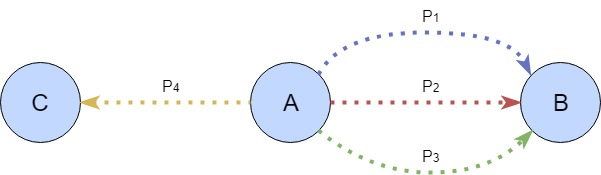
\includegraphics[width=0.75\textwidth]{Images/Toy_trajectories.jpg}
\caption{\label{fig:move} Movement elements: stop $A$ to stop $B$ with the moves $P_1$, $P_2$, and $P_3$; and Movement element: $A$ to $C$ with the move $P_4$}
\end{figure}

Having defined the score for stops and moves for comparing movement elements, Equation \ref{func:parity} defines the parity of two semantic trajectories $A$ and $B$. The parity of $A$ with $B$ is the sum of the highest score of all the elements $a \in A$ when compared with all the elements of $B$.
\begin{equation}
\label{func:parity}
parity(A, B) = \sum\limits_{a\in A} \textbf{max}\{\textit{score}(a, b) : b \in B\}
\end{equation}

Finally, we can define the global similarity of two trajectories $A$ and $B$ with $SMSM$. Equation \ref{func:SMSM1} defines the stops and moves similarity measure $SMSM(A,B)$ by the average parity of $A$ with $B$ and of $B$ with $A$. {The average parity is given by the sum of both parities over the sum of the number of elements in $A$ ($|A|$) and the number of elements in $B$ ($|B|$).}

\begin{equation}
\label{func:SMSM1}
%\scriptsize
\begin{split}
  SMSM(A, B) = 
  \begin{cases} 
      0 & if  |A| = 0 \vee |B| = 0 \\
      \frac{parity(A, B) + parity(B, A)}{|A| + |B|} & otherwise
  \end{cases}
\end{split}
\end{equation}



\section{Evaluation over a running example}

In this section we present a running example, comparing SMSM and MSM, since MSM is the closest approach.
Let us consider the two trajectories shown in Figure \ref{fig:bus}. Trajectory $Q$ represents the daily routine of a professor, that starts his day at the gym in the morning, while trajectory $P$ is the daily routine of a student, that starts his day at a coffee shop. Both trajectories visit the same places, sharing some streets, but in totally different order. The trajectories are annotated with the stop category, start and end time of the stop, an hypothetical geographic position ($x, y$) of the stop and the main street followed during the moves. So considering the {notation \textit{stop name ((x, y), [start timestamp - end timestamp])}}, the student has the following movement behavior: stays at \textit{Home} (\textit{(96,215)}, [\textit{8pm-8am}]), {then} he goes via Edu Vieira street to have breakfast at the \textit{Coffee shop} (\textit{(182,201)}, [\textit{8:50am-10am}]), and from there goes via Delfino Conti street to the \textit{University} (\textit{(59,127)}, [\textit{10:25am-6:10pm}]), finishing the day moving via Henrique Fontes street to the \textit{Gym} (\textit{(268,63)}, [\textit{7:30pm-9pm}]). The professor (trajectory $Q$) goes from \textit{Home} (\textit{(13,81)}, [\textit{7pm-7am}]) via Beira-mar avenue for jogging at the \textit{Gym} (\textit{(268,63)}, [\textit{7:30am-8:30am}]). After he goes to the \textit{Coffee shop} (\textit{(182,201)}, [\textit{8:45am-9:55am}]) via Edu Vieira street, and via Delfino Conti reaches the \textit{University} (\textit{(59,127)}, [\textit{10:15am-7:45pm}]) to teach his classes until the end of the day. We have two trajectories $P$ and $Q$ with their stops and moves annotated with the category of the place, the spatial position of the visited place, the time of the visit, and the name of the street to represent the move.
\begin{figure}[h!]
\centering
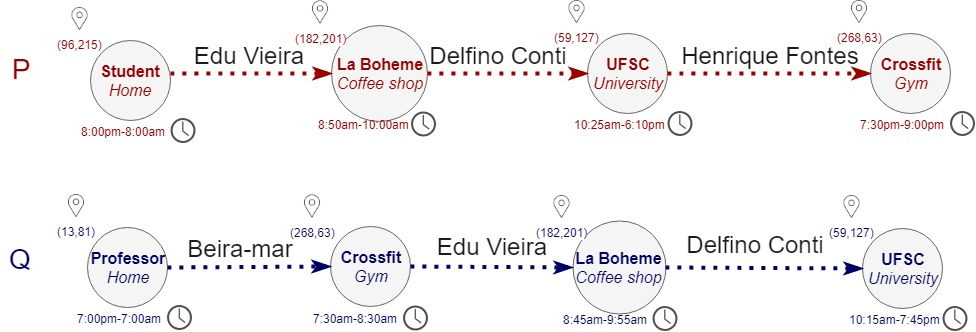
\includegraphics[width=1\textwidth]{Images/running_example.jpg}
\caption{\label{fig:bus} Semantic Trajectories $P$ (Student) and $Q$ (Professor) with stops and moves}
\end{figure}


In order to calculate the SMSM similarity value, we first need to construct all movement elements for each trajectory. Table \ref{tab:SMSM_tuples} lists these elements, where each element contains the start stop, the name of the street followed during the move, and the next stop. 

\begin{table}[h!]
\scriptsize
  \centering
 \resizebox{\linewidth}{!}{%
  \begin{tabular}{|c|c|}
  	\hline
		\textcolor{Red}{\textbf{Student (P)}} & \textcolor{Blue}{\textbf{Professor (Q)}}\\
  	\hline
      $<$Home, Edu Vieira, Coffee shop$>$&$<$Home, Beira-mar, Gym$>$\\
      $<$Coffee shop, Delfino Conti, University$>$&$<$Gym, Edu Vieira, Coffee shop$>$\\
      $<$University, Henrique Fontes, Gym$>$&$<$Coffee shop, Delfino Conti, University$>$\\
  	\hline
  \end{tabular}
  }
  \caption{Movement elements}
  \label{tab:SMSM_tuples}
\end{table}

To measure the distance between two movement elements, in this example we use the following distance functions for each stop dimension:
\begin{itemize}
  \item Space: the Euclidean distance between the centroids of the stops;
      \item  Time:  {let $[t1, t2]$ be the time interval of a stop. The time distance of two stops is given by:}
\begin{equation} \label{func:time_interval}
	dist_t(a, b) = 1 - \dfrac{duration([a.t1, a.t2] \cap [b.t1, b.t2])}{duration([min(a.t1, b.t1), max(a.t2, b.t2)])}
\end{equation}
{We use this formula in order to have a proportion of the time intersection and not an absolute value.}
  \item Semantics: the distance is equal to 0 in case of exact match and equal to 1 otherwise.
\end{itemize}

For the sake of simplicity, for the move, in this example we consider only the semantic information, i.e., the name of the followed street, where the distance is equal to 0 in case of exact match of street name and equal to 1 otherwise.
We consider that stops and moves have the same weight and also the dimensions space, time and semantics of the stops.

In this running example we use as thresholds \textit{maxDist\textsubscript{space}} = 100  and \textit{maxDist\textsubscript{time}} = 0.5, i.e. two stops are said as matched in time when both share half of their period in that stop.
With distance functions and threshold values defined and elements constructed, we use Equation \ref{func:score1} to measure the similarity values between all element dimensions, computing first the match in both start and end stops and if the stops match we compute the match for the move. 

To better understand how to measure the movement element similarity let us consider  the following two movement elements: 
\begin{itemize}

\item $element_{P}= \\ \ <Home_{[8pm-8am]}, Edu Vieira,$ $Coffee\ shop_{[8:50am-10am]}>$
\item $element_{Q}= \\ \ <Home_{[7pm-7am]}, Beira-mar, Gym_{[7:30am-8:30am]}>$ 
\end{itemize}
First, we apply the function $match()$ (Equation \ref{func:match1}) for the stops. In this case, the start stops have some degree of similarity: their semantics is the same and the time distance of $Home_{P}$ and $Home_{Q}$ is $\approx 0.15$, lower than our defined threshold of $0.5$. However, the spatial distance is $dist_{eucl}(Home_{P}, Home_{Q}) \approx 158 $, higher than the defined threshold (100), so not matching in space, only in time and semantics, leading to a similarity score of $2/3$ between start stops $Home_{[8pm-8am]}$ and $Home_{[7pm-7am]}$. The end stops (Gym and Coffee Shop) are dissimilar in space (with a distance of $\approx 163$), in time (no overlap), and in semantics, then the similarity score between both end stops is $0.0$.

 Equation \ref{func:scoreStop1} computes the stops similarity as the average similarity of start stops  and end stops as: $scoreStops($$element_{P}$, $element_{Q}$) = $(2/3 + 0) / 2 \approx 0.33$.
 As the function $matchStops()$ is false in this example since $dist_{eucl}(Coffee$ $shop_{P}, Gym_{Q}) > 100$, when applying Equation \ref{func:scoreMove2}, the function
$scoreMove()=0$. Then, Equation \ref{func:score1} computes the movement element similarity as the sum of stops similarity weighted by $w_{stops}$ and the move similarity weighted by $w_{move}$. In this example, $score($$element_{P}$, $element_{Q}$) = $(0.33 * 0.50) + (0.00 * 0.50) \approx 0.17$. Table \ref{tab:SMSM_scores} summarizes SMSM similarity scores between all movement elements.

\begin{table}[h]
\scriptsize
  \centering
 \resizebox{\linewidth}{!}{%
  \begin{tabular}{|l|c|c|c|}
  	\hline
		\backslashbox[48mm]{Q}{P}& 
        \makecell{$<$\textcolor{RawSienna}{\textbf{Home}}, Edu V., \textcolor{OliveGreen}{\textbf{Coffee}}$>$ \\ \textcolor{RawSienna}{$[$8pm-8am$]$~~\textcolor{OliveGreen}{$[$8:50am-10am$]$}} \\ \textcolor{RawSienna}{(96,215)}~~~~~~~~~~~\textcolor{OliveGreen}{(182,201)}} & 
        \makecell{$<$\textcolor{OliveGreen}{\textbf{Coffee}}, Delfino C., \textcolor{Mahogany}{\textbf{University}}$>$ \\ \textcolor{OliveGreen}{$[$8:50am-10am$]$}~~\textcolor{Mahogany}{$[$10:25am-6:10pm$]$} \\ \textcolor{OliveGreen}{(182,201)}~~~~~~~~~~~~~~~~~~~\textcolor{Mahogany}{(59,127)}} & 
        \makecell{$<$\textcolor{Mahogany}{\textbf{University}}, Henrique F., \textcolor{Fuchsia}{\textbf{Gym}}$>$ \\ \textcolor{Mahogany}{$[$10:25am-6:10pm$]$}~~\textcolor{Fuchsia}{$[$7:30pm-9pm$]$} \\ \textcolor{Mahogany}{(59,127)}~~~~~~~~~~~~~~~~~~~~\textcolor{Fuchsia}{(268,63)}}\\
  	\hline
      \makecell{$<$\textcolor{RawSienna}{\textbf{Home}}, Beira-mar, \textcolor{Fuchsia}{\textbf{Gym}}$>$\\ \textcolor{RawSienna}{$[$7pm-7am$]$}~~\textcolor{Fuchsia}{$[$7:30am-8:30am$]$} \\ \textcolor{RawSienna}{(13,81)}~~~~~~~~~~~~~~~\textcolor{Fuchsia}{(268,63)}}
      				&0.17&0&0.25\\
      \makecell{$<$\textcolor{Fuchsia}{\textbf{Gym}}, Edu V., \textcolor{OliveGreen}{\textbf{Coffee}}$>$\\ \textcolor{Fuchsia}{$[$7:30am-8:30am$]$}~~\textcolor{OliveGreen}{$[$8:45am-9:55pm$]$} \\ \textcolor{Fuchsia}{(268,63)}~~~~~~~~~~~~\textcolor{OliveGreen}{(182,201)}}
      				&0.25&0&0\\
      \makecell{$<$\textcolor{OliveGreen}{\textbf{Coffee}}, Delfino C., \textcolor{Mahogany}{\textbf{University}}$>$\\ \textcolor{OliveGreen}{$[$8:45am-9:55am$]$}~~\textcolor{Mahogany}{$[$10:15am-7:45pm$]$} \\ \textcolor{OliveGreen}{(182,201)}~~~~~~~~~~~~~~~~~~\textcolor{Mahogany}{(59,127)}}
      				&0.08&1&0\\
  	\hline
  \end{tabular}
  }
  \caption{Similarity scores for SMSM}
  \label{tab:SMSM_scores}
\end{table}

After  computing the similarity scores of both trajectories, with Equation \ref{func:parity} we compute the parity of trajectories, summing the highest scores of all movement elements of one trajectory when compared with all elements of the other trajectory. The parity calculus of $parity(P, Q) = (0.25 + 1.00 + 0.25) = 1.50$ and $parity(Q, P) = (0.25 + 0.25 + 1.00) = 1.50$.
The final SMSM score is given by Equation \ref{func:SMSM1} with $(parity(P, Q) + parity(Q, P)) / (|P| + |Q|) = (1.50 + 1.50) / (3 + 3) = 0.50$, indicating that the trajectories have some degree of similarity, since the two trajectories have several common stops at similar time, move across the same streets, but the most important is that the order of the stops is different. Notice from Table \ref{tab:SMSM_scores} that movement elements where either the start stops or the end stops match, still have a degree of similarity, which is the case of the movement elements $<Home, Edu Vieira, Coffee shop>$ and $<Home, Beira-mar, Gym>$.

{To compare SMSM with MSM, which is the closest work to our approach, we used for MSM the same thresholds for the stops and the same weights for space, time and semantics.}
%use as thresholds \textit{maxDist\textsubscript{space}} = $100$ meters and \textit{maxDist\textsubscript{time}} = $0.5$. 
MSM will measure the similarity between all stops using the same dimensions: space, time, and semantics. Let us consider the two stops at \textit{Home}. Both stops have the same semantics and their time overlap is $\approx 0.15$, lower than the defined threshold of $0.5$. As the spatial distance between both ($\approx 158$) is higher than the defined threshold ($100$), in this dimension they do not match. The similarity score between both \textit{Home} stops is the average of matched dimensions, leading to a similarity score of $2/3$, the same as SMSM. The MSM similarity scores between all stops of trajectories $P$ and $Q$ are shown in Table \ref{tab:MSM_comparision}.

\begin{table}[h]
\scriptsize
\centering
\centerline{
 \resizebox{\linewidth}{!}{%
  \begin{tabular}{|l|c|c|c|c|c|}
  	\hline
         \backslashbox[26mm]{P}{Q} & 
         \makecell{Home \\ $[$7:00pm-7:00am$]$ \\ (13,81)} & 
         \makecell{Gym \\ $[$7:30am-8:30am$]$ \\ (268,63)} & 
         \makecell{Coffee shop \\ $[$8:45am-9:55pm$]$ \\ (182,201)} & 
         \makecell{University \\ $[$10:15am-7:45pm$]$ \\ (59,127)}\\
  	\hline
        \makecell{Home \\ $[$8:00pm-8:00am$]$ \\ (96,215)} &2/3&0&1/3&1/3\\
        \makecell{Coffee shop \\ $[$8:50am-10:00pm$]$ \\ (182,201)} &0&0&1&0\\
        \makecell{University \\ $[$10:25am-6:10pm$]$ \\ (59,127)} &1/3&0&0&1\\
         \makecell{Gym \\ $[$7:30pm-9:00pm$]$ \\ (268,63)} &0&2/3&0&0\\
  	\hline
  \end{tabular}
  }
  }
  \caption{Similarity scores for MSM}
  \label{tab:MSM_comparision}
\end{table}

MSM calculates the parity between both trajectories by summing the highest scores of all stops of one trajectory compared with all stops of the other trajectory. The similarity value of MSM is given by $(parity(P, Q) + parity(Q, P)) / (|P| + |Q|) = (3.33 + 3.33) / (4 + 4) \approx 0.83 $, indicating that the two trajectories have a high similarity degree, what is not the case of the trajectories in the example. The high similarity given by MSM is due to the fact that the order of the stops is not important and the moves are not considered.

As we claimed initially, in some applications the movement sequence can be very important. In this example, SMSM evidences that, beside a strong similarity in the spatial dimension and stop categories, the sequence of stops (i.e person routine) and the moves is very dissimilar. In the following section we compare our measure with other state-of-the-art approaches, considering real trajectories.


    % PARTE
    % \ifforcedinclude\else\part{Resultados}\fi

    % Primeiro capitulo de Resultados
    % The \phantomsection command is needed to create a link to a place in the document that is not a
% figure, equation, table, section, section, chapter, etc.
%
% When do I need to invoke \phantomsection?
% https://tex.stackexchange.com/questions/44088/when-do-i-need-to-invoke-phantomsection
\phantomsection


% Multiple-language document - babel - selectlanguage vs begin/end{otherlanguage}
% https://tex.stackexchange.com/questions/36526/multiple-language-document-babel-selectlanguage-vs-begin-endotherlanguage

\chapter[Experiments]{Experimental Evaluation}\label{sec:experiments}

\begin{flushright}
     
\end{flushright}

To evaluate the proposed measure we performed three different experiments. The two first experiments use real and well known trajectory datasets: the taxi trajectories in San Francisco from the CRAWDAD project \cite{epfl-mobility-20090224} and the Geolife dataset \cite{zheng2009mining}. The third experiment uses a synthetic trajectory dataset, created using the Hermoupolis \cite{Pelekis-Hermoupolis} trajectory generator, which generates semantic trajectories with \emph{stops} and \emph{moves}. In the Geolife and taxi datasets we evaluate the similarity of both stops and moves, where the \emph{moves} similarity is evaluated considering its raw points, while in the synthetic dataset we consider several types of semantic information associated to the \emph{moves}. 

We also evaluated how SMSM is impacted by changing its parameters and compare the running time of SMSM and the other similarity measures, for both raw and semantic trajectories.

We evaluate the precision of SMSM by the retrieval-based approach (\textit{precision at recall}), computing the Area Under the Curve (AUC) and Mean Average Precision (MAP). To calculate the precision at recall, the trajectories are segregated into \textit{T\textsubscript{class}} by their classes and were used as the ground truth trajectories. For each ground truth trajectory, the $|$\textit{T\textsubscript{class}}$|$ most similar trajectories should also belong to \textit{T\textsubscript{class}}. For each one, a similarity search over the dataset is performed, ranking the trajectories until all \textit{T\textsubscript{class}} trajectories are found. Ideally, a similarity measure should return all trajectories in the ground truth between 1 to $|$\textit{T\textsubscript{class}}$|$ positions. The results of precision at each recall level are the average obtained for all \textit{T\textsubscript{class}} trajectories at that recall level. We compared SMSM with the following state-of-the-art similarity measures: MSM, LCSS, EDR, MSTP, CVTI, DTWa, wDF, and UMS.

Section \ref{sec:new_crawdad} describes the experiment with the {taxi} dataset, Section \ref{sec:geolife} details the experiments with the Geolife dataset, Section \ref{sec:hermoupolis} details the experiments with the synthetic dataset, Section {\ref{sec:sensitivity}} details the experiments changing the SMSM parameters, Section {\ref{sec:running_time}} evaluates the running time of the similarity measures, and Section {\ref{sec:discussion}} presents a discussion about the choice of a measure in face of application problems.

\section{Experiment with the taxi dataset}\label{sec:new_crawdad}

The epfl/mobility dataset contains taxi trips in San Francisco collected between May and June 2008, with an average sampling rate of about one point per minute. Each trajectory has several days of duration, what is not useful to determine similar movements around the town. For that reason, we split each taxi trajectory into short trajectories, (i) splitting when the occupation status of the taxi changed (taken or free) and (ii) splitting when a 5 minutes gap between two consecutive points was found\hl{, since if a taxi is 5 minutes not sending any GPS signal is expected the car is off and it is not moving around the city.}

\subsection{Ground truth generation}
{In this experiment we defined six distinct regions in San Francisco with high density of trajectories moving between these regions, which are shown in Figure {\ref{fig:new_sanfrancisco_map_rois}}(left). The regions are the \textbf{Park}, the \textbf{Fisherman's Wharf}, the \textbf{Pier}, the Westfield San Francisco Center (\textbf{WSFC}), the \textbf{Intersection} between highways 280 and 101, and San Francisco \textbf{Airport}. In total, there are 6940 trajectories moving between these regions.}

\begin{figure}[ht!]
\centering
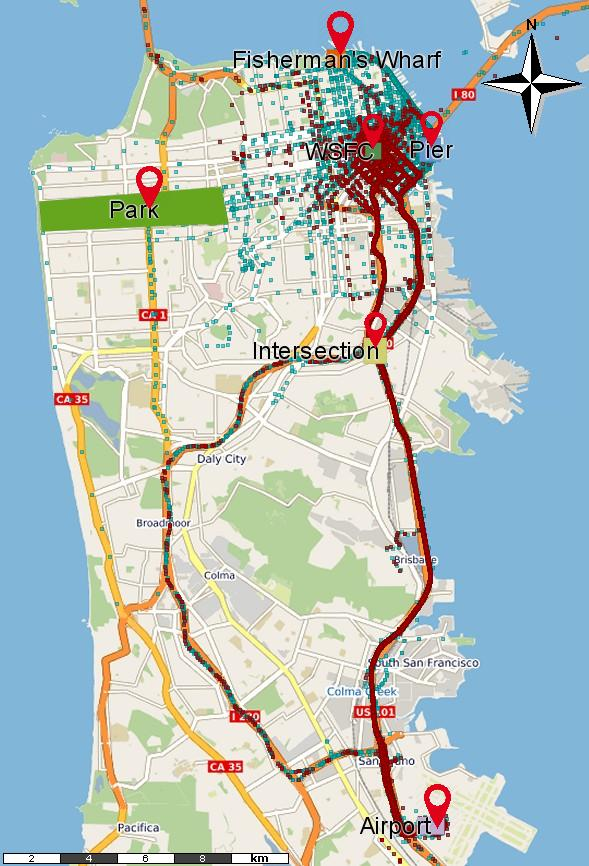
\includegraphics[width=.45\textwidth]{Images/new_CRAWDAD-Trajectories-Painted}
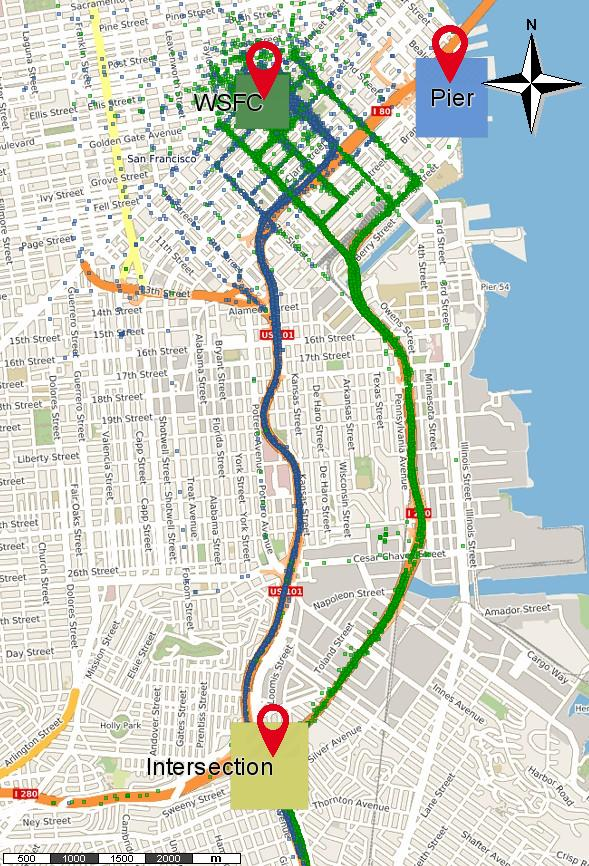
\includegraphics[width=.45\textwidth]{Images/new_CRAWDAD-Paths-Painted}
\caption{(left) All trajectories moving between the six regions, where the red points are the ground truth trajectories and the light blue points are the remaining trajectories. (right) Ground truth trajectories, where dark blue points are the trajectories moving on highway 101 and green points are trajectories using highway 280}
\label{fig:new_sanfrancisco_map_rois}
\end{figure}

As ground truth we consider the subset of trajectories moving between Airport,  Intersection, and WSFC. These trajectories were selected because they have different moves.  Figure {\ref{fig:new_sanfrancisco_map_rois}} (right) shows a zoom over the trajectories moving between  \textbf{Airport} and \textbf{WSFC}  using the \textbf{Intersection} of highways 101 (blue) and 280 (green), where we can visualize that the trajectories have different \emph{moves}. We consider as the ground truth the four distinct paths followed by the trajectories that move between these regions, which are shown in Table {\ref{tab:new_san_francisco_dataset}}. There are 145 trajectories moving from Airport in direction to WSFC via highway 101, which we define as class A1. There are 1242 trajectories moving in the opposite direction, from WSFC to the Airport by highway 101, that are labeled as class A2. There are 531 trajectories moving from Airport in direction to WSFC by highway 280, which we label as class B1, and 704 trajectories moving from WSFC in direction to Airport by highway 280, which are labeled as class B2. We assume that trajectories that belong to the same class should be more similar than trajectories of different classes.

\begin{table}[h]
\scriptsize
  \centering
  \begin{tabular}{|c|c|c|c|c|}
  \hline
 Direction & Highway & Trajectories & Class \\
  \hline
 Airport to WSFC & 101 & 145 & A1\\
 WSFC to Airport & 101 & 1242 & A2\\
 Airport to WSFC & 280 & 531 & B1\\
 WSFC to Airport & 280 & 704 & B2\\
    \hline
  \end{tabular}
  \caption{Ground truth trajectories}
  \label{tab:new_san_francisco_dataset}
\end{table}

\subsection{Results for the taxi trajectories}

In this experiment we considered the following dimensions for stops and moves: as spatial dimension of the stops we considered the centroid of the stop; as temporal dimension we used both start and end time of the stop; and as semantic information we used the name of the region (WSFC, Pier, Fisherman's Wharf, Park, Intersection, and Airport). For the moves we analyze the real movement, and use as spatial dimension the moves raw points.

For measuring the stop similarity we use: (i) the Euclidean distance for space; (ii)  distance 0 in case of exact match for semantics and 1 otherwise; and (iii) for the time dimension, where $[t1, t2]$ is the time interval of a stop, the time distance of two stops is given by  Equation {\ref{func:time_interval}}. For the moves, we consider the raw trajectory points and use the UMS measure for the move spatial similarity, because it is the most appropriate for low sampled trajectories, which is the case for this dataset.

In this experiment we consider the same weights for each dimension and for stops and moves, so 0.5 for the stops and 0.5 for the moves, and 0.33 for the dimensions space, time, and semantics. Later in the parameter analysis section we show how the results change as we vary the weights of the stops and moves, as they are the central contribution of this thesis.

As several measures were not developed for semantic trajectories, for a more fair comparison we apply existing measures over semantic trajectories and over raw trajectories. For doing so we split the experiment in two parts: 1) a \textit{precision at recall} evaluation using only semantic trajectories; and 2) a \textit{precision at recall} evaluation using the raw trajectories.

Table \ref{tab:new_san_francisco_measures} summarizes the dimensions used in each measure. To general multidimensional similarity measures as MSM, we provide as input all dimensions of each stop, namely: 1) spatial information; 2) time interval; and 3) semantic information. We extend LCSS and EDR to support multiple dimensions: given two multidimensional trajectories, two points match when all dimensions match, where each dimension has a distinct distance threshold. With those adaptations, both LCSS and EDR are used to measure similarity using the dimensions of space, time and semantics for stops. For CVTI, we provide as input the time interval of the stops and the stop names. For MSTP, we provide the stop names only.

\begin{table}[!h]
\scriptsize
  \centering
  \begin{tabular}{|l|c|c|c|c|c|}
  \hline
  & \multicolumn{4}{c|}{Semantic trajectories} & \multicolumn{1}{c|}{Raw trajectories} \\
 	\cline{2-5}
  & \multicolumn{3}{c|}{Stop} & \multicolumn{1}{c|}{Move} & \multicolumn{1}{c|}{} \\
 	\cline{2-6}
  & Space & Time & Semantics & Trajectory points & Space\\
  \hline
 SMSM & \checkmark & \checkmark & \checkmark & \checkmark & \\
 MSM & \checkmark & \checkmark & \checkmark & &\\
 MSTP &  &  & \checkmark & & \\
 CVTI & & \checkmark & \checkmark & & \\
 LCSS & \checkmark & \checkmark & \checkmark & & \checkmark \\
 EDR & \checkmark & \checkmark & \checkmark & & \checkmark \\
 DTWa &  &  &  & & \checkmark \\
 UMS & & & & & \checkmark \\
 wDF & & & & & \checkmark \\
    \hline
  \end{tabular}
  \caption{Dimensions used for each measure}
  \label{tab:new_san_francisco_measures}
\end{table}

{Table {\ref{tab:new_san_francisco_thresholds}} shows the  thresholds used for each measure. To define threshold values for the stops we experimented  a range of values on each dimension as follows: for space (distance between stop centroids) we varied the distance from 100 meters to 500 meters in a 100 meters range; and for the time distance we tested a proportion of intersection from 0\% to 100\% varying in ranges of 10 \%. For the move threshold we varied the UMS similarity for two moves from 0 to 1 in a 0.1 unit step.

Table {\ref{tab:new_sanfrancisco_measures_map_auc}} shows the comparison of SMSM with approaches developed either for raw or semantic trajectories.
For semantic trajectories, SMSM (MAP=0.84) outperformed the other measures in 50\% or more. This occurs because state-of-the-art measures do not take into account the move between two stops or consider only stops. We may notice that the second best measure for semantic trajectories is MSM, but it reaches only 39\% of precision. This shows that MSM is not robust when considering both stop and move similarity, because MSM cannot deal with moves and does not distinguish the order of the stops, i.e., the direction of the trajectories. 
For raw trajectories, SMSM (MAP=0.84) was 27 \% better than UMS (MAP=0.62) and DTWa (MAP=0.61), that were the most accurate measures apart from SMSM. Both UMS and DTWa perform worse than SMSM because on the contrary to MSM, they consider only raw trajectories, and cannot deal with stops and their semantics.}

\begin{table}[!h]
\scriptsize
  \centering
  \begin{tabular}{|c|c|c|c|c|}
  \hline
  & \multicolumn{3}{c|}{Semantic trajectories} & \multicolumn{1}{c|}{Raw trajectories} \\
 	\cline{2-5}
  & Space (meters) & Time proportion & Move & Space (meters) \\
  \hline
 SMSM & 100 & 0.3 & 0.8 & - \\
 MSM & 100 & 0.1 & - & - \\
 LCSS & 100 & 0.1 & - & 100 \\
 EDR & 100 & 0.1 & - & 100 \\
    \hline
  \end{tabular}
  \caption{Thresholds used for each measure}
  \label{tab:new_san_francisco_thresholds}
\end{table}


\begin{table}[h]
\scriptsize
  \centering
  \begin{tabular}{|l|c|c|c|c|}
  \hline
 & \multicolumn{2}{c}{Semantic} & \multicolumn{2}{|c|}{Raw} \\
 	\cline{2-5}
 & MAP & AUC & MAP & AUC \\
  \hline
SMSM & \textbf{0.84} & \textbf{0.87} & - & -\\
UMS & - & - & 0.62 & 0.66 \\
DTWa & - & - & 0.61 & 0.65 \\
wDF & - & - & 0.47 & 0.51 \\
MSM & 0.39 & 0.42 & - & - \\
EDR & 0.26 & 0.30 & 0.36 & 0.40 \\
LCSS & 0.29 & 0.33 & 0.34 & 0.38 \\
MSTP & 0.30 & 0.33 & - & - \\
CVTI & 0.28 & 0.32 & - & - \\
    \hline
  \end{tabular}
  \caption{MAP and AUC evaluation for the taxi dataset}
  \label{tab:new_sanfrancisco_measures_map_auc}
\end{table}


Figure \ref{fig:new_sanfrancisco_precision_recall} (left) and Figure \ref{fig:new_sanfrancisco_precision_recall} (right) {summarize the results of \emph{precision at recall}  of all similarity measures. On the left, SMSM was better to recover trajectories of the same class than the other methods in almost all recall levels, being around  60\% more precise than  state-of-the-art measures. On the right, we may notice that the measures developed for raw trajectories performed well, because the trajectories of the different classes are partially discriminated by the moves, characterized by the trajectory raw points. These measures do not perform better because they ignore the semantic dimensions and the stops.}


\begin{figure*}[ht!]
\centering
\centerline{
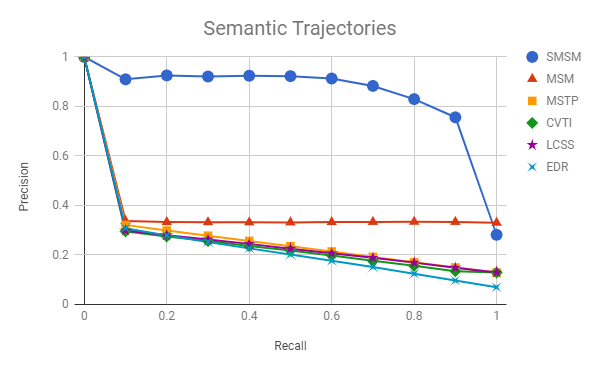
\includegraphics[width=0.5\textwidth]{Images/new_P_R-chart_San_Francisco.png}
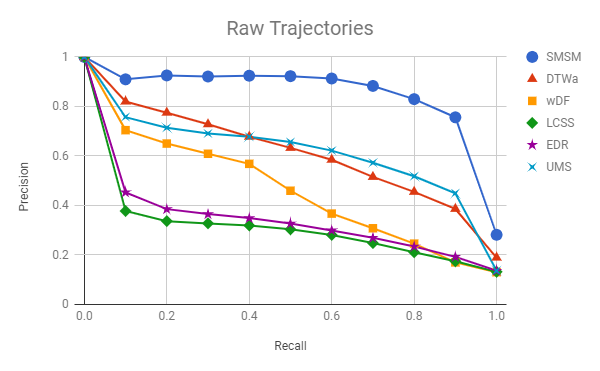
\includegraphics[width=0.5\textwidth]{Images/new_P_R-chart_San_Francisco-raw.png}
}
\caption{ Precision at recall results for semantic and raw trajectories}
\label{fig:new_sanfrancisco_precision_recall}
\end{figure*}


\section{Experiment with the Geolife Dataset}\label{sec:geolife}

The Geolife is a well-known trajectory dataset, created by Microsoft Research Asia \cite{zheng2009mining} containing trajectories of 182 users, moving around Beijing, collected between April 2007 and August 2012. As a preprocessing step, we split trajectories when a 5 minutes gap between two consecutive points was found, since the trajectories of this dataset are highly sampled (lower than 2s).

\begin{figure}[ht!]
\centering
\centerline{
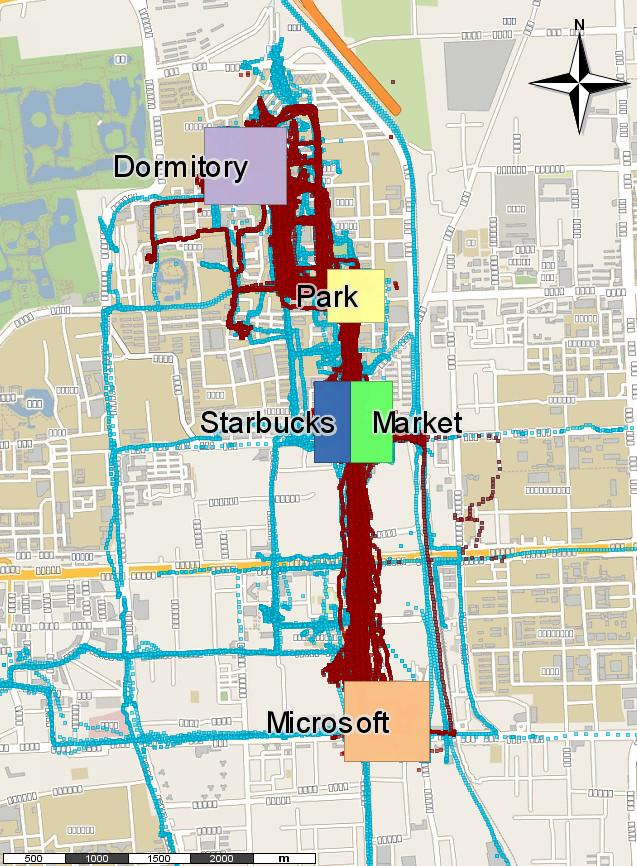
\includegraphics[width=.5\textwidth]{Images/new_Geolife-Trajectories-painted.jpg}
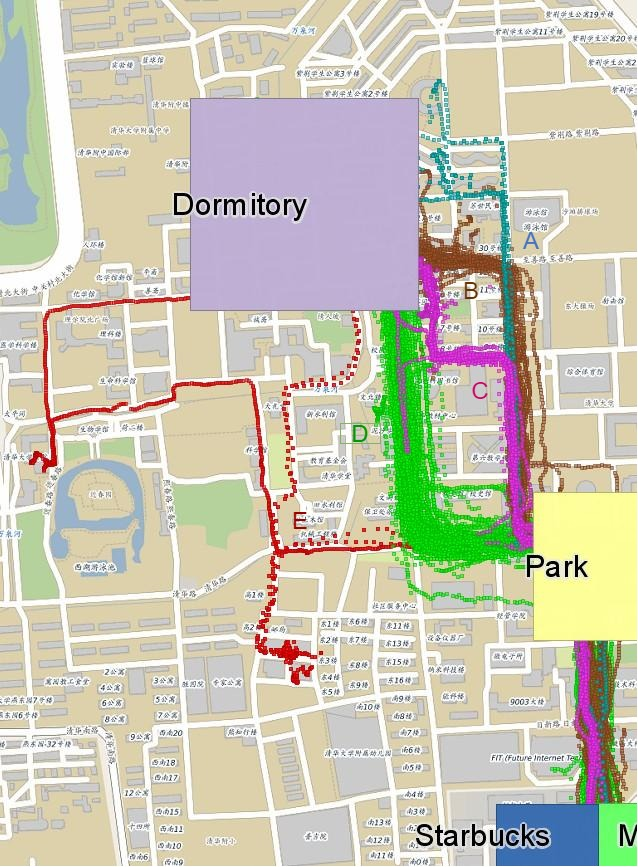
\includegraphics[width=.5\textwidth]{Images/Geolife-Paths-painted.jpg}
}
\caption{(left) All trajectories moving between the five regions, where the red points are the ground truth trajectories and the light blue points are the remaining trajectories. (right) zoom over the ground truth trajectories moving between Park and Dormitory to observe their moves}
\label{fig:geolife_map_rois}
\end{figure}


\subsection{Ground Truth Definition}
{As in the previous experiment, the Geolife dataset has no ground truth for evaluating similarity measures, so we had to generate a ground truth. We had to find stops where the objects make different moves between the stops in order to distinguish the trajectories.}
To build the ground truth, we chose an area in Beijing, where pedestrians move between the University Dormitories and Microsoft Research Office. We considered five places as stops (Microsoft, Starbucks, Market, Park and Dormitory), that are shown in Figure \ref{fig:geolife_map_rois} (left). {We selected $1976$ trajectories that pass over two or more of these places. Among the $1976$ trajectories we defined as ground truth the $337$ trajectories that go from Microsoft to Dormitory (and vice versa) passing by Park and Market or Starbucks.} We considered 5 distinct paths connecting the stops, labeled as A, B, C, D, and E, as shown in Figure \ref{fig:geolife_map_rois} (right).

In Table \ref{tab:geolife_dataset} we define as ground truth 8 distinct classes of movement based on the sequence of stops and the followed path: Microsoft to Dormitory via Market and Park by path A with 5 trajectories named as class A, Microsoft to Dormitory via Market and Park by path B with 40 trajectories named as class B, Dormitory to Microsoft via Park and Starbucks by path C with 11 trajectories named as class C, Dormitory to Microsoft via Park and Starbucks by path D with 115 trajectories named as class D1, Dormitory to Microsoft via Park and Market by path D with 7 trajectories named as class D2, Microsoft to Dormitory via Market and Park by path D with 149 trajectories named as class D3, Microsoft to Dormitory via Starbucks and Park by path D with 6 trajectories named as class D4 and Microsoft to Dormitory via Market and Park by path E with 4 trajectories named as class E.

It is worth mentioning that in this experiment, similar to the previous one, the moves are characterized by the raw trajectory points and we use these points to compare stops and moves similarity.

\begin{table}[ht!]
\scriptsize
  \centering
  \begin{tabular}{|c|c|c|c|}
  \hline
 Direction & Path &  Trajectories & Class \\
  \hline
Microsoft to Dormitory via Market and Park& A & 5 & A \\
Microsoft to Dormitory via Market and Park& B & 40&B \\
Dormitory to Microsoft via Park and Starbucks& C & 11&C \\
Dormitory to Microsoft via Park and Starbucks& D & 115&D1 \\
Dormitory to Microsoft via Park and Market& D & 7&D2 \\
Microsoft to Dormitory via Market and Park& D & 149&D3 \\
Microsoft to Dormitory via Starbucks and Park& D & 6&D4 \\
Microsoft to Dormitory via Market and Park& E & 4& E \\
    \hline
  \end{tabular}
  \caption{Classes representing distinct paths of the ground truth}
  \label{tab:geolife_dataset}
\end{table}

\subsection{Results with the Geolife dataset}

Following a similar methodology used for the previous experiment, we calculate the precision at recall for all classes in the ground truth (8), comparing the SMSM results to the other measures. The dimensions used for stops are: a) space; and b) the region name (Dormitory, Park, Starbucks, Market and Microsoft). For the moves we used the raw points of the move. The time dimension was not taken into account because in this experiment there are classes with a few trajectories and most of them do not match in time.

For measuring the stop similarity we use: (i) the Euclidean distance for space; and (ii) 1 and 0 for the semantics in case of exact match or no match, respectively. For the moves,  we consider the raw trajectory points. In this experiment we use DTW distance for analyzing the spatial similarity of the moves, because the trajectory points are highly sampled {and trajectory points are very near in space}.
For this dataset UMS is not the best measure for distinguishing the moves, since it was developed for irregular sampling. {When the points are highly sampled, UMS tends to build small ellipses, so giving low similarity degree for very similar/close trajectories}. For the weights we give the same importance for stops and moves, so we use 0.5 for stops and 0.5 for moves and for the dimensions, we use 0.5 for space and 0.5 for semantics.

Table \ref{tab:geolife_thresholds} presents the thresholds used for each measure. We defined the thresholds by running each experiment over a range of possible threshold values and the best results for each method are reported. For raw trajectories, we evaluated as threshold the  values 2, 4, 6, 8 and 10 meters because this dataset is highly sampled and is of pedestrian trajectories. The threshold for the move dimension was defined as follows: two moves are said to match if the DTW distance between them is less than the sum of the Euclidean distance of the moves. \hl{We used this approach for the move comparison because the DTW distance of two point sequences is not a bounded value as UMS, which score the similarity between 0 and 1, but an unbounded value, since DTW uses the Euclidean distance function to compare the points.}

\begin{table}[!h]
\scriptsize
  \centering
  \begin{tabular}{|c|c|c|}
  \hline
  & \multicolumn{1}{c|}{Semantic trajectories} & \multicolumn{1}{c|}{Raw trajectories} \\
 	\cline{2-3}
  & Space (meters) & Space (meters) \\
  \hline
 SMSM & 100 & - \\
 MSM & 100 & - \\
 LCSS & 100 & 8 \\
 EDR & 100 & 8 \\
    \hline
  \end{tabular}
  \caption{Thresholds used for each measure}
  \label{tab:geolife_thresholds}
\end{table}

Table \ref{tab:geolife_measures_map_auc} shows the experimental results.  {SMSM (MAP=0.94) outperforms all measures for semantic trajectories, being significantly better than MSM (MAP=0.66), which ignores the moves and the sequence of stops, so it is not able to distinguish trajectories that move in the opposite direction. On the other hand, EDR (MAP=0.72) performs better than MSM because it considers the sequence, and the order of the stops distinguishes the classes. The measures for raw trajectories perform very well because of the low number of stops in this dataset and because the raw trajectories are similar in terms of space, and the classes were build based on the moves spatial similarity, so benefiting DTWa (MAP=0.92), LCSS (MAP=0.81), and EDR (MAP=0.81). }


\begin{table}[ht!]
  \scriptsize
  \centering
  \begin{tabular}{|l|c|c|c|c|}
  \hline
 & \multicolumn{2}{c}{Semantic trajectories}& \multicolumn{2}{|c|}{Raw trajectories}\\
 	\cline{2-5}
 & MAP & AUC & MAP & AUC\\
  	\hline
SMSM & \textbf{0.94} & \textbf{0.95} & - & -\\
DTWa & - & - & 0.92 & 0.93\\
 EDR & 0.72 & 0.73 & 0.81 & 0.83\\
LCSS & 0.27 & 0.30 & 0.81 & 0.83\\
 UMS & - & - & 0.70 & 0.73\\
 MSM & 0.66 & 0.68 & - & -\\
 wDF & - & - & 0.54 & 0.58\\
CVTI & 0.30 & 0.34 & - & -\\
MSTP & 0.28 & 0.32 & - & -\\
    \hline
  \end{tabular}
  \caption{MAP and AUC evaluation with the Geolife dataset}
  \label{tab:geolife_measures_map_auc}
\end{table}


\begin{comment}
\begin{table}[ht!]
  \scriptsize
  \centering
  \begin{tabular}{|l|c|c|c|c|}
  \hline
 & \multicolumn{2}{c}{Semantic}& \multicolumn{2}{|c|}{Raw}\\
 	\cline{2-5}
 & MAP & AUC & MAP & AUC\\
  \hline
SMSM & \textbf{0.95} & \textbf{0.96} & - & -\\
DTWa & - & - & 0.93 & 0.94\\
LCSS & 0.74 & 0.75 & 0.82 & 0.84\\
 EDR & 0.74 & 0.75 & 0.81 & 0.84\\
 UMS & - & - & 0.70 & 0.73\\
 MSM & 0.69 & 0.71 & - & -\\
 wDF & - & - & 0.58 & 0.61\\
CVTI & 0.43 & 0.46 & - & -\\
MSTP & 0.41 & 0.44 & - & -\\
    \hline
  \end{tabular}
  \caption{MAP and AUC evaluation for the experiment with the Geolife dataset}
  \label{tab:old_geolife_measures_map_auc}
\end{table}
\end{comment}

{Figure {\ref{fig:geolife_precision_recall}} shows the precision at recall results. Figure {\ref{fig:geolife_precision_recall}} (left) shows that SMSM was better to recover semantic trajectories of the same class in all recall levels, while Figure {\ref{fig:geolife_precision_recall}} (right) shows that all measures developed for raw trajectories, except wDF, performed well, but  the closest results to SMSM were achieved with DTWa.}


\begin{figure*}[ht!]
\centerline{
\centering
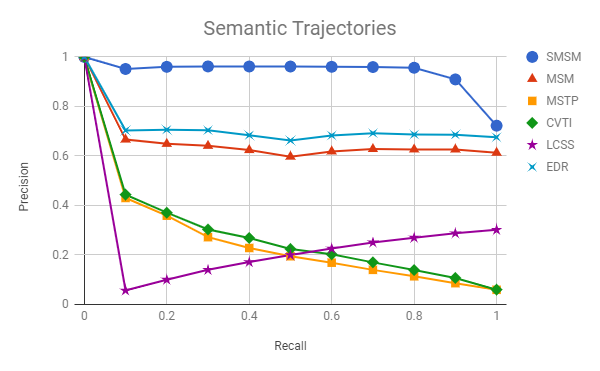
\includegraphics[width=.55\textwidth]{Images/new_P_R-chart_Geolife.png}
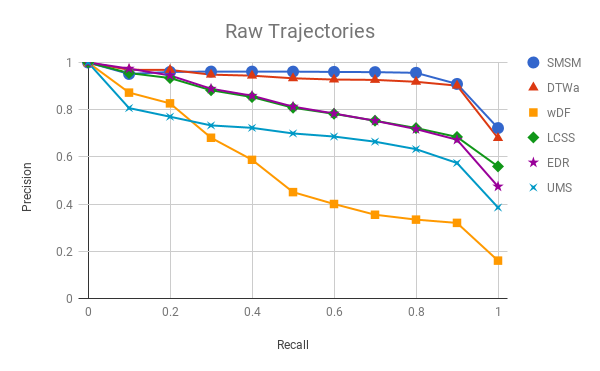
\includegraphics[width=.55\textwidth]{Images/new_P_R-chart_Geolife-raw.png}
}
\caption{Precision at recall results to semantic (left) and raw (right) trajectories}
\label{fig:geolife_precision_recall}
\end{figure*}

\section{Evaluation with a synthetic Dataset}\label{sec:hermoupolis}
The objective of this experiment with synthetic data is to evaluate trajectory similarity considering trajectories with different number of stops and the semantic dimensions of the moves, instead of the raw points of the moves that were evaluated in the previous experiments.

We generate the trajectories with the  Hermoupolis trajectory generator \cite{Pelekis-Hermoupolis}, that allows creating trajectories based on pre-defined profiles. It generates semantic trajectories where both \emph{stops} and \emph{moves} are semantically enriched with annotations defined by the user. Therefore, it is possible to enrich the \emph{moves} between the \emph{stops} with semantic information, such as the transportation mean, the goal of the \emph{move}, the name of the streets, etc. Hermoupolis has several parameters to simulate real trajectories, such as the definition of the average time of the moving object at each \emph{stop}, the standard deviation of the time of each \emph{stop}, the speed of the moves, sampling rate, and so on. We generated 440 trajectories with several stops and moves, using as semantics of the \emph{stops} the POI category and the activity performed at the \emph{stop}. For the moves we generated the raw points with the following attributes:(i) the transportation mode; (ii) the goal of the \emph{move}; (iii) the traveled distance; (iv) the average speed; and (v) the duration of the move.

There are two main differences of this experiment in relation to the previous ones: (i) the trajectories of the ground truth have a different number of stops and (ii) the moves have several and heterogeneous dimensions.

\subsection{Ground Truth Definition}
{In this experiment we defined two classes, summarized in Table {\ref{tab:hermoupolis_dataset}}: (i) students with a job (80 trajectories); and (ii) students without a job (60 trajectories). What distinguishes the classes in this experiment is not the followed paths, but mainly the time and the duration of the stops, as well as the transportation mode and the goal of the move. Besides the 140 trajectories of the ground truth, we generated 300 other trajectories in the same area, with distinct behaviors, to make the retrieval task more challenging.}

\begin{table}[ht!]
\scriptsize
  \centering
  \begin{tabular}{|c|c|c|}
  \hline
  Class & Trajectories & number of stops \\
  \hline
Student worker & 80 & 4 and 5 \\
Only student & 60 & between 4 and 7 \\
    \hline
  \end{tabular}
  \caption{Ground truth trajectories}
  \label{tab:hermoupolis_dataset}
\end{table}

{Figure {\ref{fig:hermoupolis_groundtruth}} (left) shows the generated trajectories, where the points in blue are the trajectories of the ground truth, while the brown points represent the remaining trajectories of the dataset. Some stops are Home, University, Supermarket, Restaurant, Bar, Mall, etc.
Figure {\ref{fig:hermoupolis_groundtruth}} (right) shows the trajectories of the ground truth.}

\begin{figure*}[ht!]
\centerline{
\centering
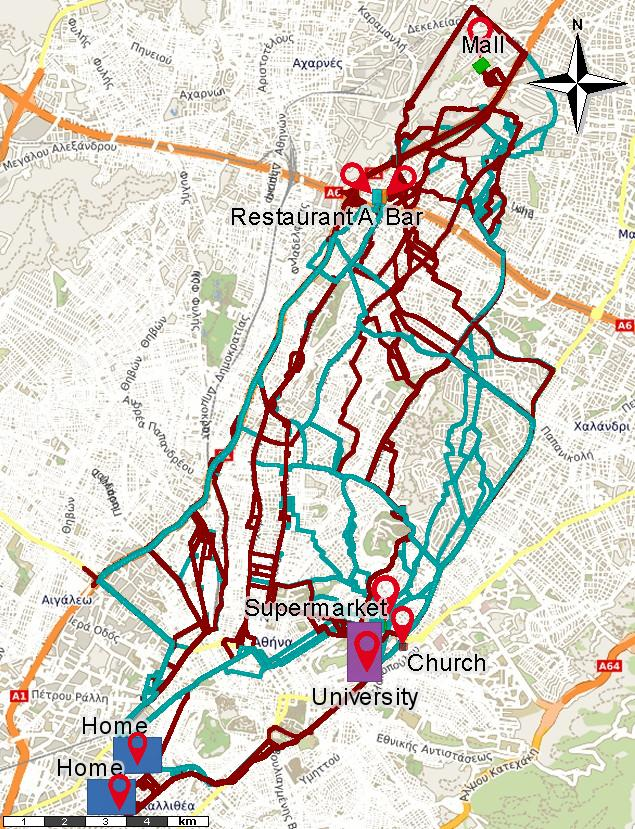
\includegraphics[width=.5\textwidth]{Images/Hermoupolis-RawPoints.jpg}
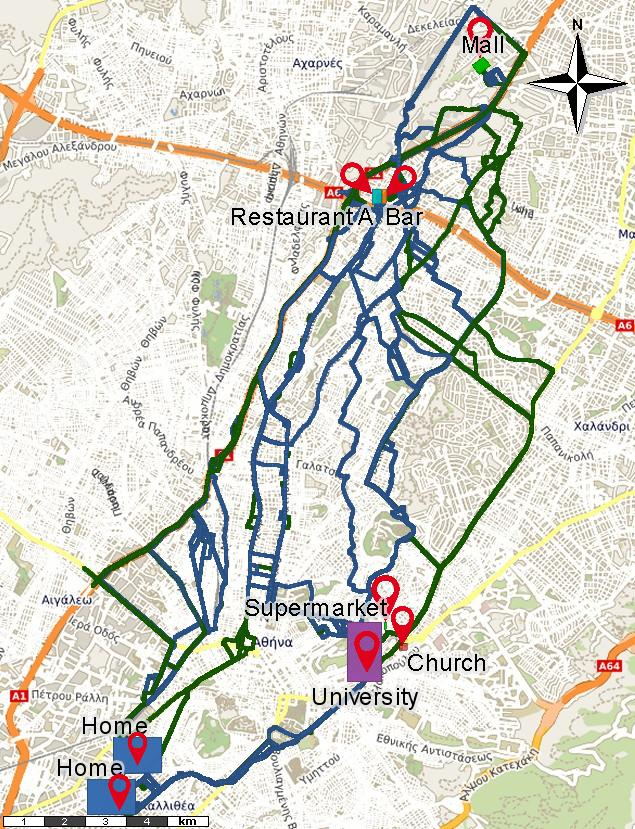
\includegraphics[width=.5\textwidth]{Images/Hermoupolis-CommercialCenter.jpg}
}
\caption{(left) Hermoupolis generated trajectories in red (ground truth) and light blue (remaining) and (right) Ground truth trajectories in green (student worker) and blue (only student).}
\label{fig:hermoupolis_groundtruth}
\end{figure*}

\subsection{Results with the Synthetic Dataset}
{Following the methodology used in the previous experiments, we calculate the precision at recall for the two classes in the ground truth, comparing the results of SMSM with the other measures. The dimensions used for the \emph{stops} are: a) the spatial centroid of the \emph{stop}; b) the duration of the \emph{stop}; and c) the \emph{stop} name (Home, Mall, University, etc). For the \emph{moves} we used several dimensions, including  the transportation mode, the goal of the move, the traveled distance, average speed, and duration.}

{For measuring the \emph{stops} similarity, we use: (i) the Euclidean distance for space; (ii) the proportion of the intersection between the time intervals of two \emph{stops}, as given by Equation {\ref{func:time_interval}}; and (iii) 1 for the semantics in case of exact match and 0 for no match. For the \emph{moves}, the transportation mode and the goal have  similarity as 1 in the case of exact match and 0 otherwise. The weights for the \emph{stops} and the \emph{moves} are the same ($0.5$), and $0.33$ for of the  dimensions space, time, and semantics. The thresholds used for each measure are shown in Table {\ref{tab:hermoupolis_thresholds}}.  As in the previous experiments, we define the thresholds for each dimension after having tested a range of values in each dimension (space and time), and the best results are reported for each measure.}

\begin{table}[!h]
\scriptsize
  \centering
  \begin{tabular}{|c|c|c|c|}
  \hline
  & \multicolumn{2}{c|}{Semantic trajectories} & \multicolumn{1}{c|}{Raw trajectories} \\
 	\cline{2-4}
  & Space (meters)& Time (intersection proportion) & Space (meters) \\
  \hline
 SMSM & 300 & 0.1 & - \\
 MSM & 300 & 0.2 & - \\
 LCSS & 100 & 0.2 & 8 \\
 EDR & 100 & 0.2 & 8 \\
    \hline
  \end{tabular}
  \caption{Spatial and temporal thresholds used for each measure}
  \label{tab:hermoupolis_thresholds}
\end{table}

Table \ref{tab:hermoupolis_measures_map_auc} presents the experimental results, in which we tested SMSM with several  attributes over the moves, and the best results where achieved with the dimensions transportation mode and goal. Comparing with measures for semantic trajectories, SMSM (MAP=0.95) was around 14\% more precise than LCSS (MAP=0.82), EDR (MAP=0.82) and MSM (MAP=0.81). The other measures for semantic trajectories had worse results, with MAP scores of 0.40 and 0.33 for MSTP and CVTI, respectively. As can be noticed in the results,  SMSM did not perform well for the dimensions duration, average speed, and traveled distance, because these dimensions are extracted from the moves raw points. As this experiment is characterized by the semantic dimensions of the moves, we can also notice that the measures for raw trajectories (EDR (MAP=0.51), DTWa (MAP=0.45), LCSS (MAP=0.44), UMS (MAP=0.29)) that performed well in the previous datasets where the moves raw points were considered, achieved at maximum 51\% of precision in the current experiment.


\begin{table}[h]
\scriptsize
  \centering
  \begin{tabular}{|l|c|c|c|c|}
  \hline
 & \multicolumn{2}{c}{Semantic} & \multicolumn{2}{|c|}{Raw} \\
 	\cline{2-5}
 & MAP & AUC & MAP & AUC \\
  \hline
SMSM (Transportation Mode)& \textbf{0.95} & \textbf{0.95} & - & -\\
SMSM (Goal)& \textbf{0.93} & \textbf{0.94} & - & -\\
SMSM (Duration)& 0.73 & 0.75 & - & -\\
SMSM (Average Speed)& 0.72 & 0.75 & - & -\\
SMSM (Traveled Distance)& 0.72 & 0.74 & - & -\\
EDR & 0.82 & 0.85 & 0.51 & 0.54 \\
LCSS & 0.82 & 0.85 & 0.44 & 0.47 \\
MSM & 0.81 & 0.83 & - & - \\
DTWa & - & - & 0.45 & 0.48 \\
MSTP & 0.40 & 0.44 & - & - \\
wDF & - & - & 0.35 & 0.39 \\
CVTI & 0.33 & 0.37 & - & - \\
UMS & - & - & 0.29 & 0.33 \\
    \hline
  \end{tabular}
  \caption{MAP and AUC evaluation for the Hermoupolis dataset}
  \label{tab:hermoupolis_measures_map_auc}
\end{table}

{Figure {\ref{fig:hermoupolis_precision_recall}} (left) shows the precision at recall curves for all similarity measures developed for semantic trajectories. SMSM, using the transportation mode as the semantic dimension of the moves, is more accurate at each level, but EDR, LCSS, and MSM had   good results despite considering only the stops. All the remaining measures present worse results. Figure {\ref{fig:hermoupolis_precision_recall}} (right) shows the precision at recall curves for similarity measures developed for raw trajectories.  In this dataset, all similarity measures developed for raw trajectories had poor results, because each class has several paths for each move, but what distinguishes the moves are not the raw points, but the transportation mode.}

\begin{figure*}[ht!]
\centerline{
\centering
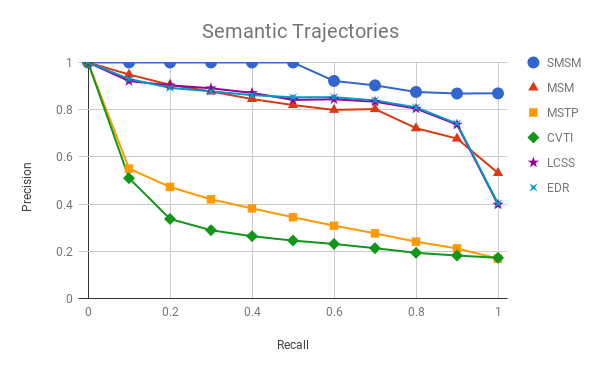
\includegraphics[width=.45\textwidth]{Images/P_R-chart_Hermoupolis_semantic.png}
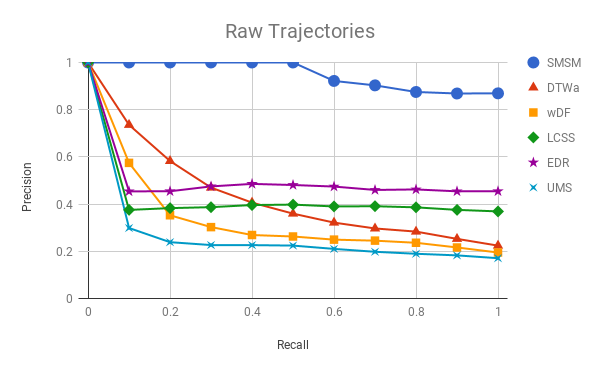
\includegraphics[width=.45\textwidth]{Images/P_R-chart_Hermoupolis_raw.png}
}
\caption{(left) Precision at recall results for semantic trajectories  and (right) Precision at recall results for raw  trajectories}
\label{fig:hermoupolis_precision_recall}
\end{figure*}


\section{Parameter Analysis}\label{sec:sensitivity}

{SMSM has two important groups of parameters: i) the \emph{weights} to define the importance of stops/moves and dimensions; and ii) the spatial \emph{threshold} to define if two stops match in order to analyze the moves.
With the weights framework, SMSM is flexible to give more or less importance to the stops, moves, and dimensions. 
}

To show the impact of the weight parameters on the similarity analysis, we evaluate the \emph{weight} of the \emph{stops} and the \emph{moves} in all experimental datasets. Table {\ref{tab:sensibility_stopmove}} shows the results for the weight varying from 0 to 1, where 0 means that the moves will be ignored and 1 means that just the moves will be considered.  As can be seen, if the influence of the \emph{moves} is ignored, i.e., weight = 0, and all importance is given to the stops, SMSM reaches a MAP score of only $0.49$ in the Taxi dataset, $0.72$ in the Geolife dataset, and $0.75$ in the synthetic dataset, indicating a confusion between the similarity of the trajectories that are also discriminated by the moves. The best average result is achieved when the weight of the \emph{moves} is set as 0.5, i.e, half of the weight goes for the stops and the other half to the moves.

\begin{table}[ht!]
  \scriptsize
  \centering
 \resizebox{\linewidth}{!}{%
  \begin{tabular}{|c|c|c|c|c|}
  \hline
Stop weight & Move weight & Taxi (MAP) & Geolife (MAP) & Hermoupolis (MAP) \\
  \hline
0.00 & 1.00 & 0.66 & 0.93 & 0.67\\
0.25 & 0.75 & 0.66 & 0.94 & 0.96\\
\textbf{0.50} & \textbf{0.50} & \textbf{0.70} & \textbf{0.94} & \textbf{0.96}\\
0.75 & 0.25 & 0.71 & 0.94 & 0.92\\
1.00 & 0.00 & 0.49 & 0.72 & 0.75 \\
    \hline
  \end{tabular}
  }
  \caption{Impact of the weights over the moves in trajectory similarity}
  \label{tab:sensibility_stopmove}
\end{table}

We also evaluate the behavior of SMSM as the spatial distance threshold of the stops varies, from very low values ($50$ meters) up to very high values ($2,000$ meters). \hl{As SMSM uses the spatial match between the start \emph{stops} and between the end \emph{stops} of two movement elements, the definition of this threshold has a great impact in the similarity score of the trajectories.} Table \ref{tab:sensibility_spatial_thresholds} shows the \hl{impact of the spatial threshold in the MAP results for the three experiments, i.e., Geolife, Taxi, and Hermoupolis datasets}. As can be observed, there is not much variation in the results for the Geolife and Taxi dataset, where the stops are \hl{spatially distant from each other}. For the synthetic dataset, when the distance threshold increases to $2,000$ meters, the precision decreases significantly, from 0.96 to 0.69, because the stops of different classes will have a spatial match \hl{and so the moves will be analyzed and many will match so confusing the classes.}

%What is important to understand from the stops spatial distance is that in the first step SMSM uses the threshold only to define if the moves will be analyzed. In a second step, even if several stops matched in space because of a large spatial threshold, they can still be distinguished by their semantics.



\begin{table}[ht!]
  \scriptsize
  \centering
  \begin{tabular}{|l|c|c|c|}
  \hline
Threshold (meters) & Geolife (MAP) & Taxi (MAP) & Hermoupolis (MAP)\\
  \hline
50 & {0.94} & 0.70 & 0.95\\
100 & {0.94} & 0.70 & 0.95\\
\textbf{300} & \textbf{0.94} & \textbf{0.70} & \textbf{0.96} \\
500 & 0.93 & 0.70 & {0.96}\\
1000 & 0.93 & 0.70 & 0.93\\
2000 & 0.92 & 0.68 & 0.69\\
    \hline
  \end{tabular}
  \caption{The MAP score for the spatial threshold variation from 50 up to 2,000 meters}
  \label{tab:sensibility_spatial_thresholds}
\end{table}


\section{Running Time Evaluation}\label{sec:running_time}

The computation time of a \hl{similarity analysis} is affected directly by two points: (i) the similarity measure employed; and (ii) the number of points of the trajectories. To evaluate the first point, in this experiment we analyze the running time of each similarity measure \hl{computing a similarity matrix between all trajectories of the datasets}, for both raw and semantic trajectories. The second point is evaluated analyzing how the number of points of the trajectories directly affects the running time in \hl{the similarity analysis} task. We use the running time of the \hl{computation of the similarity matrix}
%precision at recall experiments of Sections \ref{sec:new_crawdad}, \ref{sec:geolife}, and \ref{sec:hermoupolis} 
to evaluate the running time of the similarity measures.

Table \ref{tab:running_time_semantic} presents \hl{the average running times of 5 separate runs for each similarity measure} for semantic trajectories in seconds. The running times of SMSM were higher than all other measures. \hl{Comparing SMSM with the measures in the literature}, the running time of SMSM in the Taxi dataset (354 seconds) was about 4 times higher than the CVTI (71 seconds) running time. In the Geolife dataset, SMSM (135 seconds) was approximately 13 times higher than MSM (7.8 seconds). In the Hermoupolis dataset, the SMSM running time (4.5 seconds) is about 9 times higher than the running time of CVTI (0.5 seconds). These differences rely on how SMSM does the analysis of the \emph{move}. In the Taxi and Geolife datasets, the \emph{move} is evaluated through the raw points of the movement, and in this kind of analysis the quantity of GPS points affects proportionally the running time. In the Taxi dataset, the average of the GPS points in each \emph{move} is $\approx 8.43$, while in the Geolife dataset the average is $\approx 101.39$. On the other hand, in the Hermoupolis dataset we used the semantic information for the \emph{move} comparison (transportation mode), so for this dataset the SMSM running time was not so high. The comparison of this kind of dimension is less computationally intensive, reducing the total running time of the \hl{similarity analysis task}.%, decreasing the difference between the SMSM running time and the other similarity measures smaller. %Although the SMSM running times were higher, the SMSM MAP results were much better than the other measures.

\begin{table}[ht!]
  \scriptsize
  \centering
  \begin{tabular}{|l|c|c|c|}
  \hline
& Taxi & Geolife & Hermoupolis\\
  \hline
CVTI & \textbf{71} & 11 & \textbf{0.5}\\
EDR & 77 & 14 & 1.2\\
LCSS & 79 & 13 & 1.0 \\
MSM & 191 & \textbf{7.8} & 2.8\\
MSTP & 100 & 13 & 1.0\\
SMSM & 354 & 135 & 4.5\\
    \hline
  \end{tabular}
  \caption{The running times (in seconds) of the similarity analysis of the similarity measures for semantic trajectories}
  \label{tab:running_time_semantic}
\end{table}

Table \ref{tab:running_time_raw} shows the \hl{average running times of 2 separate runs for EDR, LCSS, UMS, and wDF similarity measures for raw trajectories. For SMSM, we use the same running times of the Table {\ref{tab:running_time_semantic}}. For DTWa, due to the very long execution time, it was performed only once.} Except for the Taxi dataset, SMSM performed much faster than other measures. That is directly related to the trajectory \hl{number of points}, since SMSM compares semantic trajectories, with less points to compare (as the \emph{stops} and the \emph{moves}), and similarity measures for raw trajectories compare each spatial point of each trajectory with the spatial points of all other trajectories. For instance, in the Taxi dataset the average \hl{number of points} of the raw trajectories $\approx 19.12$. When enriched with \emph{stops} and \emph{moves}, each trajectory has $\approx 2.72$ \emph{stops} and each move about $8.43$ points. The difference in the number of points (raw points or stops) is about 1 order of magnitude. In the Geolife dataset that difference is bigger, since the average \hl{number of points} of the raw trajectories is around to 408, while the average number of stops in the semantic trajectories $\approx 4.29$, leading to the difference being about 2 order of magnitude. The Hermoupolis dataset has the biggest difference on average \hl{number of points} of the two kinds of trajectories: the raw trajectories have on average $\approx 3,232.84$ spatial points, while the semantic trajectories have $\approx 5.23$ \emph{stops} in each trajectory on average, almost 3 orders of magnitude of difference.

\begin{table}[ht!]
  \scriptsize
  \centering
  \begin{tabular}{|l|c|c|c|}
  \hline
& Taxi & Geolife & Hermoupolis\\
  \hline
DTWa	& 780	        & 28,527        & 91,286\\
EDR		& 259	        & 6,404	        & 20,027\\
LCSS	& 258	        & 6,190	        & 20,580\\
UMS		& 681	        & 5,760	        & 17,410\\
wDF		& \textbf{225}	& 1,291	        & 3,004\\
SMSM    & 354           & \textbf{135} & \textbf{4.5}\\
    \hline
  \end{tabular}
  \caption{The running time (in seconds) of the precision at recall evaluation for raw trajectories}
  \label{tab:running_time_raw}
\end{table}

\hl{Although it is slower in the similarity analysis task, SMSM is much more precise in the information retrieval task than the literature similarity measures for semantic trajectories, as presented in Sections {\ref{sec:new_crawdad}}, {\ref{sec:geolife}}, and {\ref{sec:hermoupolis}}. Apart from SMSM, the most precise similarity measures were the measures for raw trajectories. However, as can be seen in Table {\ref{tab:running_time_raw}}, all these measures are highly impacted by trajectories with large number of points.}
Figure \ref{fig:running_time_graphs} shows how the distinct representation of a trajectory (either between raw or semantic trajectory) can impact in the running times in the \hl{similarity analysis task}. Figure \ref{fig:running_time_crawdad} shows the running times only in the Taxi dataset. As we previously stated, in this dataset the difference between the average \hl{number of points} in the raw trajectories and the \hl{number of \emph{stops} in the} semantic trajectories is about 1 order of magnitude. \hl{In this dataset, three} similarity measures for raw trajectories (wDF, LCSS, and EDR) were faster than SMSM. But as we stated in the Taxi dataset experiment in Section \ref{sec:new_crawdad}, SMSM outperformed all similarity measures for both raw and semantic trajectories in the precision at recall task.
Figures \ref{fig:running_time_geolife} and \ref{fig:running_time_hermoupolis} show the running times in the Geolife and Hermoupolis datasets, respectively. In these two datasets, since the difference between the \hl{number of points} in the raw \hl{trajectories and the number of \emph{stops}} in the semantic trajectories is greater than 2 orders of magnitude, the running times of the similarity measures for raw trajectories are much higher than the running time of SMSM. \hl{The SMSM retrieval information results in both datasets were greater than the results for all similarity measures for raw trajectories.}

\begin{figure*}[ht!]
    \centering
    \begin{subfigure}{0.45\textwidth}
        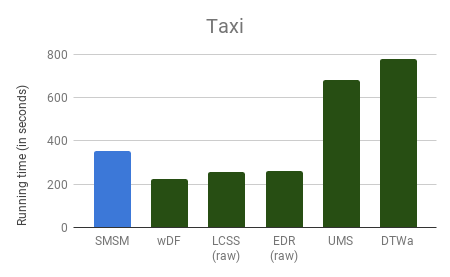
\includegraphics[width=\linewidth]{Images/running_time_CRAWDAD.png}
        \caption{}
        \label{fig:running_time_crawdad}
    \end{subfigure}
    \begin{subfigure}{0.45\textwidth}
        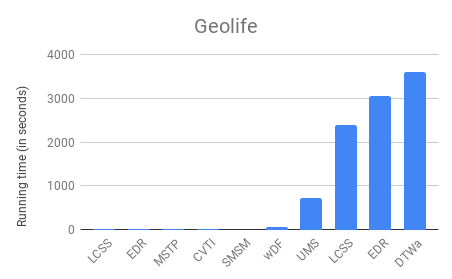
\includegraphics[width=\linewidth]{Images/running_time_Geolife.png}
        \caption{}
        \label{fig:running_time_geolife}
    \end{subfigure}\hfill % <-- added
    \begin{subfigure}[c]{0.5\textwidth}
        \centering
        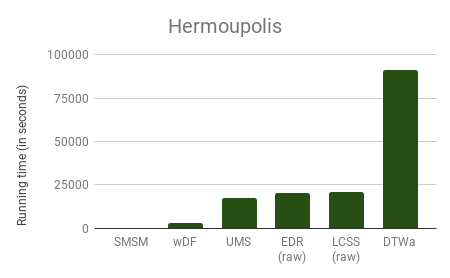
\includegraphics[width=\linewidth]{Images/running_time_Hermoupolis.png}
        \caption{}
        \label{fig:running_time_hermoupolis}
    \end{subfigure}\hfill % <-- added
    \caption{The running time of each measure in the following datasets: (a) Taxi, (b) Geolife, and (c) Hermoupolis. The running times of the similarity measures for raw trajectories are in green and the running time of SMSM is in blue.}
    \label{fig:running_time_graphs}
\end{figure*}

The higher precision in the retrieval information tasks in all experiments and the shortest running times \hl{in the similarity analysis task} show SMSM as a more powerful similarity measure when the movement of the moving object is relevant.

\section{Discussion}\label{sec:discussion}

{Trajectory data can have several formats. Depending on the format and the application requirements, different trajectory analysis and mining methods will be needed, and so different similarity measures can be applied. For applications that use raw GPS data, as trajectories of taxis, buses, or cars, with the intend to detect, for instance, traffic conditions or traffic jams, the most appropriate measures are UMS and DTWa. UMS is robust for trajectories with different sampling rates or different distances between trajectory points (the case when a trajectory varies the speed in a city), because instead of using a radius around each trajectory point to find the similar trajectories in the spatial neighbourhood, it uses ellipses between every two trajectory points, and the size of the ellipses is dinamically defined based on the distance between two trajectory points. UMS is not the best measure in highly sampled trajectories, where the ellipses are very small, and in this case DTWa is  a good choice.}

{For applications that use GPS trajectories annotated only with stops or where the moves are not important, or trajectories extracted from social media data, which are more sparse and that do not have moves, the best measure is MSM. MSM is useful in applications where one is interested in finding users that visit the same places, at similar times, but where the order of the visits is not important. In tourism applications where the analyst wants to find similar tourist trajectories to either predict or to recommend the next place to be visited, MSM is not appropriate because it ignores the order. When the sequence of the visited places is important, even when the details about the moves are not, SMSM is more appropriate, because it considers the order of the stops.}

{For dealing with GPS trajectories enriched with both stops and moves, and the spatial, temporal or semantic characteristcs of both stops and moves are important, SMSM is the most appropriate measure. In a tourism application, for instance, where the tourist has a time constraint to visit a city, a sequence of visits can be recommended based on the similarity analysis of other tourists that visited the same city. SMSM is also robust in applications that focus on the most similar paths or popular routes between stops.}

{It is important to emphasize that in applications where the spatial movement of the moves is important, i.e., the raw trajectory points, SMSM can use UMS for the move similarity when trajectories have low sampling rate and DTW when trajectories have high sampling rate.}


    % Segundo capitulo de Resultados
    % The \phantomsection command is needed to create a link to a place in the document that is not a
% figure, equation, table, section, subsection, chapter, etc.
%
% When do I need to invoke \phantomsection?
% https://tex.stackexchange.com/questions/44088/when-do-i-need-to-invoke-phantomsection
\phantomsection


% Multiple-language document - babel - selectlanguage vs begin/end{otherlanguage}
% https://tex.stackexchange.com/questions/36526/multiple-language-document-babel-selectlanguage-vs-begin-endotherlanguage

\chapter[Discussion]{Discussion: Applications versus Measures}\label{sec:discussion}


\begin{flushright}
 
\end{flushright}


{Trajectory data can have several formats. Depending on the format and the application requirements, different trajectory analysis and mining methods will be needed, and so different similarity measures can be applied. For applications that use raw GPS data, as trajectories of taxis, buses, or cars, with the intend to detect, for instance, traffic conditions or traffic jams, the most appropriate measures are UMS and DTWa. UMS is robust for trajectories with different sampling rates or different distances between trajectory points (the case when a trajectory varies the speed in a city), because instead of using a radius around each trajectory point to find the similar trajectories in the spatial neighbourhood, it uses ellipses between every two trajectory points, and the size of the ellipses is dinamically defined based on the distance between two trajectory points. UMS is not the best measure in highly sampled trajectories, where the ellipses are very small, and in this case DTWa is  a good choice.}

{For applications that use GPS trajectories annotated only with stops or where the moves are not important, or trajectories extracted from social media data, which are more sparse and that do not have moves, the best measure is MSM. MSM is useful in applications where one is interested in finding users that visit the same places, at similar times, but where the order of the visits is not important. In tourism applications where the analyst wants to find similar tourist trajectories to either predict or to recommend the next place to be visited, MSM is not appropriate because it ignores the order. When the sequence of the visited places is important, even when the details about the moves are not, SMSM is more appropriate, because it considers the order of the stops.}

{For dealing with GPS trajectories enriched with both stops and moves, and the spatial, temporal or semantic characteristcs of both stops and moves are important, SMSM is the most appropriate measure. In a tourism application, for instance, where the tourist has a time constraint to visit a city, a sequence of visits can be recommended based on the similarity analysis of other tourists that visited the same city. SMSM is also robust in applications that focus on the most similar paths or popular routes between stops.}

{It is important to emphasize that in applications where the spatial movement of the moves is important, i.e., the raw trajectory points, SMSM can use UMS for the move similarity when trajectories have low sampling rate and DTW when trajectories have high sampling rate.}




    % Finaliza a parte no bookmark do PDF
    % para que se inicie o bookmark na raiz
    % e adiciona espaço de parte no Sumário
    \phantompart

    % Conclusão (outro exemplo de capítulo sem numeração e presente no sumário)
    % The \phantomsection command is needed to create a link to a place in the document that is not a
% figure, equation, table, section, subsection, chapter, etc.
%
% When do I need to invoke \phantomsection?
% https://tex.stackexchange.com/questions/44088/when-do-i-need-to-invoke-phantomsection
\phantomsection

% ---
% Considerações Finais (outro exemplo de capítulo sem numeração e presente no sumário)
% ---

\chapter[Conclusion]{\lang{Final Remarks}{Considerações Finais}} \label{sec:conclusions}
\phantomsection
\addcontentsline{toc}{chapter}{Final Remarks}%
In this work we proposed SMSM, a new similarity measure for semantic trajectories that supports both stops and moves.  To the best of our knowledge, SMSM is the first semantic trajectory similarity measure that deals with both stops and moves and their space, time and semantic dimensions. The proposed similarity measure is robust  to consider multiple dimensions of stops and moves, where a move, for instance, can be represented as raw points, the traveled distance, the major direction, the names of streets, the transportation mode, etc.

SMSM supports the definition of weights for stops, moves and dimensions, so the measure is flexible to give more or less importance for specific parts of trajectories. On the other hand, these weights may be difficult to estimate from the user point of view, but in case he has no knowledge about the domain, the best is to define the same weight for all elements.

We performed experiments using real \hl{and synthetic} data of distinct contexts, including car trajectories and pedestrian trajectories. By evaluating SMSM with an information retrieval approach, we show that SMSM was more accurate than other measures developed either for raw or semantic trajectories.

SMSM requires a full spatial match between the start and end stop of two movement elements to evaluate the move. In future works we will study an extension of SMSM to evaluate the move in cases where the final stops of two movement elements do not have a match.




    % ELEMENTOS PÓS-TEXTUAIS
    \postextual
    \setlength\beforechapskip{0pt}
    \setlength\midchapskip{15pt}
    \setlength\afterchapskip{15pt}

    % Referências bibliográficas
    \begingroup
        % Using BibTeX to make a list of references without having citations in the body of the document?
        % https://tex.stackexchange.com/questions/17128/using-bibtex-to-make-a-list-of-references-without
        % \nocite{*}

        % How to modify line spacing per entry of bibliography?
        % https://tex.stackexchange.com/questions/163559/how-to-modify-line-spacing-per-entry-of-bibliography
        \linespread{1.18}\selectfont
        \printbibliography
    \endgroup

    % Glossário, consulte o manual da classe abntex2 para orientações sobre o glossário.
    % \ifforcedinclude\else\glossary\fi

    % Apêndices, inicia os apêndices
    \begin{apendicesenv}
        % Imprime uma página indicando o início dos apêndices
        %\ifforcedinclude\else\partapendices\fi

        \setlength\beforechapskip{50pt}
        \setlength\midchapskip{20pt}
        \setlength\afterchapskip{20pt}

        %%
% How to fix the Underfull \vbox badness has occurred while \output is active on my memoir chapter style?
% https://tex.stackexchange.com/questions/387881/how-to-fix-the-underfull-vbox-badness-has-occurred-while-output-is-active-on-m
%

% ---

\lang
{\chapter[Appendix A]{Since this page is not being completely filled, it is generating the bottom bottom of the page}}
{\chapter[Apêndice A]{Como esta página não está sendo completamente preenchida, ele está gerando a caixa inferior inferior da página}}
% ---


% Multiple-language document - babel - selectlanguage vs begin/end{otherlanguage}
% https://tex.stackexchange.com/questions/36526/multiple-language-document-babel-selectlanguage-vs-begin-endotherlanguage
\begin{otherlanguage*}{english}

 

1. How to display the font size in use in the final output,
2. How to display the font size in use in the final output,
3. How to display the font size in use in the final output,
4. How to display the font size in use in the final output,
5. How to display the font size in use in the final output,
6. How to display the font size in use in the final output,
7. How to display the font size in use in the final output,
8. How to display the font size in use in the final output,
9. How to display the font size in use in the final output,


% As this page is not being completely filled, it is generating the page bottom bad box.
% Fix Underfull \vbox (badness 10000) has occurred while \output is active
%
% \flushbottom vs \raggedbottom
% https://tex.stackexchange.com/questions/65355/flushbottom-vs-raggedbottom
\newpage



\section[Some encoding tests]{ }

1. How to display the font size in use in the final output,
2. How to display the font size in use in the final output,
3. How to display the font size in use in the final output,
4. How to display the font size in use in the final output,
5. How to display the font size in use in the final output,
6. How to display the font size in use in the final output,

7. How to display the font size in use in the final output,
8. How to display the font size in use in the final output,
9. How to display the font size in use in the final output,
10. How to display the font size in use in the final output,
11. How to display the font size in use in the final output,
12. How to display the font size in use in the final output,

\subsection{ }

1. How to display the font size in use in the final output,
2. How to display the font size in use in the final output,
3. How to display the font size in use in the final output,
4. How to display the font size in use in the final output,
5. How to display the font size in use in the final output,
6. How to display the font size in use in the final output,

7. How to display the font size in use in the final output,
8. How to display the font size in use in the final output,
9. How to display the font size in use in the final output,
10. How to display the font size in use in the final output,
11. How to display the font size in use in the final output,
12. How to display the font size in use in the final output,

\subsubsection{ }

1. How to display the font size in use in the final output,
2. How to display the font size in use in the final output,
3. How to display the font size in use in the final output,
4. How to display the font size in use in the final output,
5. How to display the font size in use in the final output,
6. How to display the font size in use in the final output,

7. How to display the font size in use in the final output,
8. How to display the font size in use in the final output,
9. How to display the font size in use in the final output,
10. How to display the font size in use in the final output,
11. How to display the font size in use in the final output,
12. How to display the font size in use in the final output,

\subsubsubsection{ }

1. How to display the font size in use in the final output,
2. How to display the font size in use in the final output,
3. How to display the font size in use in the final output,
4. How to display the font size in use in the final output,
5. How to display the font size in use in the final output,
6. How to display the font size in use in the final output,
7. How to display the font size in use in the final output,

8. How to display the font size in use in the final output,
9. How to display the font size in use in the final output,
10. How to display the font size in use in the final output,
11. How to display the font size in use in the final output,
12. How to display the font size in use in the final output,


Lipsum me [31-35]

\end{otherlanguage*}



    \end{apendicesenv}

    % Anexos, inicia os anexos
    \begin{anexosenv}
        % Imprime uma página indicando o início dos anexos
        %\ifforcedinclude\else\partanexos\fi

        \setlength\beforechapskip{50pt}
        \setlength\midchapskip{20pt}
        \setlength\afterchapskip{20pt}

        %%
% How to fix the Underfull \vbox badness has occurred while \output is active on my memoir chapter style?
% https://tex.stackexchange.com/questions/387881/how-to-fix-the-underfull-vbox-badness-has-occurred-while-output-is-active-on-m
%

% ----------------------------------------------------------
\chapter{\lang{Article published in SOBRAEP magazine}{Artigo publicado}}
% ----------------------------------------------------------


% Multiple-language document - babel - selectlanguage vs begin/end{otherlanguage}
% https://tex.stackexchange.com/questions/36526/multiple-language-document-babel-selectlanguage-vs-begin-endotherlanguage
\begin{otherlanguage*}{english}

% An environment for setting \emergencystretch locally
% https://tex.stackexchange.com/questions/84510/an-environment-for-setting-emergencystretch-locally
{
    \setlength{\emergencystretch}{10pt}
    \section[English guidelines for publication]
    {English guidelines for publication - TITLE HERE (14 PT TYPE SIZE, UPPERCASE, BOLD, CENTERED)}
}
    \noindent\textbf{Abstract:}
    The objective of this document is to instruct the authors about the preparation of the
    manuscript for its submission to the Revista Eletrônica de Potência (Brazilian Power Electronics
    Journal).~The authors should use these guidelines for preparing both the initial and final
    versions of their paper. Additional information about procedures and guidelines for publication
    can be obtained directly with the editor, or through the web site
    \url{http://www.sobraep.org.br/revista}. This text was written according to these guidelines

\end{otherlanguage*}

% What is a “Overfull \hbox (9.89561pt too wide)”?
% https://tex.stackexchange.com/questions/111948/what-is-a-overfull-hbox-9-89561pt-too-wide
interwordspace: \the\fontdimen2\font

interwordstretch: \the\fontdimen3\font

emergencystretch: \the\emergencystretch\par\relax


\modifiedincludepdf{-}{ArtigoSOBRAEP}{pictures/SOBRAEP.pdf}{0.9}



        %%
% How to fix the Underfull \vbox badness has occurred while \output is active on my memoir chapter style?
% https://tex.stackexchange.com/questions/387881/how-to-fix-the-underfull-vbox-badness-has-occurred-while-output-is-active-on-m
%

% ----------------------------------------------------------
\lang
{\chapter[Sample example]{How to display the font size in use in the final output}}
{\chapter[Anexo exemplo]{Como exibir o tamanho da fonte em uso na saída final}}
% ----------------------------------------------------------


% Multiple-language document - babel - selectlanguage vs begin/end{otherlanguage}
% https://tex.stackexchange.com/questions/36526/multiple-language-document-babel-selectlanguage-vs-begin-endotherlanguage
\begin{otherlanguage*}{english}

 

1. How to display the font size in use in the final output,
2. How to display the font size in use in the final output,
3. How to display the font size in use in the final output,


\section[Some encoding tests]{ }

1. How to display the font size in use in the final output,
2. How to display the font size in use in the final output,
3. How to display the font size in use in the final output,
4. How to display the font size in use in the final output,
5. How to display the font size in use in the final output,
6. How to display the font size in use in the final output,

7. How to display the font size in use in the final output,
8. How to display the font size in use in the final output,
9. How to display the font size in use in the final output,
10. How to display the font size in use in the final output,
11. How to display the font size in use in the final output,
12. How to display the font size in use in the final output,

\subsection{ }

1. How to display the font size in use in the final output,
2. How to display the font size in use in the final output,
3. How to display the font size in use in the final output,
4. How to display the font size in use in the final output,
5. How to display the font size in use in the final output,
6. How to display the font size in use in the final output,

7. How to display the font size in use in the final output,
8. How to display the font size in use in the final output,
9. How to display the font size in use in the final output,
10. How to display the font size in use in the final output,
11. How to display the font size in use in the final output,
12. How to display the font size in use in the final output,

\subsubsection{ }

1. How to display the font size in use in the final output,
2. How to display the font size in use in the final output,
3. How to display the font size in use in the final output,
4. How to display the font size in use in the final output,
5. How to display the font size in use in the final output,
6. How to display the font size in use in the final output,

7. How to display the font size in use in the final output,
8. How to display the font size in use in the final output,
9. How to display the font size in use in the final output,
10. How to display the font size in use in the final output,
11. How to display the font size in use in the final output,
12. How to display the font size in use in the final output,

\subsubsubsection{ }

1. How to display the font size in use in the final output,
2. How to display the font size in use in the final output,
3. How to display the font size in use in the final output,
4. How to display the font size in use in the final output,
5. How to display the font size in use in the final output,
6. How to display the font size in use in the final output,
7. How to display the font size in use in the final output,

8. How to display the font size in use in the final output,
9. How to display the font size in use in the final output,
10. How to display the font size in use in the final output,
11. How to display the font size in use in the final output,
12. How to display the font size in use in the final output,


Lipsum me [55-65]

\end{otherlanguage*}



    \end{anexosenv}

    % INDICE REMISSIVO
    \ifforcedinclude\else
        \phantompart
        \printindex
    \fi

\end{document}

